%This Source Code Form is subject to the terms of the Mozilla Public License, v. 2.0. If a copy of the MPL was not distributed with this file, You can obtain one at http://mozilla.org/MPL/2.0/.
%%%
% LaTeX Template for Thesis submitted to AG-Bloemer
% This is just a guideline - modify as you like :)
% Last Update: 13-01-2017
% In case of questions/problems/proposals you can write, call or visit me
% http://cs.uni-paderborn.de/cuk/personal/sascha-brauer/
%%%

\documentclass{cukthesis} % add [german] if required

%This Source Code Form is subject to the terms of the Mozilla Public License, v. 2.0. If a copy of the MPL was not distributed with this file, You can obtain one at http://mozilla.org/MPL/2.0/.

\def\Title{Classical Simulation of Quantum Circuits with Restricted Boltzmann Machines} % Hier Titel eintragen / Enter your title here
\def\Author{Jannes Stubbemann} % Hier Namen eintrage / Enter your name here
\def\Degree{Master} % Master
\def\SecondExaminer{Dr. Robert Schade} % Zweitgutachter / Second Examiner
%This Source Code Form is subject to the terms of the Mozilla Public License, v. 2.0. If a copy of the MPL was not distributed with this file, You can obtain one at http://mozilla.org/MPL/2.0/.

% Graphical Libs
\usepackage{graphicx}
\usepackage{setspace}

% Add additional packages as required
%This Source Code Form is subject to the terms of the Mozilla Public License, v. 2.0. If a copy of the MPL was not distributed with this file, You can obtain one at http://mozilla.org/MPL/2.0/.

% Math Defs
\renewcommand{\epsilon}{\varepsilon}
\DeclareMathOperator*{\argmax}{arg\,max}
\DeclareMathOperator*{\argmin}{arg\,min}

\newcommand*{\bfrac}[2]{\genfrac{\lbrace}{\rbrace}{0pt}{}{#1}{#2}} %Fraction withour bar

% Misc
\newcommand{\clearemptydoublepage}{\newpage{\pagestyle{empty}\cleardoublepage}}

\newcommand\qthead[2]{\makebox[42pt][c]{\textbf{#1}}\makebox[260pt][c]{\textbf{#2}}\smallskip\hrule\medskip}
\newcommand\qtline[2]{\makebox[42pt][c]{#1}\makebox[260pt][c]{\begin{quantikz}& #2 & \qw \end{quantikz}}}
\newenvironment{qtab}{\par\bigskip\bgroup\parindent32pt\obeylines}{\egroup\bigskip}

% Add additional style definitions as required
\tikzset{arrowed/.style={decorate,
decoration={show path construction, 
moveto code={},
lineto code={
\draw[#1] (\tikzinputsegmentfirst) --  (\tikzinputsegmentlast);
},
curveto code={},
closepath code={},
}},arrowed/.default={-stealth}}

\pgfplotsset{gradient function/.initial=f,
dx/.initial=0.01,dy/.initial=0.01}
\pgfmathdeclarefunction{xgrad}{2}{%
\begingroup%
\pgfkeys{/pgf/fpu,/pgf/fpu/output format=fixed}%
\edef\myfun{\pgfkeysvalueof{/pgfplots/gradient function}}%
\pgfmathparse{(\myfun(#1+\pgfkeysvalueof{/pgfplots/dx},#2)%
-\myfun(#1,#2))/\pgfkeysvalueof{/pgfplots/dx}}%
 % \pgfmathsetmacro{\mysum}{\mysum+\myfun(\value{isum},#2)}%
\pgfmathsmuggle\pgfmathresult\endgroup%
}%
\pgfmathdeclarefunction{ygrad}{2}{%
\begingroup%
\pgfkeys{/pgf/fpu,/pgf/fpu/output format=fixed}%
\edef\myfun{\pgfkeysvalueof{/pgfplots/gradient function}}%
\pgfmathparse{(\myfun(#1,#2+\pgfkeysvalueof{/pgfplots/dy})%
-\myfun(#1,#2))/\pgfkeysvalueof{/pgfplots/dy}}%
 % \pgfmathsetmacro{\mysum}{\mysum+\myfun(\value{isum},#2)}%
\pgfmathsmuggle\pgfmathresult\endgroup%
}%

\pgfplotsset{compat=1.16}

\makeglossaries
\newacronym{nisq}{NISQ}{Noisy Intermediate-Scale Quantum}
\newacronym{rbm}{RBM}{Restricted Boltzmann Machine}
\newacronym{rcs}{RCS}{Random Circuit Sampling}
\newacronym{qaoa}{QAOA}{Quantum Approximate Optimization Algorithm}
\newacronym{tvd}{TVD}{Total Variation Distance}
\newacronym{ucsb}{UCSB}{The University of Santa Barbara, California}
\newacronym{bqp}{\textbf{BQP}}{Bounded-Error Quantum Polynomial-Time}
\newacronym{bpp}{\textbf{BPP}}{Probabilistic Polynomial-Time}
\newacronym{iqp}{IQP}{Instantaneous Quantum Polynomial-Time}
\newacronym{sr}{SR}{Stochastic Reconfiguration}
\newacronym{mcmc}{MCM}{Monte Carlo Markov Chain}

\begin{document}

\bibliographystyle{plain}

\pagenumbering{roman}
   
%This Source Code Form is subject to the terms of the Mozilla Public License, v. 2.0. If a copy of the MPL was not distributed with this file, You can obtain one at http://mozilla.org/MPL/2.0/.

\thispagestyle{empty}
\begin{titlepage}
\begin{center}

	\begin{minipage}{14cm}		
		\hspace*{1.9cm}
		
\includegraphics[height=4cm]{figures/upb_logo_en}\\
		\hspace*{1.15cm}
		\begin{minipage}{14.5cm}
			\vspace*{5pt}
			\textsf{\noindent
			Faculty of Computer Science, Electrical Engineering and Mathematics\\
			Department for Quantum Computation
			}
		\end{minipage}		
	\end{minipage}\\[60pt]
	
	\begin{doublespace}
		{\Huge\textbf{\Title}}\\[30pt]
	\end{doublespace} 
	
	{\Large 
		\ifgerman
			\Degree arbeit
		\else
			\Degree 's Thesis
		\fi
	}\\[6pt]
		\ifgerman
			im Rahmen des Studiengangs Informatik\\
			zur Erlangung des Grades
		\else
			in Partial Fulfillment of the Requirements for the\\
			Degree of
		\fi
		\\[6pt]
  	{\Large \Degree\ of Science}\\[54pt] % Replace if different
	
	\ifgerman
		von\\
	\else
		by\\
	\fi
	{\scshape\large \Author}\\[54pt]
	
	\ifgerman
		vorgelegt bei:\\
	\else
		submitted to:\\
	\fi
	
	{\large Jun. Prof. Dr. Sevag Gharibian \\
	\ifgerman
		und
	\else
		and
	\fi
	\\[6pt]
	\large \SecondExaminer}\\[30pt]

	{Paderborn, \today}
	
\end{center}
\end{titlepage}
\clearpage

%This Source Code Form is subject to the terms of the Mozilla Public License, v. 2.0. If a copy of the MPL was not distributed with this file, You can obtain one at http://mozilla.org/MPL/2.0/.
	
	\ifgerman\else
	\chapter*{Declaration}\vspace{-24pt}
	
	(Translation from German)\bigskip
	
	\noindent I hereby declare that I prepared this thesis entirely on my own and have not used outside sources
	without declaration in the text. Any concepts or quotations applicable to these sources are
	clearly attributed to them. This thesis has not been submitted in the same or substantially similar
	version, not even in part, to any other authority for grading and has not been published elsewhere.

	\section*{Original Declaration Text in German:}

	\fi
	\ifgerman
	\chapter*{Erklärung}
	\else
	\section*{Erklärung}
	\fi
	
	Ich versichere, dass ich die Arbeit ohne fremde Hilfe und ohne Benutzung anderer als der
	angegebenen Quellen angefertigt habe und dass die Arbeit in gleicher oder ähnlicher Form
	noch keiner anderen Prüfungsbehörde vorgelegen hat und von dieser als Teil einer
	Prüfungsleistung angenommen worden ist. Alle Ausführungen, die wörtlich oder sinngemäß~
	übernommen worden sind, sind als solche ge\-kenn\-zeich\-net.
	
	\vspace{40pt}
	
	\begin{center}
		\begin{tabular}{l p{0.1\textwidth} r}
		  \cline{1-1} \cline{3-3}
		  \begin{minipage}[t]{0.4\textwidth}
		    \centering
			\ifgerman
			Ort, Datum
			\else
			City, Date
			\fi
			\end{minipage}
			&
			\begin{minipage}[t]{0.2\textwidth}
			\end{minipage}
			&
			\begin{minipage}[t]{0.4\textwidth}
			  \centering
			\ifgerman
			Signatur
			\else
			Signature
			\fi
			\end{minipage}
		\end{tabular}
	\end{center}

\chapter*{Acknowledgements}

I would first like to express my gratitude to my supervisor 
Jun. Prof. Dr. Sevag Gharibian who guided me through this 
thesis. His door was always open for discussions on the topic. 
He allowed this thesis to be my own work, and steered me into the right direction
whenever needed. He introduced me to experts in the field and made it possible 
for me to discuss my ideas with them.

Secondly, I want to thank Prof. Dr. Eyke H{\"u}llermeier, who 
helped me figuring out how to generate a balanced set of training samples.

Further, I want to thank Norbert Schuch, who helped me to understand the neat 
mathematical tricks in the original papers about NQS. I am grateful for Ronald de Wolf who 
took the time to discuss the underlying ideas with Sevag and me. 
Johannes Pausch proposed ideas to resolve some of the initial obstacles
in making the simulations work. Robert Schade was of big help in setting 
up the experiments on the Noctua Cluster.

Additionally, I want to thank Lisa Clau{\ss}en, Nahuel Miranda, Dorian Rudolph, Harry Duwe,
and Lisanne Visser for proof-reading. Last but not least, I want to thank my family 
and Lisanne for providing emotional support throughout the course of this thesis.

\chapter*{\centering \begin{normalsize}Abstract\end{normalsize}}
 
Random circuit sampling provides a benchmarking tool for noisy intermediate-scale quantum (NISQ)
devices and simulations.
This thesis is the first to study the abilities of restricted Boltzmann machines (RBMs)
to sample from the output distribution of such random quantum circuits. 
Variations of Stochastic Reconfiguration and AdaMax are compared for a range of training samples 
and iterations. Total variation distance (TVD) and cross entropy difference are measured 
and compared as performance metrics.
The results show that RBMs are able to simulate random quantum circuits with 4 qubits 
and a depth of up to 20 cycles accurately. When trained with AdaMax, the best 
performing RBMs were able to approximate the average true output distribution with a TVD of 0.00 
on all circuit depths.
The non-diagonal single-qubit gates can be applied within less than 100 training iterations. 
The accuracy of the RBMs had been higher the more training samples were available.
The software developed in the progress of this thesis is publicly available on GitHub. 
It can be adapted to simulate random circuits with a wider range of qubits. It 
further provides a simple interface to run quantum circuits given in the QASM format. This thesis
can act as a reference for suitable training parameters of the RBMs, which have not been 
included in related works.

\tableofcontents 

\printglossaries 
% If you have figures, uncomment this 
\listoffigures 

% If you have algorithms, uncomment this
\listofalgorithms
  
\cleardoublepage
\pagenumbering{arabic}

% Input your files here!

\chapter{Introduction}

\paragraph{The Relevance of Quantum Computing.}
Computers can be programmed to solve a wide range of problems.
While they can solve some problems efficiently, 
other problems require exponential time or memory. The simulation 
of quantum physical systems is such a problem that requires 
exponential resources \cite{nielsen2002quantum}.  
These simulations could help in the design 
of new materials and in drug discovery \cite{8585034}.

The computational complexity of simulating quantum systems led 
Richard Feynman to propose the concept of a quantum computer in 1982 \cite{feynman1982simulating}. 
Quantum computers work fundamentally different from classical computers by 
harnessing quantum physics for computation. Large-scale quantum computers have the potential
to simulate the physics of quantum systems efficiently \cite{Zalka_1998}.
Since Feynman's proposal in 1982, researchers are making progress in building small-scale 
quantum devices and understanding their computational capabilities and limitations.

Among the discoveries of the potential of the computation power of quantum computers is Shor's algorithm \cite{shor1997factorisation}: 
In 1994, Peter Shor discovered a quantum algorithm that is able to solve the 
factorization problem in polynomial time. This makes quantum computers a potential threat to 
today's internet security protocols. Most of these protocols are based on the assumption 
that the factorization problem cannot be solved efficiently, and that it would take thousands of years to find the 
prime factors of the public encryption keys.

\paragraph{Near-Term Quantum Computing and Quantum Supremacy.}
Even though error-corrected large-scale quantum computers are probably still 
years away, so-called noisy-intermediate scale 
quantum (NISQ) devices represent the first generation of quantum devices.
Studying their capabilities and limits could enable us to harness possible advantages 
of quantum computers already today. Moreover, it might be of further help understanding
the limits of large scale quantum computers \cite{Preskill_2018}.

In 2019, researchers from Google and the University of Santa Barbara (\gls{ucsb}), California, built a 
53 qubit quantum processor, called Sycamore. They performed a calculation on it that they claimed could not be 
performed on a classical computer \cite{martines2019supremacy}. This moment was highly anticipated 
as "quantum supremacy", a term coined by John Preskill in 2012 \cite{preskill2012quantum}. In the experiments, 
samples from random quantum circuits were drawn with the Sycamore processor.
The random circuit sampling experiment was specifically tailored 
to the demonstration of quantum supremacy \cite{Boixo2018supremacy}.

\paragraph{Machine Learning for the Classical Simulation of Quantum Computing.}
To understand the capabilities of such NISQ devices, one also has to understand 
the limits of classical computation. Following the recent success of machine learning in 
many scientific and industrial domains, in 2017, Carleo and Troyer applied restricted Boltzmann machines (RBMs),
one class of recurrent neural networks,
to simulate wave functions of different many-body quantum systems classically \cite{carleo2017solving}.
Their results showed that RBMs are able to offer a compact representation of wave functions 
of different many-body quantum systems. In 2018, 
J\'{o}nsson et al. adapted the framework to simulate small quantum programs with 
RBMs \cite{jnsson2018neuralnetwork}. Recently, Medvidovic and Carleo used the 
same approach for a noisy simulation of the 
\gls{qaoa} with up to 53 qubits \cite{medvidovic2020classical}.

\paragraph{Scope of the Thesis.}
This thesis investigates the abilities of RBMs to simulate the random circuit sampling 
experiments conducted in Google's supremacy experiments on the Sycamore processor \cite{martines2019supremacy}. 
The objective of this thesis is to examine if RBMs are able to sample from the output distribution 
of small random circuit instances.

Stochastic Reconfiguration (SR) \cite{sorella1998green} and 
AdaMax \cite{kingma2014adam} are compared as two different optimization algorithms for the 
adaption of the RBM's parameters. Both methods have successfully been used before to train RBMs 
for the representation of quantum system states \cite{jnsson2018neuralnetwork,carleo2017solving,carleo2018constructing,medvidovic2020classical}.
A direct comparison of both methods has not been done so far. 

Additionally, a range of training samples and training iterations 
is tested to gain insights into the training process and the required computational resources. 
These parameters have not been reported in related works. One goal of this thesis is 
to act as a reference for suitable training parameters. 

\gls{tvd}) and the cross entropy difference are used as 
performance metrics. This allows for an empirical comparison of \gls{tvd} and cross entropy difference 
on small random circuits.

Understanding the
fidelities with which RBMs can simulate quantum circuits could help to understand
the limits of classical computation. The software developed as part of this thesis 
might further help to study algorithms designed for NISQ devices. To support 
further research, it is published as 
an open source library on GitHub \cite{NQS2020}.
The experiments are conducted on the Noctua cluster located at the 
University of Paderborn, Germany \cite{noctua2020}.

\paragraph{Structure of the Thesis.}
This thesis consists of three parts: 
In the first part (Chapter~\ref{sec:notation} to ~\ref{sec:rbm}), the mathematical 
notation is introduced and the theoretical framework is explained. In the 
following part (Chapter~\ref{sec:experiments}), 
the experimental setup is described and the results are presented. 
In the last part (Chapter~\ref{sec:discussion}), the results are summarized and discussed.
Furthermore, ideas for future research are given.

Chapter~\ref{sec:notation} introduces the mathematical notation used throughout this 
thesis.

In chapter~\ref{sec:quantum_computing}, the foundations of quantum computing are introduced. 
Starting with a single qubit in section~\ref{sec:qubits}, the mathematical framework of multi-qubit systems is derived
in section~\ref{sec:multiplequbitsandentanglement}. The notation and applications 
of quantum gates are explained in section~\ref{sec:quantum_gates} before small quantum circuits are shown
in section~\ref{sec:quantum_circuits}. The chapter closes with an overview of quantum complexity 
theory in section~\ref{sec:quantum_computational_complexity}.

Chapter~\ref{sec:rcs} explains the concepts of random circuit sampling as a quantum supremacy experiment.
First, the definition of quantum supremacy and different proposals for possible experiments 
are given in section~\ref{sec:quantum_supremacy}. 
In section~\ref{sec:cross_entropy} and~\ref{sec:supremacy_regime} the 
cross entropy difference, which is the main metric of random circuit sampling, is derived.
The structure of the considered random circuits is explained in section~\ref{sec:random_circuit_design}.
In the last part of the chapter (section~\ref{sec:experiments_sycamore}), the supremacy experiment conducted by Google and the \gls{ucsb} 
and its results are discussed.

In chapter~\ref{sec:rbm}, the concept of the Boltzmann machine is introduced. 
Starting with general Boltzmann machines in section~\ref{sec:gbm}, restricted 
Boltzmann machines are explained in section~\ref{sec:rbms}.
Sections~\ref{sec:gibbsSampling} and ~\ref{sec:learning} explain how 
Boltzmann machines can be trained to resemble the probability distribution implied by a given set of samples.
The chapter closes with section~\ref{sec:applicationToQuantumComputing} which explains
how restricted Boltzmann machines can be applied to the simulation of quantum circuits.

The experiments and obtained results are described in chapter~\ref{sec:experiments}. 
The experimental setup is detailed in section~\ref{sec:setup}. The results 
for the different training strategies are presented in section~\ref{sec:results}.

The thesis closes with a discussion of the results in chapter~\ref{sec:discussion}.
Highlights and limitations of the experiments are described. 
Directions for future research are proposed as well.



\chapter{Nomenclature and Notation}
\label{sec:notation}

This chapter introduces mathematical notations and expressions used throughout 
this study. Its focus is on linear algebra, the mathematical foundation of 
\textit{quantum mechanics}. It is thought as a lookup reference for the following chapters.

Vectors are represented in the \textit{Bra-ket} notation. \textit{Ket}-vectors $\Ket{\psi}$ denote 
column vectors:

\begin{equation}
   \Ket{\psi} = \begin{pmatrix} \alpha \\ \beta \end{pmatrix}.
\end{equation}

The \textit{bra} $\Bra{\psi}$ of a vector $\Ket{\psi}$ is its hermitian conjugate, 
$\Bra{\psi} = \Ket{\psi}^{\dagger}$. It is the transpose of the vector with complex-conjugated 
entries. For the ket-vector $\Ket{\psi}$ above, the corresponding bra-vector would be:

\begin{equation}
   \Bra{\psi} = \begin{pmatrix}
      \alpha^* & \beta^*
   \end{pmatrix},
\end{equation}

where the complex-conjugate of some complex number $\alpha = a + b i$ is 
defined as $\alpha^* = a - b i$. Using this notation, the \textit{inner product} of two vectors
$\Ket{\psi}$ and $\Ket{\phi}$ can be written as:

\begin{equation}
   \Braket{\psi | \phi} = \sum_j \psi_j^* \phi_j.
\end{equation}

The \textit{outer product} $\Ket{\psi} \Bra{\phi}$ defines the matrix $A$ with entries 
$a_{ij}$ given by:

\begin{equation}
   a_{ij} = \psi_i \phi^*_j.
\end{equation}

The class of matrices of special interest in quantum computing are \textit{unitary} matrices.
A complex-valued square matrix $U$ is unitary if:

\begin{equation}
   U U^{\dagger} = U^{\dagger}U = I.
\end{equation}

Unitary matrices are norm preserving and thus represent rotations in the vector space.
The \textit{tensor product} $\cdot \otimes \cdot$ of two matrices $A=\begin{pmatrix}
   a_{11} & a_{12} \\ a_{21} & a_{22}
\end{pmatrix}$ and $B= \begin{pmatrix}
   b_{11} & b_{12} \\ b_{21} & b_22
\end{pmatrix}$ is defined as:

\begin{align}
   A \otimes B &= \begin{pmatrix}
      a_{11} B & a_{12} B \\ a_{21} B & a_{22} B
   \end{pmatrix} \\
   &= \begin{pmatrix}
      a_{11} b_{11} & a_{11} b_{12} & a_{12} b_{11} & a_{12} b_{12} \\
      a_{11} b_{21} & a_{11} b_{22} & a_{12} b_{21} & a_{12} b_{22} \\ 
      a_{21} b_{11} & a_{21} b_{12} & a_{22} b_{11} & a_{22} b_{12} \\
      a_{21} b_{21} & a_{21} b_{22} & a_{22} b_{21} & a_{22} b_{22}
   \end{pmatrix}.
\end{align}

The dimensions of the tensor product of two matrices with dimensions $n_A \times m_A$ and $n_B \times m_B$ 
is $n_An_B \times m_Am_B$. The tensor product for vectors is defined accordingly.
The \textit{Kroenecker Delta} $\delta_{ij}$ sometimes occurs in quantum physics. It is defined as:

\begin{equation}
   \delta_{ij} =
    \begin{cases}
            1, &         \text{if } i=j,\\
            0, &         \text{if } i\neq j.
    \end{cases}.
\end{equation}

\chapter{Quantum Computing}

This chapter gives an introduction to the field of \textit{Quantum Computation}. It covers the basics of qubits, quantum gates and circuits, and gives an overview of quantum complexity classes. The chapter is based on \cite{nielsen2002quantum}, which offers a profound introduction into the field.

\section{Qubits}

While classical computers harness classical physical phenomena like electrical current to perform calculations, quantum computers harness 
\textit{quantum mechanical} effects. The simplest quantum mechanical system is a quantum bit, or
\textit{qubit} for short. It is the fundamental building block of a quantum computer.

Mathematically, a qubit is a two-dimensional complex-valued unit vector,
also called the \textit{state vector} or \textit{wave function}:

\begin{equation}
  \label{eq:qubit1}
  \Ket{\psi} = \begin{pmatrix} \alpha \\ \beta \end{pmatrix}
\end{equation}

with \textit{amplitudes} $\alpha, \beta \in \mathbb{C}$ and $|\alpha|^2 + |\beta| ^2 = 1$ . 
Rewriting $\Ket{\psi}$ as

\begin{equation}
  \Ket{\psi} = e^{i \gamma} \left( \cos{\frac{\theta}{2}} \Ket{0} + e^{i \rho} \sin{\frac{\theta}{2}} \Ket{1} \right)
\end{equation}

with $\theta, \rho, \gamma \in \mathbb{R}$
allows an intuitive interpration of a qubit as a point on the surface of the three-dimensional unit sphere,
called the \textit{Bloch Sphere}, which is visualized in figure
\ref{fig:blochsphere}. The factor $e^{i \gamma}$ in front is called a
\textit{global phase} and can be ignored:

\begin{equation}
  \Ket{\psi} = \cos{\frac{\theta}{2}} \Ket{0} + e^{i \rho} \sin{\frac{\theta}{2}} \Ket{1}.
\end{equation}

\begin{figure}[H]
  \label{fig:blochsphere}
  \centering
  \begin{tikzpicture}

    % Define radius
    \def\r{3}

    % Bloch vector
    \draw (0,0) node[circle,fill,inner sep=1] (orig) {} -- (\r/3,0.7*\r) node[circle,fill,inner sep=0.7,label=right:$\Ket{\psi}$] (a) {};
    \draw[dashed] (orig) -- (\r/3,-\r/5) node (phi) {} -- (a);

    % Sphere
    \draw[line width=0.5mm] (orig) circle (\r);
    \draw[dashed, line width=0.5mm] (orig) ellipse (\r{} and \r/5);

    % Axes
    \draw[->] (orig) -- ++(-\r/2,-\r/3) node[below] (x) {$x$};
    \draw[->] (orig) -- ++(\r+0.5,0) node[right] (y) {$y$};
    \draw[->] (orig) -- ++(0,\r+0.5) node[above] (z) {$z$};

    % Basis States
    \filldraw[fill=white, line width=0.3mm] (0,\r) circle (0.15) node[label={[label distance=0.01mm]50:$\Ket{0}$}] (0) {};
    \filldraw[fill=white, line width=0.3mm] (0,-\r) circle (0.15) node[label={[label distance=0.01mm]325:$\Ket{1}$}] (1) {};

    % Angles
    \pic [draw=gray,text=gray,-,"$\phi$", angle radius=0.5cm] {angle = x--orig--phi};
    \pic [draw=gray,text=gray,-,"$\theta$", angle radius=1cm] {angle = a--orig--z};

  \end{tikzpicture}
  \caption[The Bloch Sphere]{Bloch Sphere representation of a qubit state $\Ket{\psi}$. $\Ket{\psi}$ points to an arbitrary direction on the three dimensional unit sphere.}
\end{figure}

The states on the north and south pole of the Bloch Sphere are called the
\textit{computational basis states}, defined as:

\begin{equation}
  \Ket{0} = \begin{pmatrix} 1 \\ 0 \end{pmatrix} \phantom{.}
\end{equation}

and

\begin{equation}
  \Ket{1} = \begin{pmatrix} 0 \\ 1 \end{pmatrix}.
\end{equation}

These states correspond to the classical states $0$ and $1$ of a classical bit. Thus, another way of writing the wave
function of a qubit, which is also the most practical one for quantum computation, is a linear combination of the
two computational basis states:

\begin{equation}
  \Ket{\psi} = \alpha \cdot \Ket{0} + \beta \cdot \Ket{1}.
\end{equation}

A qubit whose amplitudes $\alpha$ and $\beta$ are both non-zero is in a so-called \textit{superposition} of the two
computational basis states. A qubit in a superposition can be interpreted as being in both states $\Ket{0}$ and $\Ket{1}$ at the same time.
This property is one of the underlying reasons why the classical simulation of
quantum systems is computationally so hard, and it is one of the sources of the potential computational power of quantum computers.
Nevertheless, it is not possible to read the values of the amplitudes $\alpha$ and $\beta$
directly.

The qubit can only be in a superposition as long as it is completely isolated
from its environment. Such a state is called a \textit{coherent} state. As
soon as the qubit interacts with its environment, as it is necessary to read
its value, it collapses randomly into one of the two computational basis
states. All the information that was stored in the amplitudes gets lost in this process.

In a quantum computer, the qubits are in a coherent state, and potentially in a superposition, during the computation. At the end of the computation, a so-called
\textit{projective measurement} is performed to read the states of the individual qubits. A projective measurement is given
by \textit{operators} $\textbf{M} = \{M_i\}$, in this case $M_0 = \Ket{0}\Bra{0}$ and $M_1 = \Ket{1}\Bra{1}$. The probabilities $p(0)$ and $p(1)$ of observing a qubit in the $\Ket{0}$ or
$\Ket{1}$ state are then defined by the amplitudes:

\begin{align}
  p(0) &= \Bra{\psi} M_0^{\dagger}M_0 \Ket{\psi} \\
       &=  \Bra{\psi} M_0 \Ket{\psi} \\
       &= \alpha \Braket{0|0} \Bra{0} \alpha \Ket{0} + \beta \Braket{1|0} \Bra{0} \beta \Ket{1} \\
       &= \alpha^2 \Braket{0|0} \Braket{0|0} + \beta^2 \Braket{1|0} \Braket{0|1} \\
       &= \alpha^2
\end{align}

and

\begin{align}
  p(1) &= \Bra{\psi} M_1^{\dagger} M_1 \Ket{\psi} \\
       &= \Bra{\psi} M_1 \Ket{\psi} \\
       &= \alpha \Braket{0|1} \Bra{1} \alpha \Ket{0} + \beta \Braket{1|1} \Bra{1} \beta \Ket{1} \\
       &= \alpha^2 \Braket{0|1} \Braket{1|0} + \beta^2 \Braket{1|1} \Braket{1|1} \\
       &= \beta^2
\end{align}

as $M_i^{\dagger}M_i = M_i$ and $\Braket{i|j} = \delta_{ij}$.

After the measurement, the state of the qubit will be either

\begin{align}
  \Ket{\psi^{\dagger}} &= \frac{M_0 \Ket{\psi}}{\sqrt{p(0)}} \\
                       &= \frac{\Ket{0}\Bra{0}\left(\alpha \Ket{0} + \beta \Ket{1}\right)}{\sqrt{\alpha^2}} \\
                       &= \frac{\alpha \Ket{0}\Braket{0 | 0} + \beta \Ket{0} \Braket{ 0 | 1} }{\alpha} \\
                       &= \frac{\alpha \Ket{0}}{\alpha} \\
                       &= \Ket{0}
\end{align}

or

\begin{align}
  \Ket{\psi^{\dagger}} &= \frac{M_1 \Ket{\psi}}{\sqrt{p(1)}} \\
                       &= \frac{\Ket{1}\Bra{1}\left(\alpha \Ket{0} + \beta \Ket{1}\right)}{\sqrt{\beta^2}} \\
                       &= \frac{\alpha \Ket{1}\Braket{1 | 0} + \beta \Ket{1} \Braket{ 1 | 1} }{\beta} \\
                       &= \frac{\beta \Ket{1}}{\beta} \\
                       &= \Ket{1}
\end{align}

respectively, implying that the state of the qubit collapsed into one of the two computational
basis states. Thus, any succinct measurement will result in the same outcome.
In order to perform multiple measurements on the same state, it has to be prepared multiple times.

Two special qubit states, which often occur in the domain of quantum computation, are the $\Ket{-}$ and $\Ket{+}$ state defined as:

\begin{equation}
  \Ket{-} = \frac{1}{\sqrt{2}} \cdot \Ket{0} - \frac{1}{\sqrt{2}} \cdot \Ket{1} \phantom{.}
\end{equation}

and

\begin{equation}
  \Ket{+} = \frac{1}{\sqrt{2}} \cdot \Ket{0} + \frac{1}{\sqrt{2}} \cdot \Ket{1}.
\end{equation}

Those states differ in a \textit{relative phase}. Both have the same measurement statistics, lying between the states $\Ket{0}$ and
$\Ket{1}$ on the Bloch Sphere:

\begin{align}
  p(0) &= \Bra{+} M_0 \Ket{+} \\
       &= \frac{1}{\sqrt{2}} \Braket{0|0} \Bra{0} \frac{1}{\sqrt{2}} \Ket{0} + \frac{1}{\sqrt{2}} \Braket{1|0} \Bra{0} \frac{1}{\sqrt{2}} \Ket{1} \\
       &= \frac{1}{2} \Braket{0|0} \Braket{0|0} + \frac{1}{2} \Braket{1|0} \Braket{0|1} \\
       &= \frac{1}{2}
\end{align}


and

\begin{align}
  p(1) &= \Bra{+} M_1 \Ket{+} \\
       &= \frac{1}{\sqrt{2}} \Braket{0|1} \Bra{1} \frac{1}{\sqrt{2}} \Ket{0} + \frac{1}{\sqrt{2}} \Braket{1|1} \Bra{1} \frac{1}{\sqrt{2}} \Ket{1} \\
       &= \frac{1}{2} \Braket{0|1} \Braket{1|0} + \frac{1}{2} \Braket{1|1} \Braket{1|1} \\
       &= \frac{1}{2}
\end{align}



for the $\Ket{+}$ state. The same probabilities hold for the
$\Ket{-}$ state.
Again, the state will be destroyed on measurement and be either $\Ket{0}$ or $\Ket{1}$ afterward, depending on the measurement outcome.

\section{Multiple Qubits and Entanglement}

The state vector of a single qubit lies in a two-dimensional 
space, assigning a complex-valued amplitude to each of the both possible measurement outcomes
$\Ket{0}$ and $\Ket{1}$. The state vector of a multi-qubit system is defined by
the \textit{tensor product} of the state vectors of the individual subsystems.
For a two-qubit system consisting of $\Ket{\psi_1} = \alpha_1 \Ket{0} + \beta_1
\Ket{1}$ and $\Ket{\psi_2} = \alpha_2 \Ket{0} + \beta_2 \Ket{1}$, the state vector
is given by:

\begin{align}
  \Ket{\psi_{1,2}} &= \Ket{\psi_1} \otimes \Ket{\psi_2} \\
                   &= (\alpha_1 \Ket{0} + \beta_1 \Ket{1}) \otimes (\alpha_2 \Ket{0} + \beta_2 \Ket{1}) \\
                   &= \alpha_1 \alpha_2 \Ket{0}\Ket{0} + \alpha_1 \beta_2 \Ket{0} \Ket{1} + \beta_1 \alpha_2 \Ket{1} \Ket{1} + \beta_1 \beta_2 \Ket{1} \Ket{1} \\
                   &= \alpha_1 \alpha_2 \Ket{00} + \alpha_1 \beta_2 \Ket{01} + \beta_1 \alpha_2 \Ket{10} + \beta_1 \beta_2 \Ket{11} \\
                   &= \alpha_1 \alpha_2 \Ket{0} + \alpha_1 \beta_2 \Ket{1} + \beta_1 \alpha_2 \Ket{2} + \beta_1 \beta_2 \Ket{3},
\end{align}

where $\Ket{0} = \Ket{00}$, $\Ket{1} = \Ket{01}$, $\Ket{2} = \Ket{10}$
and $\Ket{3} = \Ket{11}$. In general, the wave function of a
n-qubit system is given by a $2^n$ dimensional vector:

\begin{equation}
  \Ket{\psi} = \sum_{i=0}^{2^n}a_i \Ket{i}.
\end{equation}

Therefore, a classical simulation of a n-dimensional qubit system has to keep
track of $2^n$ complex amplitudes. This makes it impossible to simulate quantum
systems above a certain size. For the classical simulation of a system
consisting of 500 qubits, the state vector's dimension is already larger
than the number of atoms in the universe.  

As in the single qubit case, the probability to observe state $\Ket{n}$ is
given by $a_n^2$. It is also possible to only measure a subset of the qubits,
leaving the other qubits in the normalized state:

\begin{equation}
  \Ket{\psi\prime} = \frac{(M_m \otimes I) \Ket{\psi}}{\sqrt{p(m)}}.
\end{equation}

A phenomenon that can appear in multi-qubit systems is
\textit{entanglement}. Consider for instance the two-qubit state

\begin{equation}
  \Ket{\psi} = \frac{\Ket{00} + \Ket{11}}{\sqrt{2}}.
\end{equation}

This state can be created with a very simplistic quantum program as shown later in
section \ref{sec:quantumcircuits}.
Note that this state is a proper two-qubit state as it fulfills the
normalization property
$a_{00}^2 + a_{11}^2 = \frac{1}{\sqrt{2}}^2 + \frac{1}{\sqrt{2}}^2 = \frac{1}{2}
+ \frac{1}{2} = 1$.

Nevertheless, there are no two single-qubit states $\Ket{a}$
and $\Ket{b}$ such that $\Ket{\psi} = \Ket{a} \Ket{b}$. The two qubits of
$\Ket{\psi}$ are \textit{entangled} with each other. Measuring one of the qubits
immediately determines the state of the other qubit, i.e. measuring the first
qubit as $\Ket{0}$ happens with probability:

\begin{align}
  p_1(0) &= \Bra{\psi} (M_0 \otimes I)^{\dagger} (M_o \otimes I) \Ket{\psi} \\
         &= \frac{1}{\sqrt{2}} \Bra{00} \frac{1}{\sqrt{2}} \Ket{00} \\
         &= \frac{1}{2},
\end{align}

leaving the system in the post-measurement state:

\begin{align}
  \Ket{\psi\prime} &= \frac{(M_0 \otimes I) \psi}{\sqrt{p_1(0)}} \\
                   &= \frac{\frac{1}{\sqrt{2}} \Ket{00}}{\frac{1}{\sqrt{2}}} \\
                   &= \Ket{00}.
\end{align}

The same maths apply for the case of measuring the first qubit as $\Ket{1}$.

Even if the state of the second qubit is not determined before, it will be
either $\Ket{0}$ or $\Ket{1}$ from the moment on the \textit{other} qubit has been measured.

The exponential growth of the state space dimension and entanglement are two 
properties of quantum systems which make them hard to simulate
classically.
Known quantum algorithms with quantum speedups like Shor's algorithm
create entanglement in smart ways to perform calculations which seem
to be impossible for classical computers.

\section{Quantum Gates}

It is physically possible to modify the state vector of a quantum system, even
when it is in a coherent state. This opens the theoretical possibility to perform
calculations based on the laws of quantum physics and build quantum computers.

The quantum state can be modified through \textit{quantum gates}. 
Quantum physics allows the gates only to be linear and reversible. Thus,
quantum gates can be mathematically described as unitary matrices. Gates vary in the number of
qubits on which they act and the effects they have on the qubits' state.

\subsection{Single-Qubit Gates}

Single qubit gates are linear mappings that can be applied to the state vector
of a single qubit. Mathematically, single-qubit gates can be described by $2
\times 2$ unitary matrices. The fact that these matrices are unitary makes sure
the state $\Ket{\phi} = G \Ket{\psi}$ after gate $G$ has been applied to state $\Ket{\psi}$ is a
proper quantum state which preserves the normalization constraint
$\alpha_{\Ket{\phi}}^2 + \beta_{\Ket{\phi}}^2 = 1$.

An example of a single qubit gate is the NOT or $X$ gate, also denoted as:

\begin{figure}[h]
  \centering
  \mbox{
    \Qcircuit @C=1em @R=1em {
      & \gate{X} & \qw
    }
  }
\end{figure}

or

\begin{figure}[h]
  \centering
  \mbox{
    \Qcircuit @C=1em @R=1em {
      & \targ & \qw
    }
  }.
\end{figure}

The $X$ gate is the quantum analog of
the classical NOT gate. Like the classical version, the $ X $ gate swaps the
states $\Ket{0}$ and $\Ket{1}$ when applied to them. It is even more general, as it maps a
single-qubit state of the form

\begin{equation}
    \Ket{\psi} = \alpha \Ket{0} + \beta \Ket{1}
\end{equation}

to the state 

\begin{equation}
  \Ket{\phi} = \beta \Ket{0} + \alpha \Ket{1}
\end{equation}

by swapping the amplitudes for $\Ket{0}$ and $\Ket{1}$. The $X$ gate has the
following matrix representation:

\begin{equation}
  X =
  \begin{pmatrix}
    0 & 1 \\
    1 & 0
    \end{pmatrix}.
\end{equation}

A single qubit gate is applied to a quantum state by matrix multiplication:

\begin{align}
  \Ket{\phi} &= X \Ket{\psi} \\
             &=
               \begin{pmatrix}
                 0 & 1 \\
                 1 & 0
               \end{pmatrix}
                \Ket{\psi} \\
             &= \begin{pmatrix}
                 0 & 1 \\
                 1 & 0
               \end{pmatrix}
                \begin{pmatrix}
                  \alpha \\
                  \beta
                \end{pmatrix} \\
             &= \begin{pmatrix}
                 \beta \\
                 \alpha
               \end{pmatrix}
\end{align}

Another example of a single qubit gate without any classical analog is the
\textit{Hadamard gate} or $H$ gate, described by the unitary:

\begin{equation}
  H = \frac{1}{\sqrt{2}}
  \begin{pmatrix}
    1 & 1 \\
    1 & -1
  \end{pmatrix}.
\end{equation}

Notice that the H gate is a unitary as it is reversible:

\begin{equation}
   H^{\dagger} H = I.
\end{equation}

The Hadamard gate maps between the so-called $Z$ and $X$ bases, mapping the
states:

\begin{align}
  H \Ket{0} &= \Ket{+} \\
  H \Ket{1} &= \Ket{-} \phantom{.}
\end{align}

and back

\begin{align}
  H \Ket{+} &= \Ket{0} \\
  H \Ket{-} &= \Ket{1}.
\end{align}

The Hadamard gate is a good example of how the Bloch Sphere visualization can help to understand a qubit state's transformation. The application of the Hadamard gate to the $\Ket{+}$ is shown in figure~\ref{blochH}.

\begin{figure}[H]
  \centering
  \label{fig:blochH}
  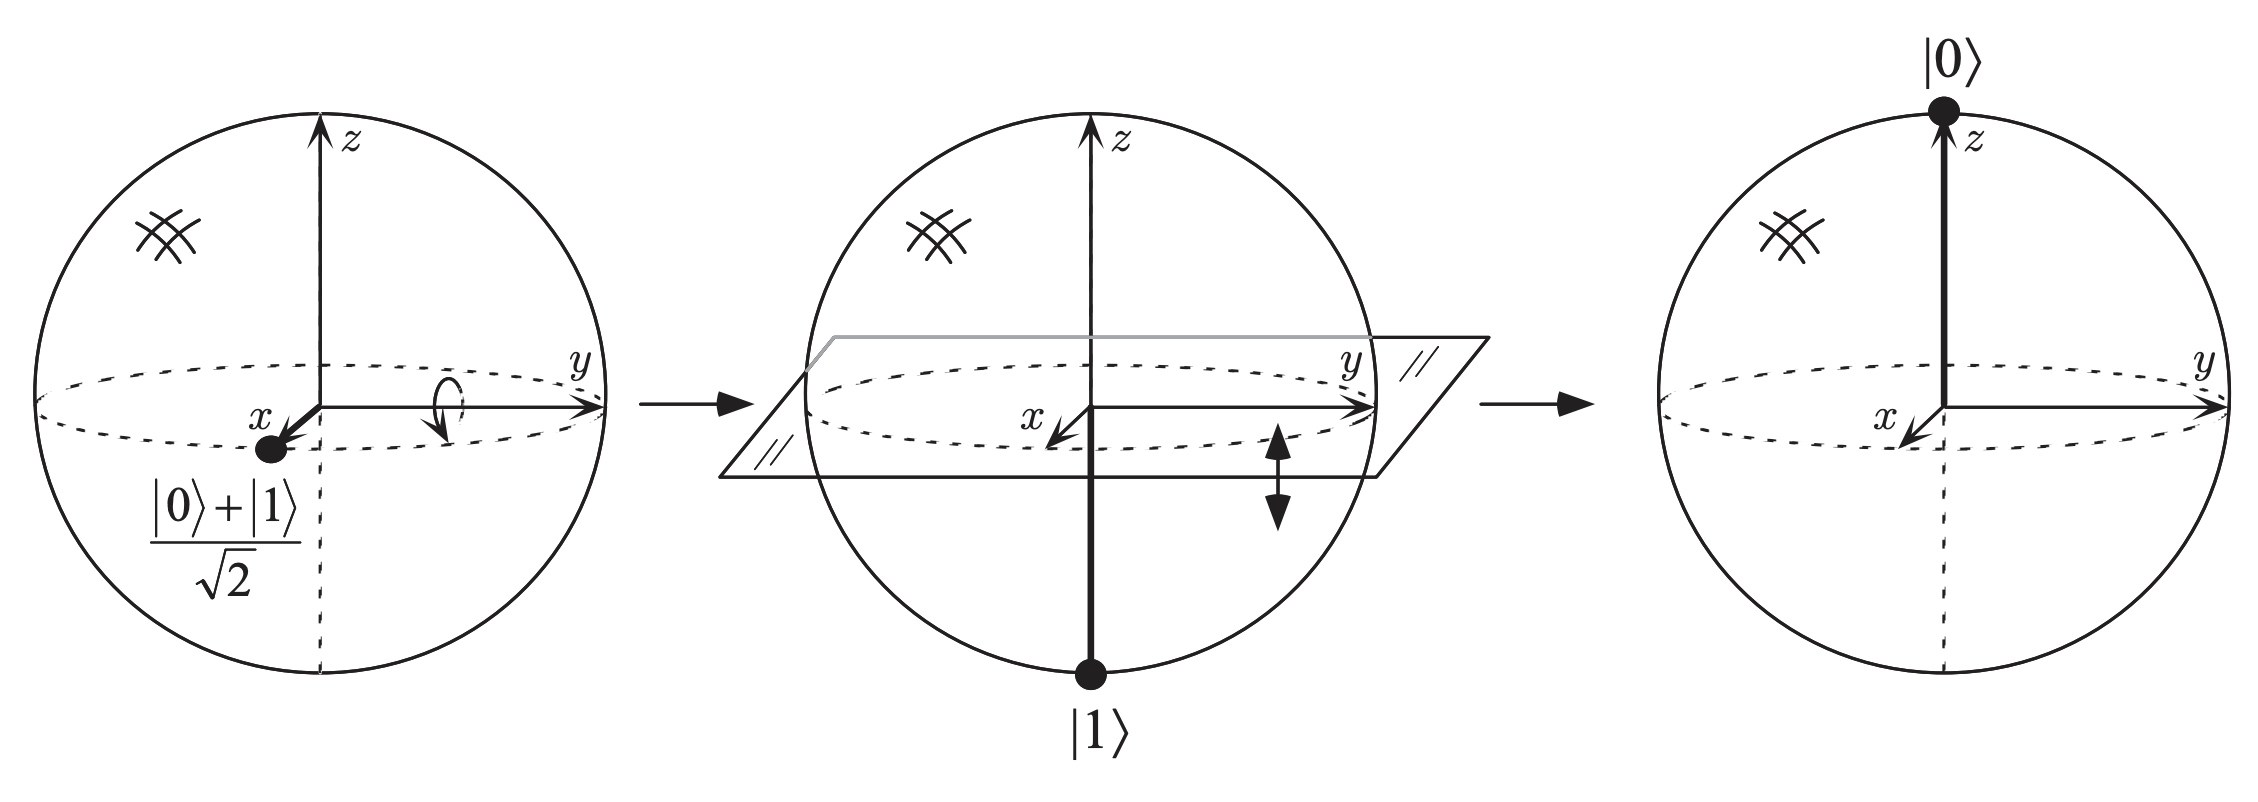
\includegraphics[width=\textwidth]{figures/hadamard}
  \caption[Hadamard Visualization]{Visualization of the Hadamard gate on the Bloch sphere, acting on the $\Ket{+}$ state \cite{nielsen2002quantum}.}
\end{figure}

An overview of some common single-qubit gates is given in figure \ref{fig:singlegates}.

\begin{table}[H]
  \label{fig:singlegates}
  \centering
  \begin{tabular}{c c c}uu
    Operator & Gate & Matrix \\[20pt]
    $X$ &  \Qcircuit @C=1em @R=.7em { & \gate{X} & \qw } & $\begin{pmatrix} 0 & 1 \\ 1 & 0\end{pmatrix}$ \\[20pt]
    $Y$ &  \Qcircuit @C=1em @R=.7em { & \gate{Y} & \qw } & $\begin{pmatrix} 0 & -i \\ i & 0\end{pmatrix}$ \\[20pt]
    $Z$ &  \Qcircuit @C=1em @R=.7em { & \gate{Z} & \qw } & $\begin{pmatrix} 1 & 0 \\ 0 & -1\end{pmatrix}$ \\[20pt]
    $H$ &  \Qcircuit @C=1em @R=.7em { & \gate{H} & \qw } & $\frac{1}{\sqrt{2}} \begin{pmatrix} 1 & 1 \\ 1 & -1\end{pmatrix}$ \\[20pt]
    $S$ &  \Qcircuit @C=1em @R=.7em { & \gate{S} & \qw } & $\begin{pmatrix} 1 & 0 \\ 0 & i\end{pmatrix}$ \\[20pt]
    $T$ &  \Qcircuit @C=1em @R=.7em { & \gate{T} & \qw } & $\begin{pmatrix} 1 & 0 \\ 0 & e^{i\frac{\pi}{2}}\end{pmatrix}$ \\[20pt]
  \end{tabular}
  \caption[Overview of common single-qubit gates]{Overview of common single-qubit gates.}
\end{table}

There are indefinitely many possible quantum gates in theory. Still, 
a universal finite gate set 
consisting of a few gates is sufficient to construct arbitrary unitary
transformations \cite{kitaev2002classical}. This is the same as in the classical case where NAND gates
suffice to build up arbitrary classical computation circuits \cite{sheffer13transactions} and 
 good news for the fabrication of quantum computers with reusable components.

Nevertheless, single-qubit gates are not sufficient to build all possible unitary transformations on multi-qubit systems. 
For this purpose, multi-qubit gates are a necessity.

\subsection{Multi-Qubit Gates}

Single-qubit gates are not sufficient to create universal gate sets for quantum
computation. In order to run arbitrary quantum programs, multi-qubit gates like
 \textit{controlled} gates are needed.
Controlled quantum gates are simple extensions of single-qubit gates. Every single-qubit gate can be implemented as a controlled 
version of it with one \textit{control} and one \textit{target} qubit. Only if
the control qubit is in the $\Ket{1}$ state, the gate is applied to the target
qubit. As the control qubit can be in a superposition state, it is possible to apply and not apply the gate to the target qubit at the same time.

The prototypical two-qubit gate is the controlled NOT or CNOT gate. It is the controlled version of the 
$X$ gate described before. As the CNOT gate acts on a two-qubit state, it can be described by 
a $4 \times 4$ unitary matrix. Each column describes the mapping of one of the four base
state $\Ket{00}$, $\Ket{01}$, $\Ket{10}$ and $\Ket{11}$. 
The matrix representation of the CNOT gate is the following:

\begin{equation}
  CNOT = \begin{pmatrix}
    1 & 0 & 0 & 0 \\
    0 & 1 & 0 & 0 \\
    0 & 0 & 0 & 1 \\
    0 & 0 & 1 & 0
    \end{pmatrix}.
\end{equation}

The matrix can be read as follows: The first two columns describe that the vectors $\Ket{00}$ and $\Ket{01}$ will not change when the gate is applied to these states. Only when the first qubit is in the $\Ket{1}$ state, will the state of the second qubit be swapped. Thus $\Ket{10}$ will be mapped to $\Ket{11}$ and $\Ket{11}$ to $\Ket{10}$. 

This shows how the matrix representation of generalized two-qubit gates can be derived: As long as the control qubit is off, it does not affect the state. Thus, the controlled gate matrix is the same as the identity with 1s on the diagonal and 0s elsewhere in the upper left corner. Only when the first qubit is in the $\Ket{1}$ state, the matrix differs from the identity. For example, the 
controlled version of the $Z$ gate:

\begin{equation}
  Z = \begin{pmatrix}
    1 & 0 \\
    0 & -1
    \end{pmatrix}
\end{equation}

is given by:

\begin{equation}
    CZ = \begin{pmatrix}
      1 & 0 & 0 & 0 \\
      0 & 1 & 0 & 0 \\
      0 & 0 & 1 & 0 \\
      0 & 0 & 0 & -1
      \end{pmatrix}.
\end{equation}

A controlled gate $G$ is represented by a vertical line ending in a black dot
indicating the control qubit:

\begin{figure}[h]
  \centering
  \mbox{
    \Qcircuit @C=1em @R=1em {
      &  \ctrl{1} & \qw \\
      &  \gate{G} & \qw
    }
  }
\end{figure}

With two-qubit operations at hand, it is possible to build a universal gate set. A commonly used gate set 
is the so-called \textit{Clifford + T} set, consisting of the gates $CNOT$, $H$, $S$ and
$T$ \cite{gottesman1998heisenberg}. The Solovay-Kitaev theorem \cite{kitaev2002classical} guarantees that this set can efficiently
approximate any unitary operation. In this study, another universal gate set will be used, 
composed of the $CZ$, $\sqrt{X}$, $\sqrt{Y}$ and $T$ gates \cite{martines2019supremacy}.

\section{Quantum Circuits}

The standard model for computation in theoretical computer science is the Turing Machine \cite{10.1112/plms/s2-42.1.230}. Invented by 
Alan Turing in 1936, it is a powerful tool to understand the limits of (classical) 
computation. The
theoretical nature of the Turing machine gives it unlimited computational
resources, like infinite memory, which do not reflect the properties of realizable
computer architectures.

Another computation model that does not suffer from the gap between theory
and practice is the \textit{circuit model} \cite{10.5555/522806}. In the classical circuit model, each bit is represented by a wire, and operations (or gates) are represented by different shapes acting on those wires. The circuit model is as powerful as a Turing Machine. It is the model of choice in quantum computing.

Quantum programs are described by quantum circuits. Each qubit is represented 
by a wire and each gate by a rectangular on those wires. Figure~\ref{fig:circuit0} describes a very simple quantum circuit which flips a single
qubit initialized in the $\Ket{0}$ state by applying a $X$ gate before
measuring it.

\begin{figure}[h]
  \centering
  \mbox{
    \Qcircuit @C=1em @R=1em {
      &  \lstick{\Ket{0}} & \qw & \gate{X} & \qw & \meter{0/1} 
    }
  }
  \label{fig:circuit0}
  \caption[A Simple Quantum Circuit]{A simple quantum circuit applying an $X$ gate to a qubit initialized in the $\Ket{0}$ state before measuring it.}
\end{figure}

The circuit is being read from left to right. Important to note is that
for calculating the resulting state, the matrix representation of the
gates are multiplied from the left side to the current state $\Ket{\psi}$
In the example above the final state of the program represented at the end of the circuit is:

\begin{align}
  \Ket{\phi} &= X \Ket{\psi} \\
             &=
               \begin{pmatrix}
                 0 & 1 \\
                 1 & 0
               \end{pmatrix}
                     \Ket{\psi} \\
             &= \begin{pmatrix}
               0 & 1 \\
               1 & 0
             \end{pmatrix}
                   \begin{pmatrix}
                     \alpha \\
                     \beta
                   \end{pmatrix} \\
             &= \begin{pmatrix}
               \beta \\
               \alpha
             \end{pmatrix}.
\end{align}

In practice, circuits consist of several qubits and multiple gates, that are applied
to them. It is possible to apply gates to different qubits sequentially as well
as in parallel, as demonstrated in figure~\ref{fig:circuit1}:

\begin{figure}[H]
  \centering
  \mbox{
    \Qcircuit @C=1em @R=1em {
      & \lstick{\Ket{0}} & \gate{H} & \gate{Z} & \qw & \gate{H} & \qw & \meter{0/1} \\
      & \lstick{\Ket{0}} & \qw & \gate{X} & \qw & \ctrl{-1} & \qw & \meter{0/1}
    }
  }
  \label{fig:circuit1}
  \caption[A Quantum Circuit Acting on two Qubits]{A quantum circuit acting on two qubits. The effect of parallel applications of single-qubit gates is defined by the tensor product of the gates.}
\end{figure}

Note that, when calculating the state of the quantum program above, the state of the system 
is given by the tensor product of the individual qubit states.
For the circuit from figure \ref{fig:circuit1}, the initial state $\Ket{\psi_{init}}$ before any gate has been applied 
is:

\begin{align}
    \Ket{\psi_{init}} &= \Ket{0} \otimes \Ket{0} \\
                      &= \begin{pmatrix} 1 \\ 0 \end{pmatrix} \otimes \begin{pmatrix} 1 \\ 0 \end{pmatrix} \\
                      &= \begin{pmatrix} 1 \\ 0 \\ 0 \\ 0 \end{pmatrix} \\
                      &= \Ket{00}. 
\end{align}

When a gate gets applied to only a subset of the qubits, as in the case of the
first $H$ gate in the circuit above, the unitary applied to the multi-qubit state is
implicitly the tensor product of the gate on that qubit and identity matrices on the
remaining qubits. For the given circuit, the state $\Ket{\psi_{H_1}}$ after the
first $H$ gate on the first qubit is calculated as: 

\begin{align}
  \Ket{\psi_{H_1}}  &= (H \otimes I) \Ket{00} \\
                   &= \left(\frac{1}{\sqrt{2}} \begin{pmatrix} 1 & 1 \\ 1 & -1 \end{pmatrix} \otimes \begin{pmatrix} 1 & 0 \\ 0 & 1 \end{pmatrix}\right) \Ket{00} \\
                    &= \frac{1}{\sqrt{2}} \begin{pmatrix} 1 & 0 & 1 & 0 \\ 0 & 1 & 0 & 1 \\ 1 & 0 & -1 & 0 \\ 0 & 1 & 0 & -1 \end{pmatrix} \Ket{00} \\
                    &= \frac{1}{\sqrt{2}} \begin{pmatrix} 1 & 0 & 1 & 0 \\ 0 & 1 & 0 & 1 \\ 1 & 0 & -1 & 0 \\ 0 & 1 & 0 & -1 \end{pmatrix} \begin{pmatrix} 1 \\ 0 \\ 0 \\ 0 \end{pmatrix} \\
                    &= \frac{1}{\sqrt{2}} \begin{pmatrix} 1 \\ 0 \\ 1 \\ 0 \end{pmatrix} \\
                    &= \Ket{+0}.
\end{align}

As expected, applying a $H$ gate to the first
qubit, it should be in the $\Ket{+}$ state while the second qubit remains in
the $\Ket{0}$ state.

Similar to the first gate, the unitary applied to the state, when multiple
gates are applied to different qubits at the same time, is constructed by the
tensor product of those gates. The resulting state $\Ket{\psi_{Z_1X_2}}$ after the $Z$
gate is applied to the first qubit, and the $X$ gate is applied to the second qubit, is
calculated as:

\begin{align}
  \Ket{\psi_{Z_1X_2}}  &= (Z \otimes X) \Ket{+0} \\
                    &= \left(\begin{pmatrix} 1 & 0 \\ 0 & -1 \end{pmatrix} \otimes \begin{pmatrix} 0 & 1 \\ 1 & 0 \end{pmatrix}\right) \Ket{+0} \\
                    &= \begin{pmatrix} 0 & 1 & 0 & 0 \\ 1 & 0 & 0 & 0 \\ 0 & 0 & 0 & -1 \\ 0 & 0 & -1 & 0 \end{pmatrix} \Ket{+0} \\
                    &= \begin{pmatrix} 0 & 1 & 0 & 0 \\ 1 & 0 & 0 & 0 \\ 0 & 0 & 0 & -1 \\ 0 & 0 & -1 & 0 \end{pmatrix} \begin{pmatrix} \frac{1}{\sqrt{2}} \\ 0 \\ \frac{1}{\sqrt{2}} \\ 0 \end{pmatrix} \\
                    &= \begin{pmatrix} 0 \\ \frac{1}{\sqrt{2}} \\ 0 \\ -\frac{1}{\sqrt{2}} \end{pmatrix} \\
                    &= \Ket{-1}.
\end{align}

Accordingly, applying a $Z$ gate to the $\Ket{+}$
state brings the first qubit to the $\Ket{-}$ state, while the $X$ gate on the second qubit moves the qubit state from the $\Ket{0}$ to the $\Ket{1}$ state.

The final state $\Ket{\psi_{final}}$ of the circuit is calculated by applying the $4 \times 4$ matrix
representation of the controlled $H$ gate to $\Ket{-1}$. In this case, the second
qubit is the controlled qubit:

\begin{align}
  \Ket{\psi_{final}}    &= CH \Ket{-1} \\
                        &= \begin{pmatrix} 1 & 0 & 0 & 0 \\ 0 & \frac{1}{\sqrt{2}} & 0 & \frac{1}{\sqrt{2}} \\ 0 & 0 & 1 & 0 \\ 0 & \frac{1}{\sqrt{2}} & 0 & -\frac{1}{\sqrt{2}} \end{pmatrix} \Ket{-1} \\
                       &= \begin{pmatrix} 1 & 0 & 0 & 0 \\ 0 & \frac{1}{\sqrt{2}} & 0 & \frac{1}{\sqrt{2}} \\ 0 & 0 & 1 & 0 \\ 0 & \frac{1}{\sqrt{2}} & 0 &  -\frac{1}{\sqrt{2}} \end{pmatrix} \begin{pmatrix} 0 \\ \frac{1}{\sqrt{2}} \\ 0 \\ -\frac{1}{\sqrt{2}} \end{pmatrix} \\
                       &= \begin{pmatrix} 0 \\ 0 \\ 0 \\ 1 \end{pmatrix} \\
                       &= \Ket{11}.
\end{align}

The first qubit has been swapped from the $\Ket{-}$ to the $\Ket{1}$ state as the
second qubit is in the $\Ket{1}$ state and the $H$ gate has been applied.
The circuit \ref{fig:circuit1} thus maps the initial state $\Ket{00}$ to $\Ket{11}$.

Another simple quantum circuit, which entangles two qubits with each other, is shown in figure \ref{fig:circuit2}.

\begin{figure}[H]
  \centering
  \mbox{
    \Qcircuit @C=1em @R=1em {
      & \lstick{\Ket{0}} & \gate{H} & \ctrl{1} & \qw & \meter{0/1} \\
      & \lstick{\Ket{0}} & \qw & \targ & \qw & \meter{0/1}
    }
  }
  \label{fig:circuit2}
  \caption[Bell State Creation Circuit]{A quantum circuit to create maximally entangled 2-qubit states.}
\end{figure}

The Hadamard gate on the first qubit maps the system from the initial $\Ket{00}$
into the $\Ket{+0}$ state. Afterward, the first qubit, which is currently
between the $\Ket{0}$ and $\Ket{1}$ state on the Bloch Sphere, is used as the
control qubit in the $CNOT$ gate. This has an interesting effect on the second qubit,
as the $X$ gate is applied and not applied at the same time, entangling
the two qubits with each other. The final state before measurement is
$\frac{\Ket{00} + \Ket{11}}{2}$, which has been discussed in section~\ref{sec:multiplequbitsandentanglement}.
This state is also known as one of the four \textit{Bell states}. They represent maximally
entangled two-qubit states. Moreover, they play an important role in the analysis of
\textit{quantum communication}.

The quantum circuit demonstrates how entanglement can be created by applying controlled gates with qubits in superposition states.
Entanglement plays an essential role in the construction of so-called \textit{random
quantum circuits} in recent quantum supremacy experiments.


\section{Quantum Computational Complexity}

It is essential to understand the theoretical capabilities and limitations of quantum computers to understand for which kind of problems
they provide advantages over classical computers. 

For many years, it has been assumed that the extended Church Turing thesis holds true. It states that a probabilistic
Turing machine can efficiently simulate any realistic model of computation. The thesis is challenged by quantum computers, because they can potentially solve specific problems exponentially faster than classical computers \cite{feynman1982simulating}.

The class of problems which can be solved efficiently by a quantum
computer is called \textbf{BQP}, shorthand for \textit{bounded-error quantum
  polynomial time} \cite{Bernstein93quantumcomplexity}. A decision problem is in \textbf{BQP} if there exists a quantum
program that solves the decision problem in 2/3 of the cases and runs in
polynomial time. This is the quantum analog of the \textit{bounded-error
  probabilistic polynomial time} or \textbf{BPP} \cite{gill1977computational}, which is decidable by a
probabilistic Turing machine in polynomial time and widely believed to be the same as
\textbf{P}.

Currently, there are a few problems known to be in \textbf{BQP}, which are suspected not to be in \textbf{P}, providing evidence for the superiority of quantum computers. One
of these problems is \textit{factorization}, the problem of decomposing a
composite integer into its prime factors. This problem has been known to be in
\textit{NP} before. Though, it is also known that factorization is not an \textbf{NP}-hard problem, indicating that quantum computers are not able to provide
an exponential speedup for every problem that is not efficiently solvable on a
classical computer. Indeed, classical algorithms might even exist, which can
solve factorization on a classical computer efficiently, which have not been
discovered yet.

While \textbf{BQP} includes \textbf{P} and intersects with \textbf{NP}, it can be shown that it is strictly
included in \textbf{PSPACE} \cite{Bernstein93quantumcomplexity}. The relationship of these complexity classes is visualized
in figure \ref{fig:complexityclasses}.

\begin{figure}[H]
  \centering
  \begin{tikzpicture}

    \draw[line width=0.5mm] (orig) circle (1.25);
    \draw[dashed, line width=0.5mm] (orig) ellipse (2.05 and 1.35);
    \draw[line width=0.5mm] (0,0.5) circle (2);
    \draw[line width=0.5mm] (0,1) circle (2.5);

    \draw (0,0) node {\large \textbf{P}};
    \draw (0,2) node {\large \textbf{NP}};
    \draw (0,2.9) node {\large \textbf{PSPACE}};
    \draw (2.5,-1) node {\large \textbf{BQP?}};

  \end{tikzpicture}
  \caption[Relation of Complexity Classes to each other]{Relation of Complexity Classes to each other.}
  \label{fig:complexityclasses}
\end{figure}

While it is hard to prove some fundamental relationships between complexity
classes like the famous $\mathbf{P} \stackrel{?}{=} \mathbf{NP}$ problem, it is believed that quantum computers
can solve specific problems with practical applications like integer factorization \cite{shor1997factorisation} or the simulation of
quantum systems \cite{feynman1982simulating} exponentially faster than classical computers.

The moment
in time a physical quantum computer can outperform a classical computer
on a specific problem for the first time has been coined by John Preskill in
2012 as \textit{quantum supremacy} \cite{preskill2012quantum}. Recently, Google announced their quantum
supremacy results with a 54 qubit quantum computer, providing the first physical evidence that it
might be possible to build quantum computers with advantages over classical
computers \cite{martines2019supremacy}.
\chapter{Random Circuit Sampling}

Despite four decades
of research in quantum computing, 
there was no physical proof of whether it would be possible to realize quantum computers
that have an advantage over classical ones. This only changed
recently, when a team from Google and the UCSB claimed to have demonstrated \textit{quantum supremacy}
with a 54 superconducting qubit quantum processor \cite{martines2019supremacy}. For this purpose, they
chose the problem of \textit{random circuit sampling}, a problem designed explicitly
as a quantum supremacy experiment \cite{Boixo2018supremacy}.

This chapter will motivate and introduce the theoretical framework of random circuit
sampling, also used as the benchmark for Restricted Boltzmann Machines in this
study. Further, the results of Google's quantum supremacy experiments will be discussed.

\section{Quantum Supremacy}

John Preskill has coined the term \textit{quantum supremacy} in 2012
\cite{preskill2012quantum}. It describes the point in time when a physical quantum computer
outperforms a classical computer on some task for the first time. The problem
solved by the quantum computer does not need to be useful. Its only purpose is
to prove that a quantum computer can be realized, which has an advantage over
classical computers on \textit{some} problem.

There exist different proposals for quantum supremacy
experiments \cite{shor1997factorisation, aaronson2013boson, Boixo2018supremacy}. Since quantum computers do not promise to outperform classical
computers on every problem, as discussed in section~\ref{sec:quantumcomplexity}, but only provide a
practical advantage for problems which lie in \textbf{BQP} and outside of
\textbf{P}, quantum supremacy experiments must be based upon a strong theoretical foundation \cite{Bernstein93quantumcomplexity}.

One way to demonstrate quantum supremacy would be to run Shor's
algorithm for integer factorization \cite{shor1997factorisation} on a physical quantum computer on some number which would not be feasible
to decompose with known classical algorithms on existing supercomputers \cite{martinlopez2011experimental}. The issue with this approach is that many
qubits are necessary to represent such numbers while today it is possible to
build quantum processors with about 50 qubits of reasonable quality \cite{martines2019supremacy}.

Another famous proposal for a quantum supremacy experiment is \textit{Boson Sampling} \cite{aaronson2013boson}, which is based on the
fact that calculating the permutant of a matrix is computationally hard.

The approach that a team from Google and UCSB took last year is called \textit{Random
  Circuit Sampling} (RCS) \cite{Boixo2018supremacy, martines2019supremacy}. In this approach, random quantum circuits of specific structures that create highly
entangled states are run on a quantum processor and are simulated classically. For
enough qubits and depth, performing the classical simulations would take years on the biggest existing supercomputers \cite{martines2019supremacy}. If the quantum computer can generate outputs
for such circuits which cannot be simulated classically anymore while their output can still be
verified to be correct, this would demonstrate quantum supremacy. 

A metric that
allows the verification on random circuit instances that cannot be simulated is
the \textit{cross entropy difference}.

\section{Cross Entropy Difference}

The challenge of quantum supremacy is that one has to be able to verify the
results of the quantum computer on instances which cannot be calculated
classically anymore. In the case of integer factorization, this is a simple task
as the test for the correctness consists of simple multiplications which can be
performed efficiently. Since integer factorization needs more qubits than
currently available in existing quantum computer hardware, other supremacy
experiments like RCS provide a framework to demonstrate quantum supremacy much
earlier.

The first observation to understand the concept of RCS is that every quantum
circuit acting on $n$ qubits can be described by a single $2^n$ dimensional
unitary matrix \cite{nielsen2002quantum}, as illustrated in figure~\ref{fig:circuitasunitary}. This follows
from the fact that quantum gates are described by unitary transformations and
the matrix product, as well as the tensor product of two unitaries, is a unitary again.

\begin{figure}[H]
  \begin{equation}
      \vcenter{
          \Qcircuit @C=1em @R=1em {
          & \ctrl{2} & \qw & \gate{H} & \ctrl{1} &
          \gate{H} & \qw \\
          & \qw & \ctrl{1} & \gate{H} & \targ &
          \gate{H} & \qw \\
          & \targ & \targ & \gate{Z} & \qw & \ctrl{-1} &
          \qw
        }
      }
      =
      \vcenter{
        \Qcircuit @C=1em @R=0em {
          & \multigate{2}{U} & \qw \\
          & \ghost{U} & \qw \\
          & \ghost{U} & \qw
        } 
      }
    \end{equation}
    \label{fig:circuitasunitary}
  \caption[Quantum Circuits as Unitaries]{Every Circuit can be described by one big unitary acting on $n$
    qubits. W.l.o.g. the resulting states corresponds to the first row of the
    unitary $U$.}
\end{figure}

A quantum circuit consisting of gates chosen uniformly at random
will act like a uniformly random unitary $U$ \cite{Boixo2018supremacy}. Since the input state of the circuit can be assumed to be
initialized in the $\Ket{0}^{\otimes n}$ state, the amplitudes of the final
quantum state of the circuit correspond to the first column of the random unitary $U$.

This column's entries are complex numbers with real and imaginary parts
distributed by an unbiased Gaussian with respect to the normalization constraints.
The output probabilities of the random circuit are given by
the squared norms of these entries.
They are thus distributed as the square of
a Gaussian which is an exponential distribution,
also known as a Porter-Thomas \cite{Porter1956Fluctuations}. So the probabilities $p(x_j) =
| \Braket{x_j | \psi_{RC}} | ^2$ to observe bitstrings $x_j \in \{x_j\}_{j=1}^N$ with
$N=2^n$ are distributed according to

\begin{equation}
  Pr(p) = e^{-Np}
\end{equation}

as visualized in figure~\ref{fig:porterthomas}.

\begin{figure}[H]
  \label{fig:porterthomas}
  \centering
  \begin{tikzpicture}
    \begin{axis}[
      xmin=0,
      ymin=0,
      xmax=1,
      ymax=1]
      \addplot[blue, domain=0:1, thick] {e^(-5*x)};
    \end{axis}
  \end{tikzpicture}
  \caption[Output Distribution of Random Quantum Circuits]{Distribution $P(p_{x_j})$ of output probabilities $p_{x_j}$ of a
    quantum circuit. The distribution $P(p_{x_j})=e^{-Np}$ is distributed as
    Porter-Thomas. A lot of output strings will have a low probability to be
    observed and a few output strings will dominate the observed outputs \cite{Boixo2018supremacy}.}
\end{figure}

As quantum computers suffer from decoherent noise \cite{Zeh:1970zz}, it is
important to understand if noisy quantum computers can still
outperform classical computers on the RCS task. Knowing that the outputs are
Porter-Thomas distributed will help with that.

The task is to understand how samples $S=\{x_1,\dots,x_m\}$ drawn from a perfect execution of
$U$ compare to a set $S^{\prime}=\{x_1^{\prime},\dots,x_m^{\prime}\}$ of samples drawn from a potentially noisy
execution of $U$.

A well motivated measure for the difference between the underlying
probability distributions $p_U$ and $p_U^{\prime}$ of samples $S$ and $S^{\prime}$ is the \textit{cross entropy} \cite{kullback1951}, defined as


\begin{equation}
  H(p_U^{\prime},p_U) = - \sum_{j=1}^Np_U^{\prime}(x_j|U) \log{p_U(x_j)}.
\end{equation}

Of interest is the expected quality of the potentially noisy execution over
different random circuit instances:

\begin{align}
  \label{eq:expectedCrossDifference}
  \mathbb{E}_U[H(p_U^{\prime},p_U)] &= -\mathbb{E}_U[\log{p_U(x_j)}]
                                    &= \mathbb{E} \left[\sum_{j=1}^Np_U^{\prime}(x_j|U)\log{\frac{1}{p_U(x_j)}}\right]
\end{align}

The output of the noisy execution can be assumed to
be statistically uncorrelated with the output of the perfect execution \cite{Boixo2018supremacy}. Thus,
and since the output distribution for a fixed $x_j$ over many random circuit
instances $U$ also has the shape of the Porter-Thomas distribution \cite{harrow2008random},
$\mathbb{E}_U[\log{\frac{1}{p_U(x_j)}}] = -\mathbb{E}_U[\log{p_U(x_j)}]$ from equation~\ref{eq:expectedCrossDifference}can be computed independently as:

\begin{align}
  -\mathbb{E}_U[\log{p_U(x_j)}] &\approx - \int_0^{\infty}Ne^{-NP}\log{p} \,dp \\
                                &= \log{N} + \gamma,
\end{align}

where $\gamma \approx 0.577$ is the Euler constant.
Using the fact that $\sum_{j=1}^Np_U^{\prime}(x_j) = 1$ for any distribution $p_U{\prime}$, the average cross
entropy $\mathbb{E_U}[H(p_U^{\prime},p_U)]$ between the Porter-Thomas distribution and any other uncorrelated distribution is
given as 

\begin{equation}
  \mathbb{E}_U [H(p_U^{\prime},p_U)] = \log{N} + \gamma.
\end{equation}

This is equivalent to the cross entropy $H_0 = \log{N} + \gamma$ between the
Porter-Thomas and the uniform distribution. Thus, on
average, a worst-case noisy execution will be as good compared to a perfect execution as sampling
every bitstring with probability $1/N$. $H_0$ differs from the entropy $H(p_U)$ of
the Porter-Thomas distribution, which corresponds to the cross entropy with
itself, only by a $-1$ term:

\begin{align}
  H(p_U) &= - \int p N^2e^{-Np}\log{p} \, dp \\
         &= \log{N} -1 + \gamma,
\end{align}

This directly leads to a benchmark for any algorithm $A_U$ sampling output strings from a
random circuit $U$, given either by a
classical simulation or by a (noisy) quantum computer. The quality of 
$A_U$ can be calculated as the difference between
the entropy of the uniform distribution and the cross entropy of the output
samples from $A_U$ with the Porter-Thomas distribution. This metric is
defined as the \textit{cross entropy difference} \cite{Boixo2018supremacy}:

\begin{align}
  \Delta H(p_A) &\equiv H_0 - H(p_A, p_U) \\
                 &=\sum_j \left(\frac{1}{N} - p_A(x_j|U)\right)\log{\frac{1}{p_U(x_j)}}.
\end{align}

The cross entropy difference is zero for an algorithm sampling from the uniform
distribution and one for an algorithm sampling from the underlying Porter-Thomas
distribution of the circuit.

In order to calculate $\Delta H(p_A)$, 
a perfect simulation of the random circuit is necessary as the values of $p_U(x_j)$ have to be known. This is not possible in the quantum
supremacy regime. As discussed shortly, it will be possible
to extrapolate the cross entropy difference $\Delta H(p_A)$ of $A_U$ to the quantum supremacy regime with high
precision based on samples of its cross entropy difference on smaller circuit
instances which can still be simulated classically \cite{Boixo2018supremacy}.

Another justification for the cross entropy difference is that the $l_1$ distance between the uniform and Porter-Thomas distribution

\begin{align}
  l_1(p,q) &= \| p-q\|_1 \\
           &= \sum_{j=1}^N \mid p_i - q_i \mid
\end{align}

is $\frac{2}{e}$ and thus independent of the number of qubits $n$. Therefore, a
constant number of samples is sufficient to calculate the cross entropy $H(p_U)$
difference.

Experimentally, the cross entropy difference

\begin{equation}
  \alpha = \mathbb{E}_U[\Delta H(p^{\prime}_U)]
\end{equation}

can be obtained by the execution of several random circuits $U$. Quantum
supremacy is achieved by a physical quantum computer when its average cross
entropy

\begin{equation}
  1 \geq \alpha > C
\end{equation}

is greater than the average performance $C$ of the best known classical algorithm $A^*$:

\begin{equation}
  C = \mathbb{E}_U[\Delta H(p^*)] .
\end{equation}

In the regime where perfect simulations are possible, $C=1$ and quantum
supremacy cannot be achieved \cite{Boixo2018supremacy}. For sufficiently many qubits, perfect simulations
will not be possible anymore and $1 > C \geq 0$ with $C$ decreasing exponentially
with the number of gates $g>>n$. For a typical set of samples $S_{exp}$ drawn from the
execution of a quantum circuit, the central limit theorem implies that:

\begin{equation}
  \label{eq:cef}
  \alpha \simeq H_0 - \frac{1}{m} \sum_{j = 1}^m \log{\frac{1}{p_U(x_j^{exp})}}.
\end{equation}

The experimental setup to estimate the cross entropy difference of any
approximate simulation of a quantum computer thus is \cite{Boixo2018supremacy}:

\begin{enumerate}
\item Select random circuit $U$.
  \item Take sufficiently many samples $S_{exp} = \{x_1, \dots, x_m\}$, m in
    range $10^3-10^6$.
    \item Compute the quantities $\log{\frac{1}{p_U(x_j^{exp})}}$ with the aid
      of a sufficiently large classical computer.
      \item estimate $\alpha$ using equation~\ref{eq:cef}.
\end{enumerate}

\section{Extrapolating to the Supremacy Regime}

Keeping the qubits in a coherent state during a calculation and applying quantum
gates exactly is a difficult task \cite{martines2019supremacy}. Qubits will suffer from decoherent noise, which will destroy the quantum states. This will happen in particular in the early implementations of quantum computers.

Before large scale error-corrected quantum computers will be available, so-called noisy intermediate-scale quantum (NISQ) computers present the first stage
of quantum computing hardware. Such noisy devices will already provide an
advantage over classical computers on specific problems. If the noise can be
kept below a certain threshold, a NISQ device can demonstrate quantum
supremacy on the RCS task \cite{neill2018blueprint}.

In the presence of noise, the quantum state $\rho$ generated by a physical quantum computer
after the execution of a random circuit $U$ can be represented as

\begin{equation}
  \rho = \tilde{\alpha} U \Ket{\psi_0} \Bra{\psi_0} U^{\dagger} + (1- \tilde{\alpha}) \sigma
\end{equation}

with $\tilde{\alpha}$ being the circuit \textit{fidelity} and noise term $\sigma$ being an orthogonal state to the true state with
$\Bra{\psi_0}U^{\dagger}\sigma U \Ket{\psi_0} = 0$.
The corresponding average cross entropy difference is:

\begin{align}
  \alpha &= \mathbb{E}_U\left[H_0+ \sum_j \Bra{x_j} \rho \Ket{x_j} \log{p_U(x_j)} \right] \\
         &= \tilde{\alpha} + (1-\tilde{\alpha})H_0 + \mathbb{E}_U\left[(1-\tilde{\alpha}) \sum_j \Bra{x_j} \sigma \Ket{x_j} \log{p_U(x_j)}\right].
\end{align}

The states generated by the random circuits are
maximally entangled \cite{Boixo2018supremacy}. A single bit or phase flip introduced by an additional $ X $ or $ Z $ gate in the circuit completely destroys such a state. Instead of being Porter-Thomas distributed, the output would be almost uniformly distributed, as shown in figure~\ref{fig:rcs_noise}.

\begin{figure}[H]
  \centering
  \label{fig:rcs_noise}
  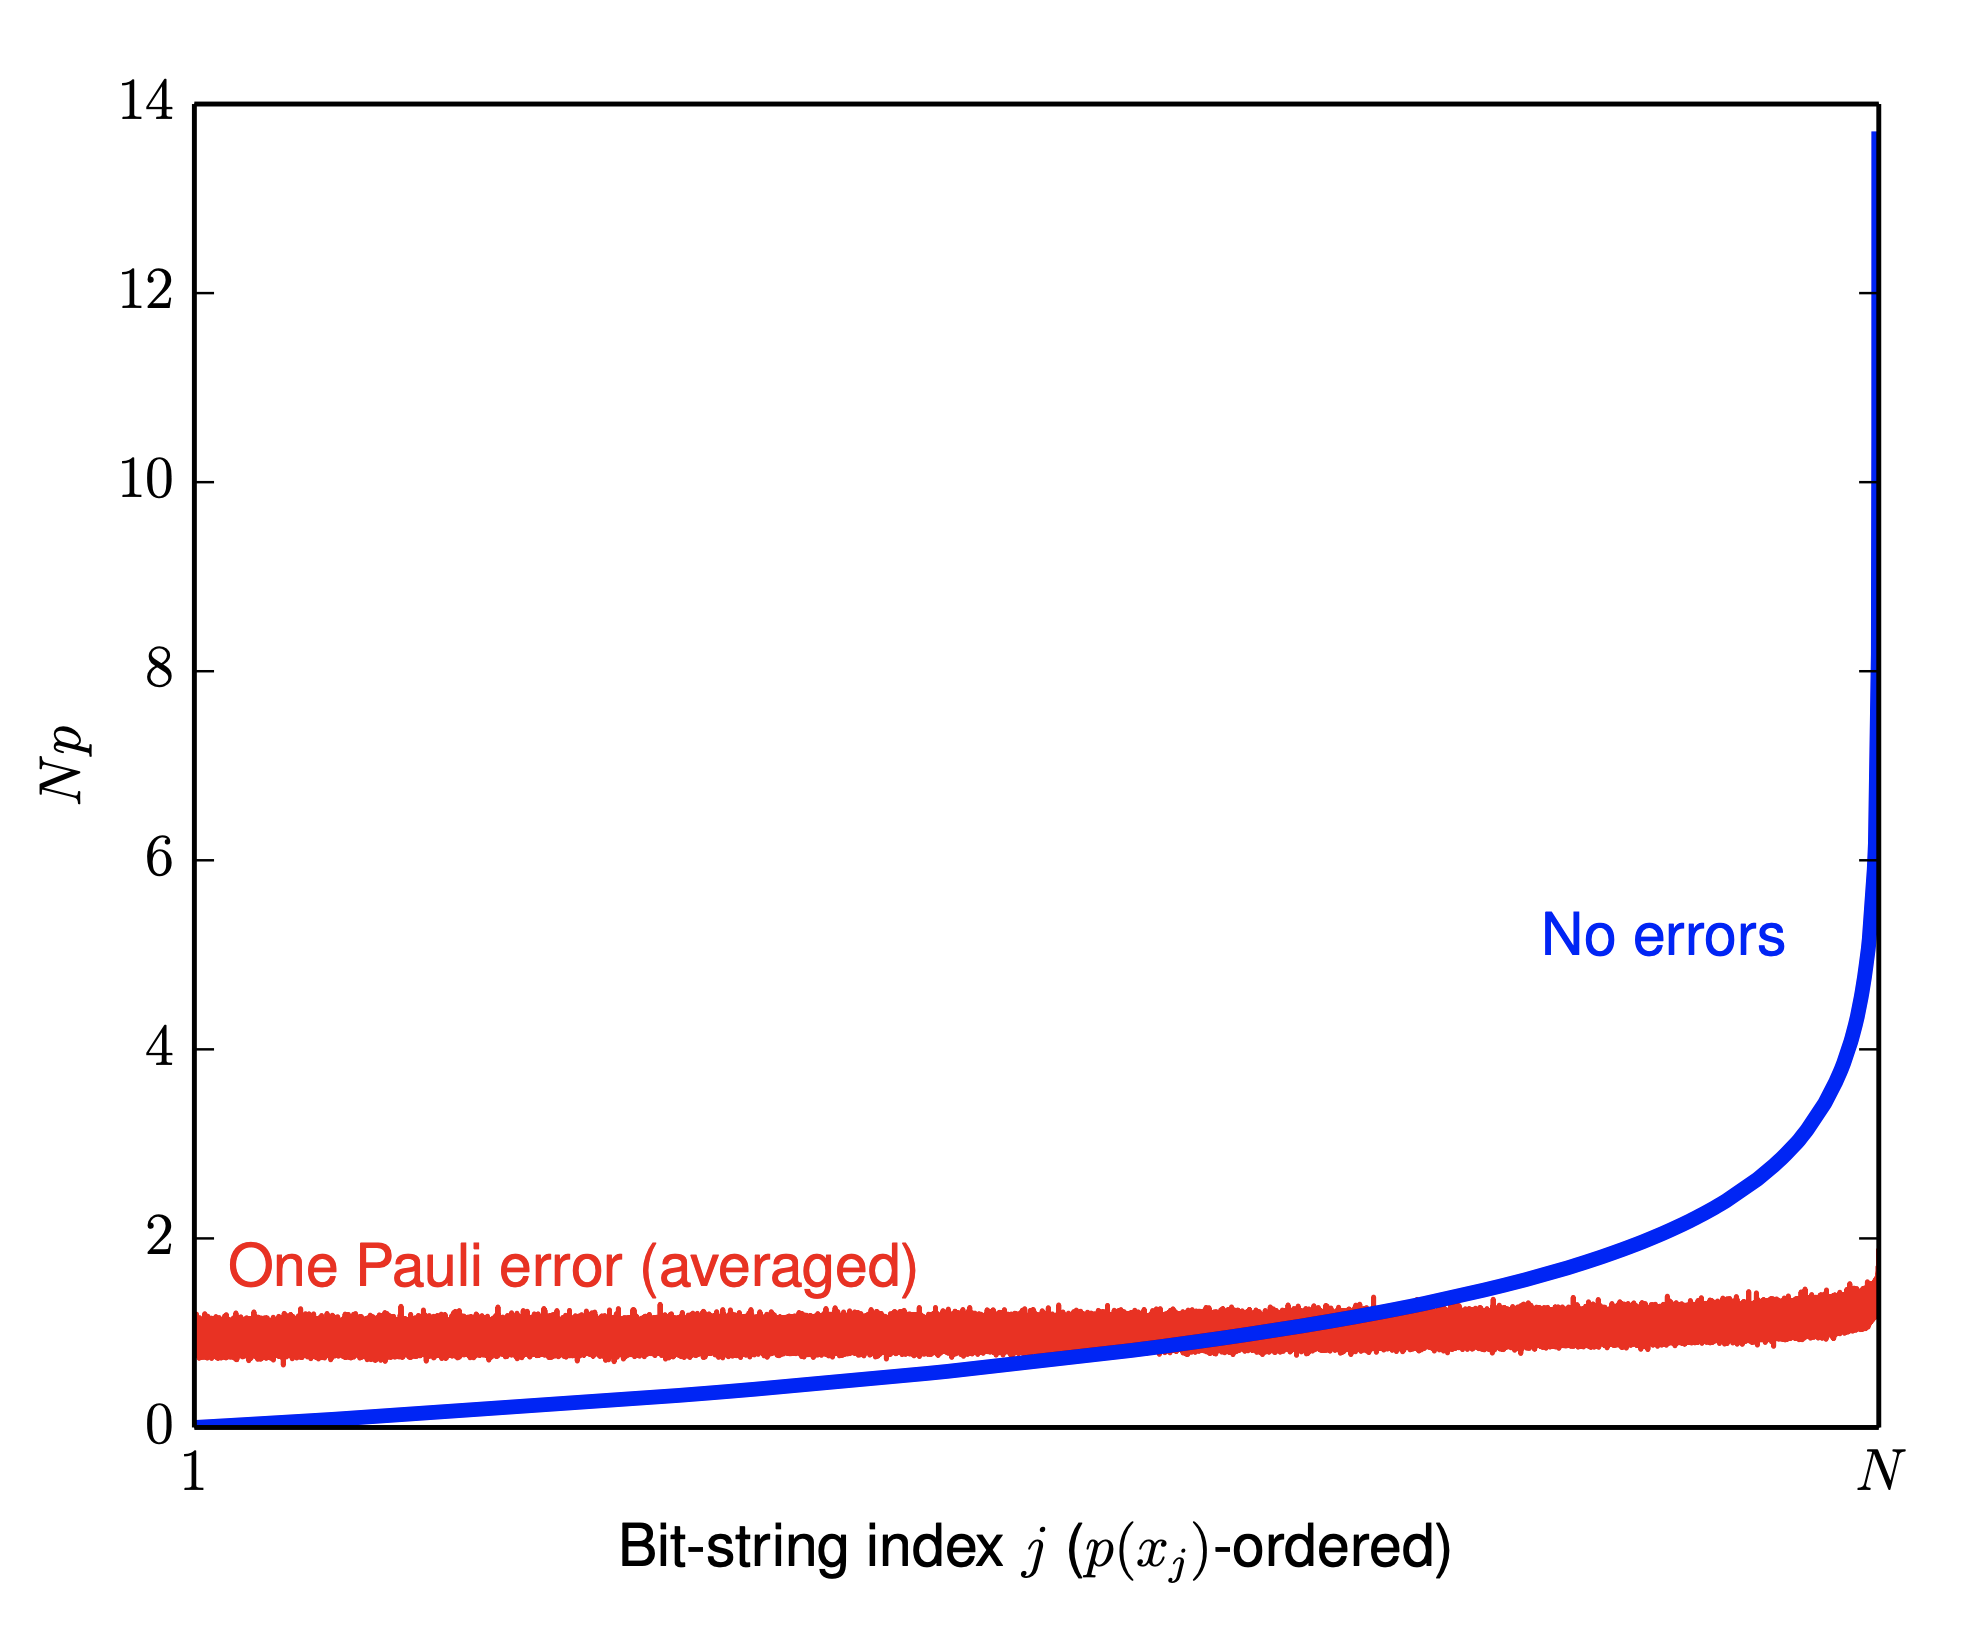
\includegraphics[width=0.58\textwidth]{figures/rcs_noise}
  \caption[Effect of one Pauli Error on Random Circuits]{Blue: Output bitstrings of a random circuit ordered by their probabilities. Red: Averaged 
  simulated output distribution with one Pauli error on all possible positions in a $5 \times 4$ qubits random circuit 
  with depth 40. The distribution is almost uniform and almost uncorrelated with the real output distribution. The small tild at 
  the end can be explained by the fact that Z gates close to the end of the circuit do not have an effect on the output distribution \cite{Boixo2018supremacy}.}
\end{figure}

In other words, it is not possible to infer any information about the output
probabilities without a perfect simulation of the circuit.
This justifies the assumption that the actual output probabilities and the output
of the quantum computer are (almost) uncorrelated.
This assumption of no correlation, in turn, leads to the conclusion that the
circuit fidelity $\tilde{\alpha}$ of a random
circuit $U$ is approximately equal to the average cross entropy:

\begin{equation}
  \label{eq:extrapolate}
  \alpha = \mathbb{E}_U[\Delta H(p_{exp})] \approx \tilde{\alpha}.
\end{equation}

This means that the fidelity $\alpha$ of a quantum device can be extrapolated to
the quantum supremacy regime from estimates on random circuit instances
which can still be simulated classically.

Even further, the cross entropy difference can also aid to estimate
the single and two-qubit gate and errors of a quantum device:

\begin{equation}
  \alpha \approx e^{-r_1g_1 - r_2g_2 -r_{init}n -r_{mes}n}
\end{equation}

with $r_1, r_2 \ll 1$ being the Pauli error rates for one and two-qubit gates, $r_{init},
r_{mes} \ll 1$ the initialisation and measurement error and $g_1,g_2 \gg 1$ being the
numbers of one and two-qubit gates. This relation has been numerically confirmed by
Boixo et al. \cite{Boixo2018supremacy}, indicating that the relation between the
cross entropy difference and the circuit fidelity can be used to extrapolate the
cross entropy difference of a quantum device to the quantum supremacy regime \cite{Boixo2018supremacy}.

So, even on the RCS task, a noisy quantum computer is able to demonstrate quantum
supremacy, by calculating the fidelity of the quantum computer on random circuit instances still possible to simulate
classically, which can be extrapolated to the supremacy regime using
equation~\ref{eq:extrapolate}.
If the fidelity is greater zero in the regime where no classical simulation is possible anymore,
quantum supremacy has been demonstrated \cite{Boixo2018supremacy}.

\section{Random Circuit Design}

The derivation of the cross entropy difference based on the assumption that the
output probabilities of random circuit instances will be distributed according to
the Porter-Thomas distribution \cite{Boixo2018supremacy}. As it is known that circuits of low depth as
well as so-called \textit{Clifford Circuits} can be simulated classically
efficiently \cite{gottesman1998heisenberg}, it is crucial to understand which requirements the structures of
the random circuits has to fulfill in order to be hard to simulate classically and generate
exponential output distributions \cite{Boixo2018supremacy}.

In a fully connected architecture, random circuits approximate a pseudo-random
distribution with logarithmic depth \cite{harrow2008random}. Fully connected in this statement means
that two-qubit gates can be applied to pairs of any two-qubits of the circuit. In
architectures like superconducting qubits such as Google's Sycamore
processor, the qubits are laid out on a 2D lattice, allowing two-qubit gates only
to be applied to neighboring qubits on that lattice \cite{barends2014logic}. Circuits on fully
connected architectures of logarithmic depths are known to be translatable into
circuits of depth $\sqrt{n}$ on 2D lattices \cite{beals2013efficient}. Boxio et al. used numerical
simulations to optimize strategies to generate random circuits with minimized
time to converge to a Porter-Thomas distribution, leading to the following algorithm \cite{Boixo2018supremacy}:

\begin{enumerate}
  \item Initialize in the state $\Ket{0}^{\otimes n}$.
  \item Apply a Hadamard gate to each qubit.
  \item Apply a random circuit with a stack of depth $d$, where each layer has
    the following two clock cycles:
    \begin{enumerate}
      \item Apply a clock cycle of random single-qubit gates to all qubits.
        \item Apply a clock cycle of two-qubits gates.
    \end{enumerate}
\end{enumerate}

The gate set consists of the single-qubit gates $\{\sqrt{X}, \sqrt{Y}, T\}$ with

\begin{equation}
  \sqrt{X} = \frac{1}{\sqrt{2}} \begin{pmatrix}
    1 & - i \\
    - i & 1
    \end{pmatrix}
\end{equation}

and

\begin{equation}
  \sqrt{Y} = \frac{1}{\sqrt{2}} \begin{pmatrix}
    1 & -1  \\
    1 & 1 
  \end{pmatrix}
\end{equation}

being the ``square root of $X$'' and the ``square root of $Y$'' gates:

\begin{align}
  \sqrt{X}^2 &= \left(\frac{1}{\sqrt{2}} \begin{pmatrix}
    1 & - i \\
    - i & 1
  \end{pmatrix}\right)^2 \\
  &= \begin{pmatrix}
    0 & 1 \\
    1 & 0
  \end{pmatrix} \\
  &= X
\end{align}

and

\begin{align}
  \sqrt{Y}^2 &= \left(\frac{1}{\sqrt{2}} \begin{pmatrix}
    1 & -1 \\
    1 & 1
  \end{pmatrix}\right)^2 \\
  &= \begin{pmatrix}
    0 & -i \\
    i & 0
  \end{pmatrix} \\
  &= Y.
\end{align}

The circuit can be separated into different layers, where each layer consists of one
layer of controlled $Z$ (CZ) gates and one layer of random single-qubit gates. The single-qubit
gates are chosen such that each single-qubit gate on qubit $q$ in the current
cycle differs from the single-qubit gate on $q$ at the previous cycle.

The two-qubit $CZ$ gates are applied as demonstrated in figure~\ref{fig:czgates}.

\begin{figure}[H]
  \centering
  \label{fig:czgates}
  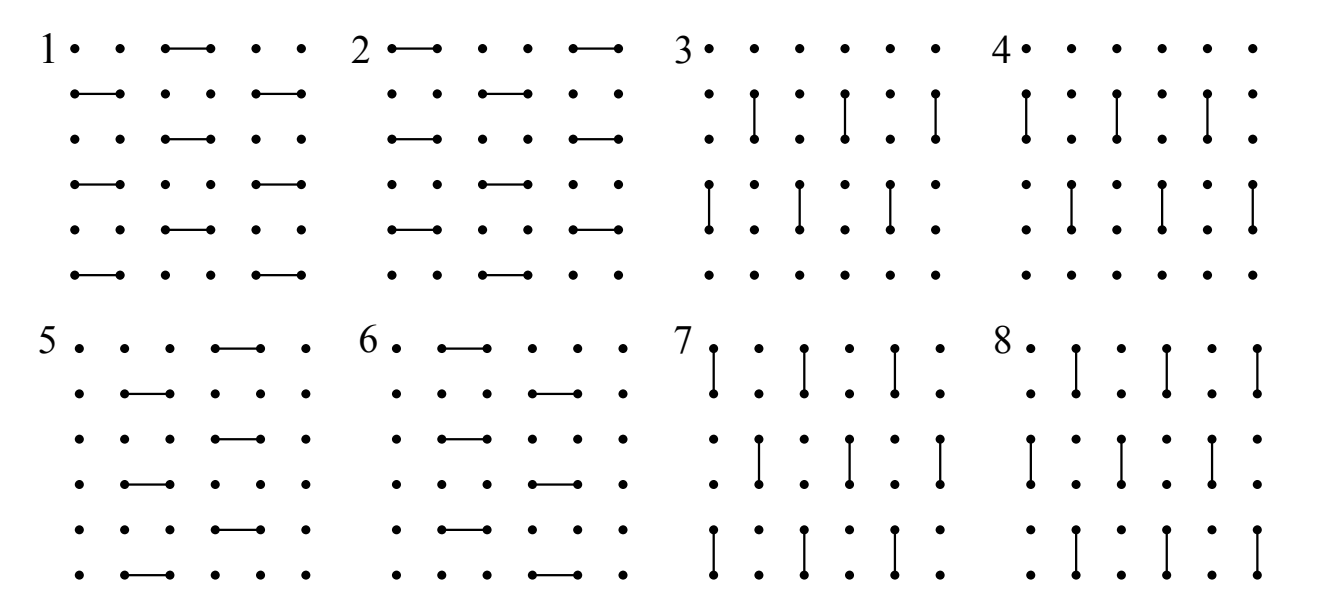
\includegraphics[width=0.58\textwidth]{figures/cz_order}
  \caption[Order of $CZ$ Gate Applications in Random Circuits]{Order in which $CZ$ gates are applied to the qubits. As 
  the qubits are aligned on a 2D lattice, only neighboring qubits can be coupled through $CZ$ gates. 
  The pattern repeats every 8 cycles.}
\end{figure}

Boxio et al. could numerically show that the output distribution of random circuits generated this way
converge to Porter-Thomas after a square root
number of cycles in the number of qubits \cite{Boixo2018supremacy}.

\section{Experiments the Sycamore Processor}

Built upon the theoretical framework of random circuit sampling,
a team from Google and the UCSB conducted a quantum
supremacy experiment on the 54 superconducting qubit \textit{Sycamore}
processor, shown in figure~\ref{fig:sycamore} \cite{martines2019supremacy}.

\begin{figure}[H]
  \centering
  \label{fig:sycamore}
  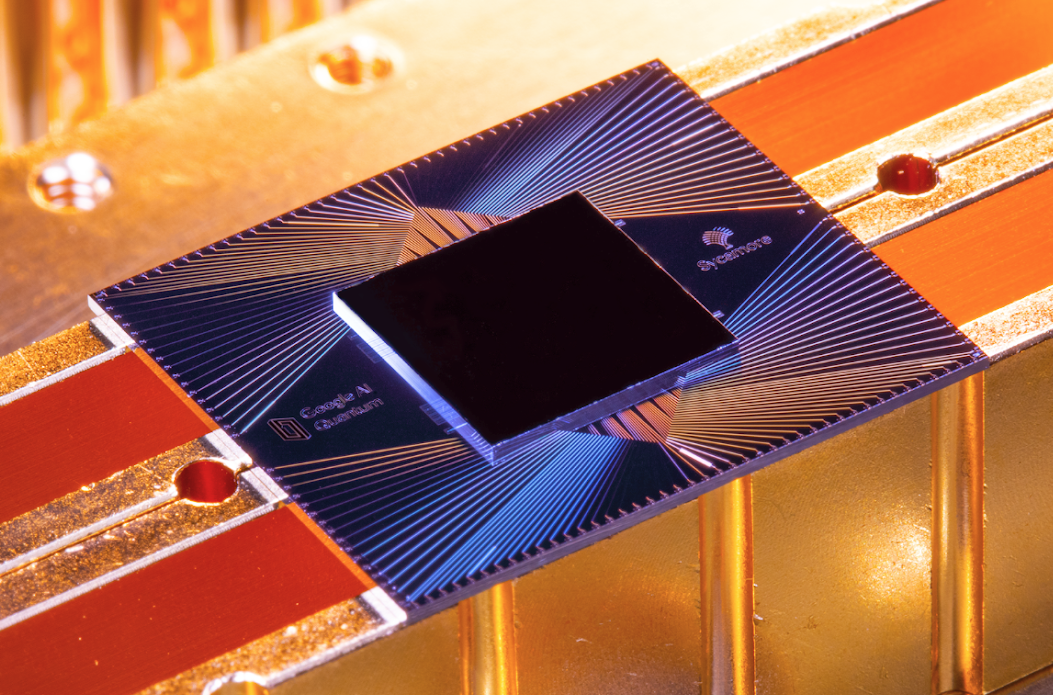
\includegraphics[width=0.58\textwidth]{figures/sycamore}
  \caption[The Sycamore processor]{The Sycamore processor used in the quantum supremacy experiments of Google and UCSB. It consists of 54 qubits of which one was malfunctioning \cite{martines2019supremacy}.}
\end{figure}

For the experiments, they generated circuits with $n=10$ to $n=53$ qubits and
$m=12$ to $m=20$ cycles. The full cycles generated according to the procedure
given above can be classically simulated up to $n=53$ qubits with $m=14$ cycles
in a reasonable amount of time. Beyond that regime, simplified circuit
architectures, called \textit{elided} and \textit{patched}, were used. These circuits
are split into two sub-circuits with only weak entanglement in the elided and no
entanglement in the patched version. Such circuits can be classically simulated for up to $n=53$ qubits with $m=20$ cycles to
verify the fidelity of the Sycamore processor. For every circuit parameters, 20
circuits have been generated. For each circuit, $0.5-2.5$ million samples have been drawn
from the quantum processor \cite{martines2019supremacy}.

\begin{figure}[H]
  \centering
  \label{fig:supremacy_results}
  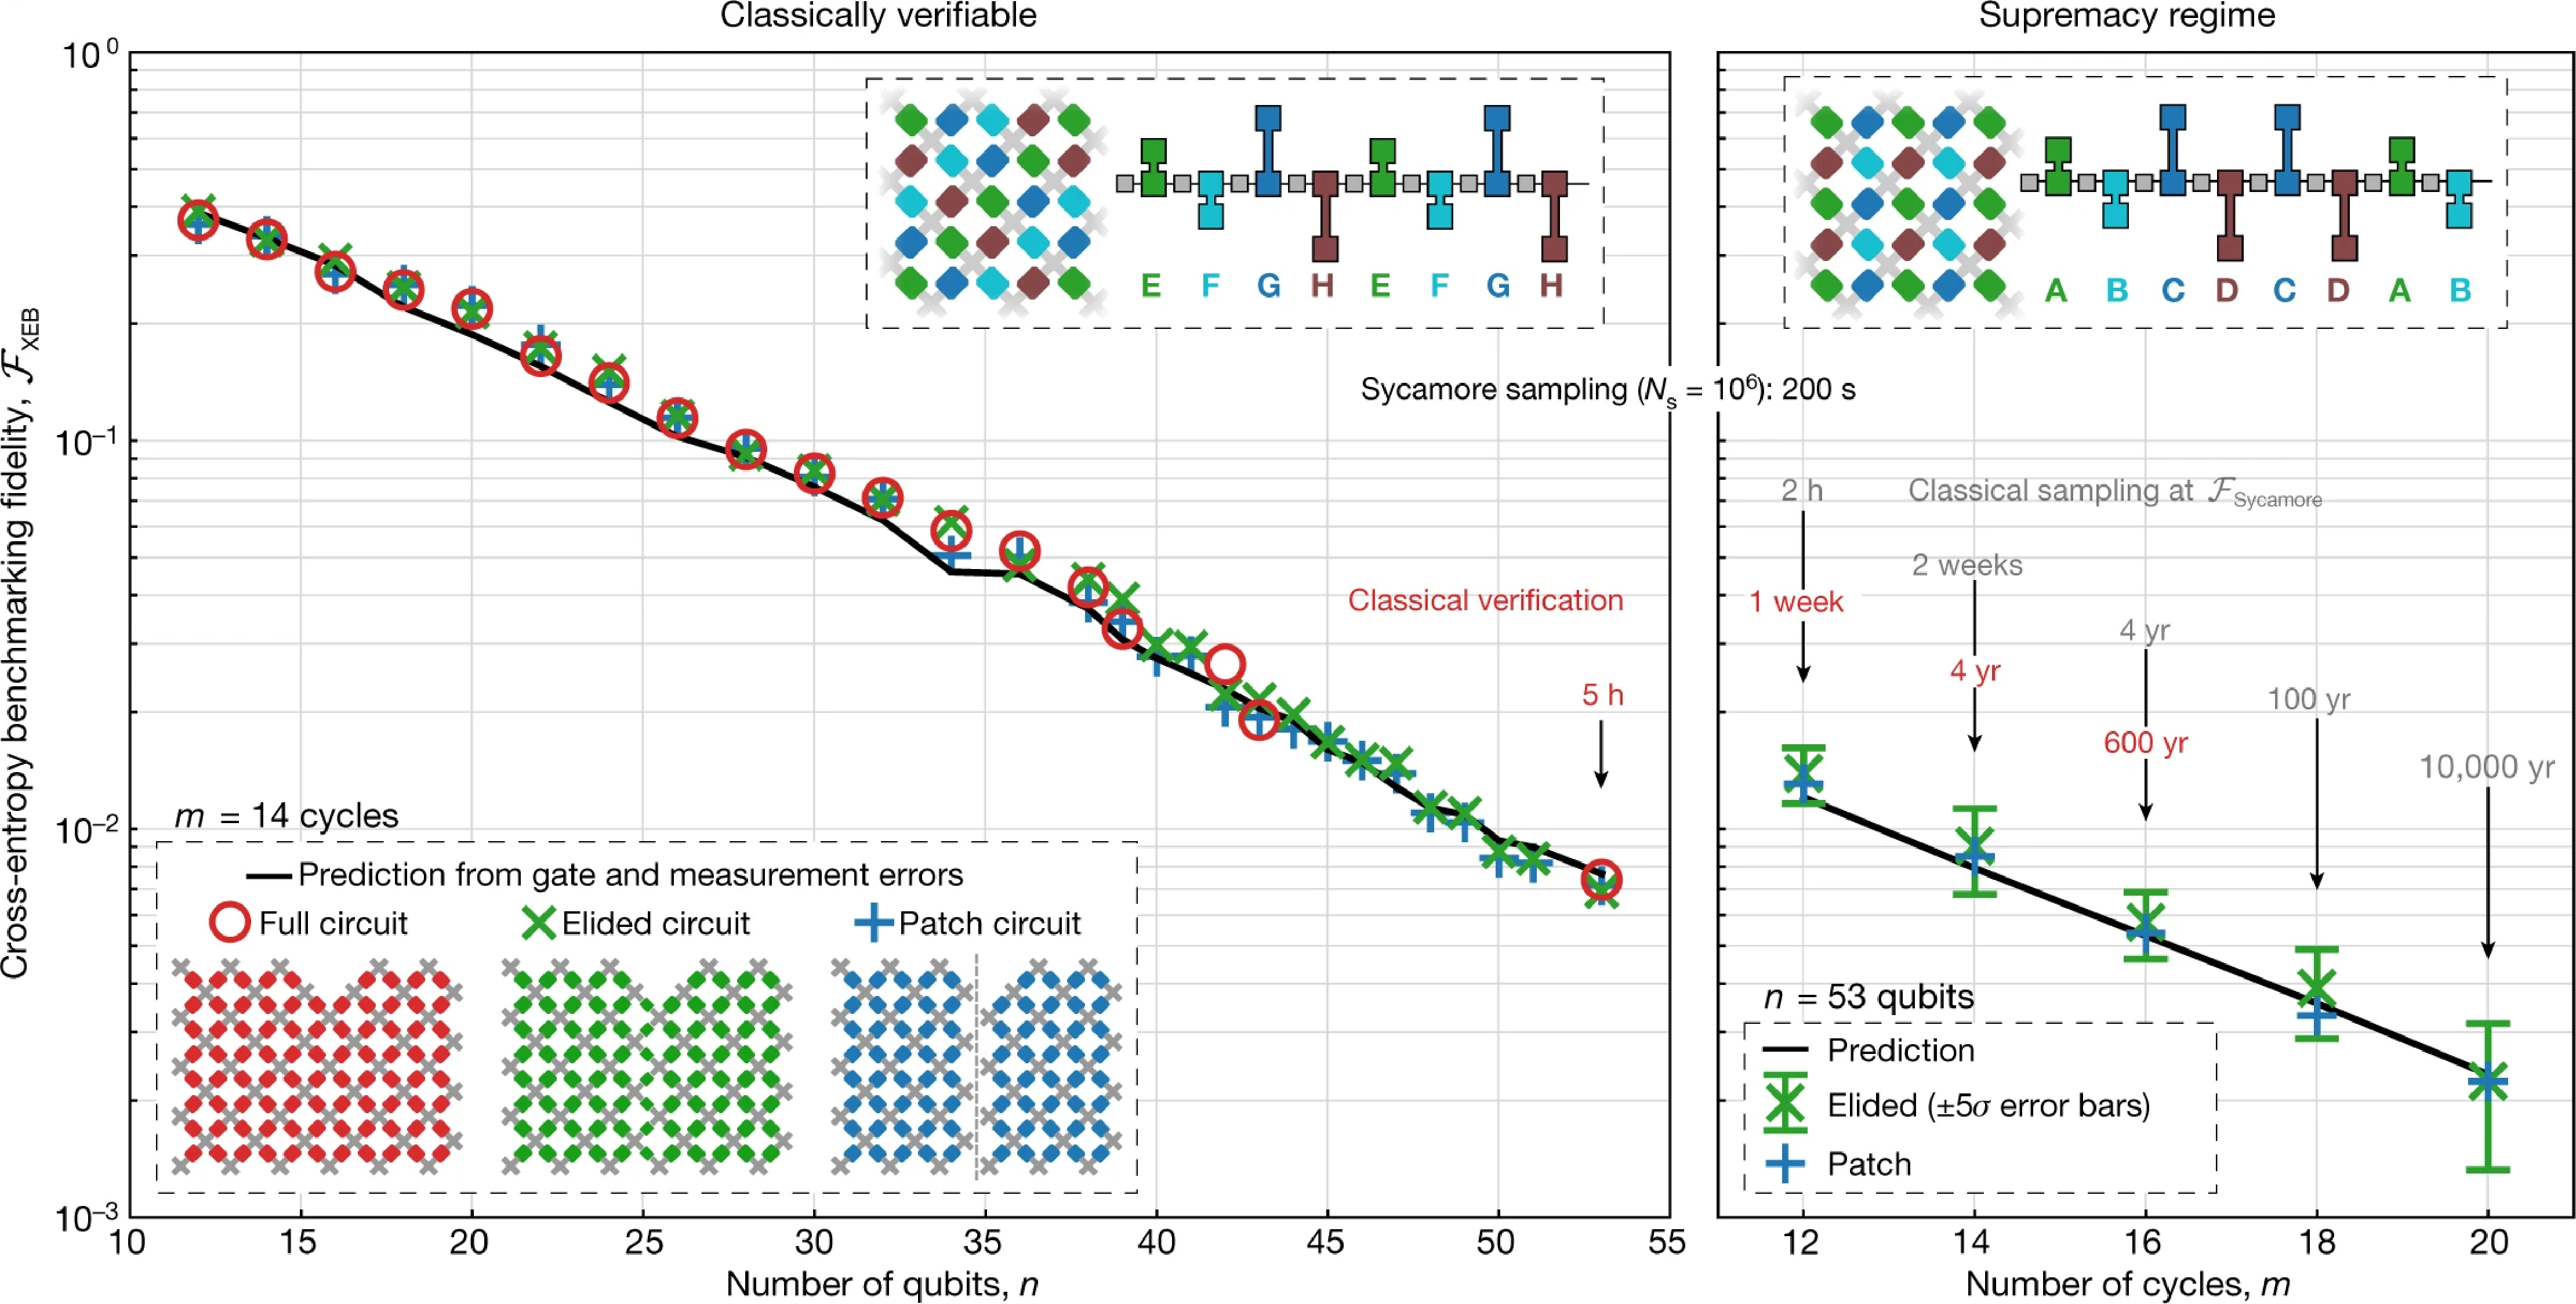
\includegraphics[width=\textwidth]{figures/supremacy_results}
  \caption[Cross Entropy Fidelity of the Sycamore Processor]{Results from the quantum supremacy experiments 
  with the Sycamore processor \cite{martines2019supremacy}. The full circuits could only be simulated up to $n=53$ qubits and 
  $m=12$ cycles. Experiments on elided and patched circuits match the values of the extrapolated cross entropy fidelity.}
\end{figure}

The team reports an average circuit fidelity $ > 0.1\%$ with $5\sigma$ confidence
for the largest elided circuits. All results fit the extrapolated expected
fidelity from smaller circuits, making the team conclude that similar fidelities
would be confirmed for the full circuits. As classical simulations of these
circuits would take up to 100,000 years according to the team with a hybrid
Schroedinger-Feynman algorithm, this would imply
that quantum supremacy has been achieved \cite{martines2019supremacy}. The reported fidelities of the quantum supremacy for
the different circuit sizes and depths are reported in figure~\ref{fig:supremacy_results}.

Shortly after these results have been announced, researchers from IBM claimed that the classical simulations
for the full circuits on 53 qubits and 20 cycles could have been performed
on the Summit supercomputer within a few days only with an optimized memory
usage \cite{pednault2019leveraging}. Experimental proof for these claims is still to be given.

Even if these circuits can be simulated within a few days, the quantum
processor would still outperform the classical simulation as it only
takes about 200ms to generate the 2 million samples for those circuits from it. As quantum
supremacy is a loosely defined term, the discussion might continue whether
quantum supremacy has been demonstrated by the Google and UCSB team. Nevertheless, 
the resuts proof that it is possible to build a quantum processor of 53 qubits
which can execute quantum circuits consisting of up to 1,113 single-qubit and
430 two-qubit gates. For the future, the Google team expects a double exponential growth of the computational
power of quantum computers as the classical simulation costs grow exponentially
with the computational volume (gates and qubits) and quantum hardware
improvements will probably follow a quantum processor equivalent of Moore's law \cite{martines2019supremacy}.

This study does not focus on quantum circuits running on physical quantum devices,
but rather on the classical simulation. New and improved classical
approximate simulations of quantum systems with neural networks recently proved
to work well on many problem instances. 
Understanding their performance and necessary computational resources on
the RCS task might provide useful insights about the capabilities and
limitations of neural networks for the classical simulation of quantum systems.
\chapter{Boltzmann Machines}
\label{sec:rbm}
The following chapter gives an introduction to Boltzmann machines and their applications to the classical 
simulation of quantum computing.

An overview of the architecture and mathematical properties of Boltzmann machines are given in the first section. The restricted Boltzmann machine is motivated as a special kind of Boltzmann machine with useful mathematical properties in the second part of this chapter. Afterward, the concepts of Gibbs sampling and supervised learning are explained.
In the last section, a constructive approach on how restricted Boltzmann machines 
can be applied to the classical simulation of quantum computing is given.

The introduction to Boltzmann machines and restricted Boltzmann machines as well as the introduction 
to Gibbs sampling are based on \cite{montufar2018restricted} and 
\cite{fischer2012introduction} which provide a more throughout introduction 
into the topic. The work of J\'{o}nsson, Bauer and Carleo \cite{jnsson2018neuralnetwork} is the 
foundation of the last section of this chapter.

\section{Characteristics}
\label{sec:gbm}
The concept of the Boltzmann machine has first been proposed in the 1980s as a
model for parallel distributed computing \cite{hinton1983analyzing}. Boltzmann machines are physically inspired by the Ising Spin model and can be interpreted as energy-based recurrent neural networks representing probability distributions
over vectors $\bm{d}_i \in \{0,1\}^n$ \cite{ackley1985learning}.

A Boltzmann machine is a network of stochastic units (or neurons) $X=V \cup H$ which are segmented into
\textit{visible} neurons $V=\{v_1, \dots, v_n\}$ and \textit{hidden} neurons $H=\{h_1, \dots, h_m\}$.
The joint state of the visible neurons $\bm{v} = (v_1\dots v_n) \in \{0,1\}^n$ represents n-dimensional data
points $\bm{d}_i \in \{0,1\}^n$. The hidden neurons increase the expressiveness of the Boltzmann machine by acting as non-linear feature 
detectors to model dependencies between the visible neurons \cite{hinton2010boltzmann}.

The neurons are 
connected to each other by weighted links $W_{ij}$ and poss biases $a_i$ (visible) or $b_i$ (hidden), respectively. In 
general, the neurons of a Boltzmann machine can be fully connected. A graphical representation of a fully connected Boltzmann machine is shown in figure~\ref{fig:boltzmannMachine}.

\begin{figure}[H]
    \centering
    \begin{tikzpicture}[transform shape,line width=0.2pt]
        \foreach \x in {1,...,8}{%
            \pgfmathparse{(\x-1)*45+floor(\x/9)*22.5}
            \node[label={\pgfmathresult:\ifnum\x=1 $v_5$\else\ifnum\x=2 $h_3$\else\ifnum\x=3 $h_2$\else\ifnum\x=4 $h_1$\else\ifnum\x=5 $v_1$\else\ifnum\x=6 $v_2$\else\ifnum\x=7 $v_3$\else\ifnum\x=8 $v_4$\fi\fi\fi\fi\fi\fi\fi\fi},draw,circle,inner sep=0.25cm,fill={\ifnum\x=1 yellow\else\ifnum\x<5 cyan\else yellow\fi\fi}] (N-\x) at (\pgfmathresult:2.8cm) [thick] {\ifnum\x=1 $a_5$\else\ifnum\x=2 $b_3$\else\ifnum\x=3 $b_2$\else\ifnum\x=4 $b_1$\else\ifnum\x=5 $a_1$\else\ifnum\x=6 $a_2$\else\ifnum\x=7 $a_3$\else\ifnum\x=8 $a_4$\fi\fi\fi\fi\fi\fi\fi\fi};
        }
        \foreach \x [count=\xi from 1] in {2,...,8}{%
            \foreach \y in {\x,...,8}{%
                \ifnum\y=5 \else\ifnum\xi=5 \else \path (N-\xi) edge[-] (N-\y)\fi\fi;
            }
        }
        \draw (N-5) -- (N-1) node [] (E-1) {};
        \draw (N-5) -- (N-2) node [] (E-2) {};
        \draw (N-5) -- (N-3) node [] (E-3) {};
        \draw (N-5) -- (N-4) node [midway,above=-0.06cm,sloped] (E-4) {$W_{v_{1}h_{1}}$};
        \draw (N-5) -- (N-6) node [] (E-5) {}; 
        \draw (N-5) -- (N-7) node [] (E-6) {};
        \draw (N-5) -- (N-8) node [] (E-7) {};
    \end{tikzpicture}
    \caption[Fully Connected Boltzmann Machine]{Graphical representation of a fully connected Boltzmann machine with 5 visible neurons (yellow) $v_1$ to $v_5$
    and 3 hidden neurons (blue) $h_1$ to $h_3$. Each neuron posses a bias
    $a_1$ to $a_5$ and $b_1$ to $b_3$ respectively. The connection weight between two neurons $i$ and $j$
    is given by $W_{ij}$.}
    \label{fig:boltzmannMachine}
\end{figure}

Each configuration $\bm{c}=(v_1,\dots,v_n,h_1,\dots,h_m)$ of neuron states
of the Boltzmann machine is associated with an energy $E(\bm{c})$ value,
which is defined by the parameters $\mathcal{W}$ consisting of the weights and 
biases $\mathcal{W} = \{a_i, b_j, W_{ij}\}$:

\begin{equation}
  E(\bm{c};\mathcal{W}) = - \sum_{v_i \in V} a_{i}v_{i} - \sum_{h_i \in H} b_{i}h_{i} - \sum_{x_i,x_j \in X} W_{x_i,x_j}x_{i}x_{j}.
\end{equation}

When sampling configurations from the Boltzmann machine (discussed in more detail in section~\ref{sec:gibbsSampling}), the 
Boltzmann machine prefers low energy states over states with high energies. The \textit{stationary probability}
of a configuration $\bm{c}$ with energy $E(\bm{c};\mathcal{W})$ is given by the so-called \textit{Gibbs-Boltzmann distribution} \cite{gibbs_2010}

\begin{equation}
   p(\bm{c};\mathcal{W}) = \frac{\mathrm{e}^{-E(\bm{c};\mathcal{W})}}{Z(\mathcal{W})},
\end{equation}

where $Z(\mathcal{W})$ is the normalizing partition function 

\begin{equation}
   Z(\mathcal{W}) = \sum_{\bm{c}\prime\in C} \mathrm{e}^{-E(\bm{c}\prime;\mathcal{W})}.
\end{equation}

In a training phase (discussed in section~\ref{sec:learning} ), the parameters of the Boltzmann machine can be adapted in such a way that 
the marginal probability distribution $p(\bm{v}; \mathcal{W})$ of the visible neurons

\begin{equation}
    \label{eq:gbm}
   p(\bm{v};\mathcal{W}) = \sum_{\bm{h}_k \in \{0,1\}^m} p(\bm{v},\bm{h}_k;\mathcal{W}),
\end{equation}

which traces out the hidden unit 
states by summing over all possible configurations of them, resembles the probability 
distribution of data points $\bm{d}_i$ in a training set $D=\{\bm{d}_1,\dots,\bm{d}_l\}$.

For a fully connected Boltzmann machine, this representation consists of an exponential number of summands and cannot be calculated efficiently. So-called \textit{restricted Boltzmann machines}
have a specific architecture with a restricted connectivity, which allows the efficient calculation of the marginal probability.

\section{Restricted Boltzmann Machines}
\label{sec:rbms}
The \gls{rbm} is a type of Boltzmann machine with 
a specific architecture and properties \cite{smolensky1986information}. Since their invention \gls{rbm}s have been applied to a variety 
of machine learning tasks. They played a 
key role in the development of deep learning architectures as building blocks of so-called 
\textit{Deep Belief networks} \cite{bengio2009learning, hinton2006fast}.
\gls{rbm}s are the kind of Boltzmann machines which are used in this study of the simulation 
of quantum circuits.

In its restricted form, the neurons of the Boltzmann machine are separated into two layers;
one being the visible layer containing the visible neurons $v_i \in V$ and the other layer being the hidden layer containing the hidden neurons $h_j \in H$. Each neuron of the \gls{rbm} 
is only allowed to be connected to the neurons from the other layer. Intra-layer connections are not allowed. As a result, the graph of the \gls{rbm} is bipartite as shown in figure~\ref{fig:rbm}. 

\begin{figure}[H]
    \centering
    \begin{tikzpicture}[transform shape,line width=0.2pt]
    
        \node (v1)[neuron, fill=yellow] at (0, 0) {$a_1$};
        \node (v2)[neuron, fill=yellow] at (2, 0) {$a_2$};
        \node (v3)[neuron, fill=yellow] at (4, 0) {$a_3$};
        \node (v4)[neuron, fill=yellow] at (6, 0) {$a_4$};
        \node[below=0.1cm of v1] (bv1) {$v_1$};
        \node[below=0.1cm of v2] (bv2) {$v_2$};
        \node[below=0.1cm of v3] (bv3) {$v_3$};
        \node[below=0.1cm of v4] (bv4) {$v_4$};
    
        \node (h1)[neuron, fill=cyan] at (1, 2) {$b_1$};
        \node (h2)[neuron, fill=cyan] at (3, 2) {$b_2$};
        \node (h3)[neuron, fill=cyan] at (5, 2) {$b_3$};
        \node[above=0.1cm of h1] (bh1) {$h_1$};
        \node[above=0.1cm of h2] (bh2) {$h_2$};
        \node[above=0.1cm of h3] (bh3) {$h_3$};
    
        \draw (v1) -- (h1) node [midway,above=-0.06cm,sloped] {$W_{v_1h_1}$};
        \draw (v1) -- (h2) node [midway,above=-0.06cm,sloped] {};
        \draw (v1) -- (h3) node [midway,above=-0.06cm,sloped] {};
    
        \draw (v2) -- (h1) node [midway,above=-0.06cm,sloped] {};
        \draw (v2) -- (h2) node [midway,above=-0.06cm,sloped] {};
        \draw (v2) -- (h3) node [midway,above=-0.06cm,sloped] {};
    
        \draw (v3) -- (h1) node [midway,above=-0.06cm,sloped] {};
        \draw (v3) -- (h2) node [midway,above=-0.06cm,sloped] {};
        \draw (v3) -- (h3) node [midway,above=-0.06cm,sloped] {};
    
        \draw (v4) -- (h1) node [midway,above=-0.06cm,sloped] {};
        \draw (v4) -- (h2) node [midway,above=-0.06cm,sloped] {};
        \draw (v4) -- (h3) node [midway,above=-0.06cm,sloped] {};
    \end{tikzpicture}
    \caption[Restricted Boltzmann Machine]{Graphical representation of a \gls{rbm} with 5 visible neurons and 3 hidden ones. 
    There are only connections between the two layers and no connection between two neurons 
    from the same layer.}
    \label{fig:rbm}
\end{figure}

The marginal probability $p(\bm{v};\mathcal{W})$ of the visible neuron states in a \gls{rbm} has the form:

\begin{align}
   p(\bm{v};\mathcal{W}) &= \sum_{\bm{h}_k \in \{0,1\}^m} p(\bm{v},\bm{h}_k;\mathcal{W})\\
   &= \frac{1}{Z(\mathcal{W})}\sum_{\bm{h}_k \in \{0,1\}^m} \mathrm{e}^{-E(\bm{v}, \bm{h}_k;\mathcal{W})}\\
   &= \frac{1}{Z(\mathcal{W})}\sum_{h_1\in \{0,1\}}\dots\sum_{h_m \in \{0,1\}}\mathrm{e}^{\sum_{v_i}b_iv_i}\prod_{j=1}^m\mathrm{e}^{h_j(b_j + \sum_{i=1}^nW_{ij}v_i)}\\
   &= \frac{\mathrm{e}^{\sum_{v_i}b_iv_i}}{Z(\mathcal{W})}\sum_{h_1 \in \{0,1\}}\mathrm{e}^{h_1(b_1 + \sum_{i=1}^nW_{i1}v_i)}\dots\sum_{h_m \in \{0,1\}}\mathrm{e}^{h_m(b_m + \sum_{i=1}^nW_{im}v_i)}\\
   &= \frac{\mathrm{e}^{\sum_{v_i}b_iv_i}}{Z(\mathcal{W})}\prod_{i=1}^m\sum_{h_i \in \{0,1\}}\mathrm{e}^{h_i(b_i + \sum_{i=1}^nW_{ij}v_i)}\\
   \label{eq:rbm}
   &= \frac{\mathrm{e}^{\sum_{v_i}b_iv_i}}{Z(\mathcal{W})}\prod_{i=1}^m(1+\mathrm{e}^{b_i + \sum_{i=1}^nW_{ij}v_i}).
\end{align}

This quantity consists of only a polynomial number of terms in the number of hidden units of the \gls{rbm}. Consequently, it can be calculated efficiently. This makes the \gls{rbm} a compact representation of a probability distribution over vectors $\bm{d}_i \in D$ inferred from a dataset $D$.

Even though the \gls{rbm} has a limited connectivity between its units, it is a universal function approximator \cite{le2008representational}.
It can model any distribution over $\{0,1\}^m$ arbitrary well with $m$ visible and $k+1$ hidden units, where 
$k$ denotes the cardinality of the support set of the target distribution. This is the number of input elements
from $\{0,1\}^m$ that have a non-zero probability of being observed. This also implies a worst-case 
exponential number of hidden units for distributions with an extensive support set \cite{le2008representational}. Fewer units can be sufficient depending on the patterns in the support set \cite{montufar2011refinements}.

\section{Gibbs Sampling}
\label{sec:gibbsSampling}

Boltzmann machines are generative models that represent probability distributions over their configurations. This means that it is possible to draw configurations from a Boltzmann machine
according to their (marginal) probabilities given in equations~\ref{eq:gbm} and \ref{eq:rbm}.

Although it is required to calculate $Z(\mathcal{W})$ for the exact probabilities of each configuration,
it is not necessary to calculate the energies for all $2^{n+m}$ possible configurations of 
a Boltzmann machine to draw samples from it.

Instead, Boltzmann machines can be seen as \textit{Markov chains} with a stationary probability
distribution. With a stochastic process called \textit{Gibbs sampling} the samples can be drawn efficiently according to this stationary distribution for \gls{rbm}s.

Gibbs sampling belongs to the class of so-called \textit{Metropolis-Hastings} algorithms. By that, it is 
a \textit{\gls{mcmc}} algorithm \cite{hastings1970monte}. It is a simple algorithm to produce samples from the joint probability distribution of multiple random variables like neuron state configurations
of a Boltzmann machine, which can be considered as a Markov chain.

A Markov chain is a discrete stochastic process of configurations of random variables $C=\{\bm{c}^{(t)}\}$
at time steps $t=1, \dots, T$ which take values in a set $\Omega$ (for Boltzmann machines 
$\Omega=\{0,1\}^{m+n}$) and for which for all time steps $t$ and for all configurations 
$\bm{c}_j, \bm{c}_i, \bm{c}_{i-1}, \dots, \bm{c}_0 \in \Omega$ the \textit{Markov property}

\begin{align}
    p_{ij}^{(t)} &:= P(\bm{c}^{(t+1)} = \bm{c}_j \mid \bm{c}^{(t)} = \bm{c}_i, \dots, \bm{c}^{(0)} = \bm{c}_0) \\
                 & = P(\bm{c}^{(t+1)} = \bm{c}_j \mid \bm{c}^{(t)} = \bm{c}_i) 
\end{align}

holds. This means that the next state of the system only depends on the current state and not on the system's history. A Markov chain can be represented as a (finite) graph, as shown in figure~\ref{fig:markov}.

\begin{figure}[H]
    \centering
    \begin{tikzpicture}[transform shape,line width=0.2pt]
    
        \node [draw,circle,inner sep=0.25cm] (s0) at (0,0) {$c_0$};
        \node [draw,circle,inner sep=0.25cm] (s1) at (3,0) {$c_1$};
    
        \path[->] (s0) edge[loop left]  node {$p_{00}$} (s0);
        \path[->] (s0) edge[bend left] node[above] {$p_{01}$} (s1);
        \path[->] (s1) edge[bend left] node[below] {$p_{10}$} (s0);
        \path[->] (s1) edge[loop right] node {$p_{11}$} (s1);
    
    \end{tikzpicture}
    \caption[Markov Chain with Two States]{A Markov chain with two states $c_0$ and $c_1$. The Markov chain is 
described by the $2 \times 2$ matrix $\bm{P}=\begin{pmatrix} p_{00} & p_{01} \\ p_{10} & p_{11} \end{pmatrix}$.}
    \label{fig:markov}
\end{figure}

In the case of Boltzmann machines, the transition probabilities $p_{ij}$ are time independent and 
given by the ratios of configuration probabilities. For \gls{rbm}s the transition probability $p_{ij}$ 
from configuration $c_i$ to $c_j$ is given by:

\begin{equation}
    p_{ij} = \frac{\mathrm{e}^{\sum_{v_i \in \bm{c_i}}b_iv_i}\prod_{i=1}^m(1+\mathrm{e}^{b_i + \sum_{i=1}^nW_{ij}v_i})}{\mathrm{e}^{\sum_{v_i \in \bm{c_j}}b_iv_i}\prod_{i=1}^m(1+\mathrm{e}^{b_i + \sum_{i=1}^nW_{ij}v_i})},
\end{equation}

which can be calculated efficiently as the $Z(\mathcal{W})$ terms from equation~\ref{eq:rbm} cancel out.

In each time step $t$ during the Gibbs sampling, the state of a single randomly chosen neuron of the \gls{rbm} is flipped
so that the configurations $\bm{c}^{(t)}$ and $\bm{c}^{(t+1)}$ only differ in the state of one neuron. With 
probability $p_{ij}$ configuration $\bm{c}_j$ is kept as the new configuration. With probability
$1-p_{ij}$ the Boltzmann machine will stay in its current configuration $\bm{c}_i$. This corresponds to a random walk on the Markov chain defined by the \gls{rbm} transition probabilities. The algorithm is given in 
algorithm~\ref{alg:gibbs}.

\begin{algorithm}[H]
    \caption{Gibbs Sampling}
    \begin{algorithmic}[1]
        \Require $bm(\bm{c})$: function returning the energy of a Boltzmann machine for configuration $\bm{c}$
        \Require T: time steps
        \State $t\gets 0$
        \State $\bm{c}^{(0)} \gets randomize(\{0,1\}^{m+n})$ (random initialization)
        \Repeat
            \State $r \gets random(m+n)$
            \State $E_i \gets bm(\bm{c}^{(t)})$
            \State $E_j \gets bm(\{c_1,\dots,\bar{c_r},\dots,c_{m+n}\})$
            \If{$random(1) < \frac{E_i}{E_j}$}
                \State $\bm{c}^{(t+1)} \gets \{c_1,\dots,\bar{c_r},\dots,c_{m+n}\}$
            \EndIf
            \State $t\gets t+1$
        \Until{$t=T$}
        \State \textbf{return} $\bm{c}^{(T)}$
    \end{algorithmic}
    \label{alg:gibbs}
\end{algorithm}

The Markov chain for configurations of a Boltzmann machine is known to converge to its so-called 
\textit{stationary distribution} $\pi$, that is

\begin{equation}
    \pi^T=\pi^T\bm{P}
\end{equation}

with $\bm{P} = (p_{ij})$ being the transition matrix of the Markov chain with the transition probabilities as its entries.
Once the Markov chain reaches its stationary distribution, all subsequent states will be distributed according to this distribution. Running Gibbs sampling for 
sufficiently many time steps $T$ will sample configurations according 
to the Gibbs-Boltzmann distribution given in equation~\ref{eq:rbm}.

Although Gibbs sampling is a simple algorithm, it is an important algorithm in the context of 
Boltzmann machines. Different versions of Gibbs sampling have been developed for \gls{rbm}s, like 
(persistent) contrastive divergence \cite{hinton2002training, tieleman2008training} or parallel tempering \cite{desjardins2010parallel}. In this study,
Gibbs sampling is used in its simplest version, as described in this chapter.
    
\section{Supervised Learning}
\label{sec:learning}
The probability distribution over vector spaces given by a Boltzmann machine can be trained to 
resemble the distribution of data points $\bm{d}_i$ in a dataset $D=\{\bm{d}_1,\dots,\bm{d}_d\}$. This can be done either in a \textit{unsupervised}
or in a \textit{supervised} manner.

In both cases the parameters $\mathcal{W} = \{a_i,b_j,W_{ij}\}$ of the Boltzmann machine are updated minimizing 
an objective function $O(\mathcal{W})$, which depends on the parameters of the Boltzmann machine and 
depicts the overlap of the current and the target distribution in an iterative process called \textit{gradient descent}.

Before the training phase, the Boltzmann machine is initialized with random parameters $\theta_i \in \mathcal{W}_0$ and a training set 
$D=\{\bm{d}_1,\dots,\bm{d}_d\}$ is given. In the case of supervised learning of Boltzmann machines, the training set consists of tuples of configurations and their corresponding target energy values $\bm{d}_i= (\bm{c}_i, t_i)$.

In the batch version of gradient descent the training set $D$ is 
split into subsets $D_1, \dots, D_l$, called \textit{batches}.

For each such batch $D_i$ the average negative log overlap $\langle L(\mathcal{W})\rangle$ for all $\bm{c}_j \in D_i$
is computed. Afterward, the gradients $\frac{\partial L}{\partial \delta_i}$ are calculated and the parameters updated into
the direction of the steepest descent:

\begin{equation}
    \label{eq:sgd}
    \theta_i = \theta_i - \alpha \frac{\partial L}{\partial \delta_i}
\end{equation}

with \textit{learning rate} $\alpha \ll 1$ to keep the step sizes moderate. The learning rate prevents step sizes, which are too big in steep 
areas of the objective function $L(\mathcal{W})$.
This process is repeated for a defined number of iterations to minimize the objective function $O(\mathcal{W})$.
A graphical representation of this process is shown in figure~\ref{fig:sgd}.

\begin{figure}[H]
  \centering
  \includegraphics[width=0.8\textwidth]{figures/gradient_descent}
  \caption[Gradient Descent]{Iterations of a gradient descent method. At each iteration the randomly initialized parameters are updated in 
   direction of the steepest descent of the function to be optimized. After enough iterations a minimum of the function is reached.}
  \label{fig:sgd} 
\end{figure}
 
The simple update rule in \ref{eq:sgd} has several drawbacks, however. First, The gradient and the step size become smaller as closer the function approaches its minimum, leading to only small improvements and many steps necessary.
Second, the function's shape will usually have (many) local minima, which should be avoided.
Several variants of gradient descent have been developed to overcome these issues \cite{ruder2016overview}.
Two of these methods are \textit{AdaMax} \cite{ruder2016overview} and \textit{\gls{sr}} \cite{sorella1998green}.

\subsection{AdaMax}
AdaMax is a special version 
of \textit{Adam} \cite{kingma2014adam}.It combines the advantages of AdaGrad \cite{duchi2011adaptive} and RMSProp \cite{bengio2015rmsprop},
two other popular gradient descent methods. AdaMax is computationally efficient, has little
memory requirements, and proves to be well suited for problems with much noise and sparse gradients.

Instead of using the raw gradient, the algorithm updates exponential moving averages of the gradient ($\bm{m}_t$) and the squared gradient
($\bm{v}_t$) to include more information about the shape of the error function into the parameter updates. The hyper-parameters $\beta_1, \beta_2 \in [0, 1)$ control the exponential decay rates of these moving
averages. The moving averages themselves are estimates of the 1st moment (the mean) and the
2nd raw moment of the gradient. The update rule for the parameters $\theta_{i} \in \mathcal{W}$ for AdaMax are summarized in 
algorithm~\ref{alg:adamax}.

\begin{algorithm}
    \caption{AdaMax}
    \begin{algorithmic}[1]
        \Require $\alpha$: step size
        \Require $\beta_1, \beta_2 \in [0,1)$: Exponential decay rates
        \Require $f(\mathcal{W})$: Stochastic objective function
        \Require $\mathcal{W}_0$: Initial parameter vector
        \State $\bm{m}_0 \gets \bm{0}$ (Initialize $1^{st}$ moment vector)
        \State $\bm{u}_0 \gets \bm{0}$ (Initialize the exponential weighted infinity norm)
        \State $t \gets 0$ (Initialize time step)
        \While {$\mathcal{W}_t$ not converged}
            \State $t\gets t+1$
            \State $\bm{g}_t \gets \nabla_{\mathcal{W}}f_t(\mathcal{W}_{t-1})$ (Get gradients w.r.t. objective function at time step $t$)
            \State $\bm{m}_t \gets \beta_1 \cdot m_{t-1} + (1-\beta_1) \cdot \bm{g}_t$ (Update biased first moment estimate)
            \State $\bm{u}_t \gets max(\beta_2 \cdot u_{t-1}, \vert{\bm{g}_t})$ (Update the exponentially weighted infinity norm)
            \State $\mathcal{W}_t \gets \mathcal{W}_{t-1} - (\alpha/ (1-\beta_1^t)) \cdot \bm{m}_t/\bm{u}_t$ (Update parameters)
        \EndWhile
        \State \textbf{return} $\mathcal{W}_t$ (Resulting parameters)
    \end{algorithmic}
    \label{alg:adamax}
\end{algorithm}

\subsection{Stochastic Reconfiguration}
Another popular gradient descent method to optimize the parameters of an \gls{rbm} to represent quantum states is 
\textit{Stochastic reconfiguration} \cite{sorella1998green}. The idea behind this method is that even a small change in the 
parameters of the \gls{rbm} might lead to a big change in the output distribution of the \gls{rbm}. Instead of small steps
 in the parameter space as in the pure version of gradient descent, the step size is kept small 
with respect to the change in the output distribution represented by the \gls{rbm}. Stochastic reconfiguration is equivalent 
to the \textit{natural gradient descent} method \cite{amari1998natural}.

The update rule for the parameters $W$ of the \gls{rbm} in the \gls{sr} method is:

\begin{equation}
    \theta_i^{\prime} = \theta_i - \alpha \bm{S}^{-1} \bm{f}
\end{equation}

with

\begin{align}
    \bm{f}_i &= \langle \Delta_i^* \frac{\partial O}{\partial \theta_i} \rangle - \langle \Delta_i^* \rangle \langle \frac{\partial O}{\partial \theta_i} \rangle \\
    \bm{S}_{ij} &= \langle \Delta_i^* \Delta_j \rangle - \langle \Delta_i^* \rangle \langle \Delta_j \rangle
\end{align}

where $\langle x \rangle$ denotes the mean of a random variable $x$ and $\Delta_i$ denotes the log-derivative of 
of the wave function $\Delta_i(\bm{c}) = \frac{1}{\psi(\bm{v})}\frac{\partial \psi(\bm{c})}{\partial \theta_i}$ with 
respect to some paramter $\theta_i \in \mathcal{W}$.

Using the covariance matrix $\bm{S}$ of the derivatives of the wave function keeps the KL-divergence between 
the \gls{rbm} before and after the update low, leading to a smooth transition through the error landscape \cite{sorella1998green}.

Both AdaMax and Stochastic reconfiguration are modifications to the standard gradient descent method which 
try to reduce oscillations during the training and time to convergence by including more information about the 
shape of the error function into the changes of the gradients. This study compares both methods for the classical simulation of quantum computing with \gls{rbm}s.

\section{Application to Quantum Computing}
\label{sec:applicationToQuantumComputing}
Machine learning techniques have become a successful approach for the classical simulation
of quantum systems \cite{carleo2017solving, deng2017quantum, carleo2018constructing}. 
Carleo and Troyer \cite{carleo2017solving} were the first to give a compact presentation of the wave function of a many-body quantum system with an \gls{rbm}.
The same framework has later been used by J\'{o}nsson, Bauer, and Carleo for the classical simulation of the quantum Fourier and Hadamard transform \cite{jnsson2018neuralnetwork}. Their work gives a constructive approach on how the parameters of a complex-valued \gls{rbm} representing the quantum state

\begin{equation}
   \Ket{\psi_{\mathcal{W}}(\bm{v})} = \frac{\mathrm{e}^{\sum_{v_i}b_iv_i}}{Z(\mathcal{W})}\prod_{i=1}^m(1+\mathrm{e}^{b_i + \sum_{i=1}^nW_{ij}v_i})
\end{equation}

can be adapted to apply a universal set of quantum gates to the quantum state $\Ket{\psi_{\mathcal{W}}}$.

\gls{rbm}s allow an exact application of unitary gates diagonal in the computational basis. For non-diagonal 
gates more hidden layers would be necessary, making the calculation of the quantum state intractable \cite{carleo2018constructing}. Nevertheless, it is possible to train a Boltzmann machine in a supervised fashion, such that its parameters are adapted to apply a non-diagonal gate to its state approximately.

The rules for the applications of diagonal and non-diagonal gates to an \gls{rbm} state from 
\cite{jnsson2018neuralnetwork} are laid out in following two sections.

\subsection{Diagonal Gates}

Diagonal gates can be applied to an \gls{rbm} quantum state by solving a set of linear equations. 
This section describes the rules for the applications of single-qubit $Z$ rotations, controlled $Z$ rotations 
as well as the Pauli $X$, $Y$ and $Z$ gates.

\subsubsection{Single-Qubit $Z$ rotations}
The action of the single $Z$ rotation of angle $\theta$ is given by the $2\times2$ unitary matrix

\begin{equation}
    R_l^Z=
    \begin{pmatrix}
        1 & 0 \\
        0 & \mathrm{e}^{i\theta}
    \end{pmatrix} .
\end{equation}

Its action on qubit $l$ yields 
$\langle \bm{v} \mid R_{l}^{Z}(\theta) \mid \psi_{W}  \rangle = 
\mathrm{e}^{i\theta v_{l}} \Ket{\psi_{W}(\bm{v})}
$
. Considering a \gls{rbm} machine with weights $\mathcal{W}^{\prime} = \{\alpha^{\prime},\beta^{\prime},W^{\prime}\}$, the action of the $R^{Z}(\theta)$
gate is exactly reproduced if $\mathrm{e}^{v_{l}a_{l}}\mathrm{e}^{i\theta v_{l}} = \mathrm{e}^{v_{l}a\prime_{l}}$
is satisfied. This is the case for

\begin{equation}
    a^{\prime}_{j} = a_{j} + \delta_{jl}i\theta.
\end{equation}

The action of the Z rotation modifies the bias of the visible neuron $l$ of the \gls{rbm}.

\subsubsection{Controlled Z rotations}
The action of a controlled Z rotations acting on two given qubits $l$ and $m$ is determined by
the $4\times4$ unitary matrix

\begin{equation}
    CZ =
    \begin{pmatrix}
        1 & 0 & 0 & 0 \\
        0 & 1 & 0 & 0 \\
        0 & 0 & 1 & 0 \\
        0 & 0 & 0 & \mathrm{e}^{i\theta}
    \end{pmatrix},
\end{equation}

where $\theta$ is a given rotation angle. This gate is diagonal and can compactly be written as

\begin{equation}
    \langle \bm{v} \mid CZ(\theta) \mid \psi_{W}  \rangle = 
    \mathrm{e}^{i\theta v_{l}v_{m}}\Ket{\psi_{W}(v_{1} \dots v_{n})}.
\end{equation}

As the \gls{rbm} architecture does not allow direct interaction between visible neurons, the CZ gate
requires the insertion of a dedicated extra hidden unit $h_{c}$, which is connected
to the qubits $l$ and $m$

\begin{align}
    \langle \bm{v} \mid CZ(\theta) \mid \psi_{W}  \rangle &= 
    \mathrm{e}^{\Delta a_{l} B_{l} + \Delta a_{m} Z_{m}} \sum_{h_{c}}\mathrm{e}^{W_{lc} B_{l} h_{c} + W_{mc} B_{m} h_{c}} \\
    &= \mathrm{e}^{\Delta a_{l} B_{l} + \Delta a_{m} B_{m}} \times (1 + \mathrm{e}^{W_{lc} B_{l} + W_{mc}} B_{m}) \Ket{\psi_{W}(\bm{v})},
\end{align}

where the new weights $W_{lc}$ and $W_{mc}$ and visible units' biases $a_{l}\prime= a_{l} + \Delta a_{l}$,
$a_{m}\prime= a_{m} + \Delta a_{m}$ are determined by the equation

\begin{equation}
   \mathrm{e}^{\Delta a_{l} B_{l} + \Delta a_{m} B_{m}}(1 + \mathrm{e}^{W_{lc} B_{l} + W_{mc} B_{m}}) = C \times \mathrm{e}^{i \theta B_{l} B_{m}}
\end{equation}

for all the four possible values of the qubits states $B_{l}, B_{m} = \{0,1\}$ and where $C$ is an arbitrary (finite)
normalization. A possible solution for this system is

\begin{equation}
   W_{lc} = -2\mathrm{A}(\theta) 
\end{equation}

\begin{equation}
   W_{mc} = 2\mathrm{A}(\theta) 
\end{equation}

\begin{equation}
   \Delta a_{l} = i \frac{\theta}{2} + \mathrm{A}(\theta)
\end{equation}

\begin{equation}
   \Delta a_{m} = i \frac{\theta}{2} - \mathrm{A}(\theta)
\end{equation}

where $\mathrm{A}(\theta) = arccosh(\mathrm{e}^{-i \frac{\theta}{2}})$. Modifying the \gls{rbm}'s parameters 
accordingly applies a $CZ$ gate to its current state.

\subsubsection{Pauli X gate}
The X gate just flips the qubit $l$ and the \gls{rbm} amplitudes are

\begin{equation}
    \langle \bm{v} \mid X_{l} \mid \psi_{W}  \rangle = 
    \langle v_{1} \dots \bar{v_{l}} \dots v_{N} \mid \psi_{W} \rangle.
\end{equation}

Since $\bar{v_{l}} = (1-v_{l})$, it must be satisfied that

\begin{equation}
    (1-v_{l})W_{lk} + b_{k} = v_{l} W_{lk}\prime + b_{k}\prime
\end{equation}

and

\begin{equation}
   (1-B_{l}) a_{l} = B_{l} a_{l}\prime + C 
\end{equation}

hold for all the (two) possible values of $B_{l} = \{0,1\}$. The solution to these equations is

\begin{equation}
   W_{lk}\prime = -W_{lk}
\end{equation}

\begin{equation}
   b_{k}\prime = b_{k} + W_{lk}
\end{equation}

\begin{equation}
   a_{l}\prime = -a_{l}
\end{equation}

\begin{equation}
   C = a_{l},
\end{equation}

whereas all the $a_{j}$ and the other weights $W_{jk}$ with $j \neq i$ are unchanged.

\subsubsection{Pauli Y gate}
A similar solution is found for the $Y$ gate with the noticeable addition of extra phases
with respect to the $X$ gate

\begin{equation}
   W_{lk}\prime = -W_{lk}
\end{equation}

\begin{equation}
   b_{k}\prime = b_{k} + W_{lk}
\end{equation}

\begin{equation}
   a_{l}\prime = -a_{l} + i \pi
\end{equation}

\begin{equation}
   C = a_{l} + \frac{i \pi}{2},
\end{equation}

whereas all the $a_{j}$ and other weights $W_{jk}$ with $j \neq l$ are unchanged.

\subsubsection{Pauli Z gate}
The Pauli Z gate is a special case of the Z rotation with $\theta = \pi$. Thus the 
only necessary change is to set the bias $a_l$ of the visible neuron $l$ to

\begin{equation}
    a_{l}\prime = a_{l} + i \pi.
\end{equation}

\subsection{Non-Diagonal Gates}

Exact applications of non-diagonal gates to Boltzmann machine quantum states would require introducing a second hidden layer \cite{carleo2018constructing}. In contrast to an \gls{rbm} with just one hidden layer, this would make the calculation of the represented quantum state inefficient.

Thus, there are no rules for applying non-diagonal gates to an \gls{rbm} state similar to those for diagonal gates. Nevertheless, the parameters of the \gls{rbm} can be adapted in a 
supervised learning process instead.

The training set consists of samples drawn from the \gls{rbm} with its current set of parameters. In the sampling process, the \gls{rbm}'s energy function can be adapted to resemble the energy states after a non-diagonal unitary gate $ G $ has been applied to its state.

For any non-diagonal unitary gate

\begin{equation}
    G =  \begin{pmatrix}
        a & b \\
        c & d
    \end{pmatrix}
\end{equation}

applied to qubit $l$, samples from the state $\ket{\phi(\bm{v})} = G_l\ket{\psi(\bm{v})}$ can be drawn according to 

\begin{equation}
    \label{eq:prob1}
    | \ket{\phi(\bm{v}_{\bm{v}_l = 0})} |^2 = 
    \lvert  a \cdot \ket{\psi(\bm{v}_{\bm{v}_l = 0})} +
            c \cdot \ket{\psi(\bm{v}_{\bm{v}_l = 1})}
    \rvert^2
\end{equation}

when the state of qubit $l$ is sampled to be 0 and 

\begin{equation}
    \label{eq:prob2}
    \lvert \ket{\phi(\bm{v}_{\bm{v}_l = 1})} \rvert^2 = 
    \lvert  b \cdot \ket{\psi(\bm{v}_{\bm{v}_l = 0})} +
            d \cdot \ket{\psi(\bm{v}_{\bm{v}_l = 1})}
    \rvert^2.
\end{equation}

when the state is sampled to be 1. This way, the samples are drawn with respect to their 
probabilities given by $\lvert \Ket{\phi} \rvert^2$.

Afterward, the samples are used to minimize the log-likelihood $L(\mathcal{W})$ of the overlap of the two quantum 
states $\psi$ and $\phi$, given by:

\begin{align}
    L(\mathcal{W}) &= -\log{O(\mathcal{W})} \\
                   &= -\log{\sqrt{\frac{\lvert \Braket{\psi_{\mathcal{W}}|\phi} \rvert^2}{\Braket{\psi_{\mathcal{W}}|\psi_{\mathcal{W}}} \Braket{\phi|\phi}}}}\\
                   &= -\log{\sqrt{\Bigg\langle \frac{\phi(\bm{v})}{\psi_{\mathcal{W}}(\bm{v})} \bigg \rangle_{\psi} \Bigg\langle \frac{\psi_{\mathcal{W}}(\bm{v})}{\phi(\bm{v})} \bigg \rangle_{\phi}^{*}}}
\end{align}

with

\begin{equation}
    \langle F(\bm{v})\rangle_A := \frac{\sum_{\bm{v}} F(\bm{v}) \lvert A(\bm{v}) \rvert^2}{\sum_{\bm{v}} \lvert A(\bm{v})\rvert^2}
\end{equation}

with some gradient descent method. For Boltzmann machines the gradients $\frac{\partial L}{\partial \theta_i} = \partial_{p_i}L(\mathcal{W})$ are

\begin{equation}
   \label{eq:lossgrad}
   \partial_{p_i}L(\mathcal{W}) = \langle \mathcal{O}_k^*(\bm{v}) \rangle_{\psi} - \frac{\langle \frac{\phi(\bm{v})}{\psi(\bm{v})} \mathcal{O}_k^*(\bm{v})\rangle_{\psi}}{\langle \frac{\phi(\bm{v})}{\psi(\bm{v})} \rangle_{\psi}},
\end{equation}

with $\mathcal{O}_k(\bm{v}) = \partial_{p_k}\log{\psi_{\mathcal{W}}(\bm{v})}$ being the variational derivatives of the \gls{rbm}'s wave function with respect to its parameters.
These are simple to compute since

\begin{equation}
    \partial_{a_i}\log{\psi_{\mathcal{W}}(\bm{v})} = v_i
\end{equation}

\begin{equation}
    \partial_{b_i}\log{\psi_{\mathcal{W}}(\bm{v})} = h_i
\end{equation}

\begin{equation}
    \partial_{W_{ij}}\log{\psi_{\mathcal{W}}(\bm{v})} = v_ih_j.
\end{equation}

The quantum state $\psi_{\mathcal{W}}$, represented by the \gls{rbm}, approximates the target state $\phi$. 

In summary, the procedure to apply non-diagonal quantum gates to a quantum state $\Ket{\psi(\mathcal{W})}$,
represented by a \gls{rbm}, is as follows:

\begin{enumerate}
    \item Draw samples $\bm{d}_i = (\bm{c}_i, t_i)$ with Gibbs sampling and transition probabilities given by equation~\ref{eq:prob1} and \ref{eq:prob2}.
    \item Calculate the gradients $\frac{\partial L}{\partial \theta_i}$ of the loss function defined in equation~\ref{eq:lossgrad}.
    \item Use a gradient descent method like AdaMax or \gls{sr} to update the parameters $\theta_i \in \mathcal{W}$.
\end{enumerate}

This process is repeated for a predefined number of iterations. Using this approach and AdaMax as the optimization method, J\'{o}nsson et al. \cite{jnsson2018neuralnetwork} reported a per gate error of $10^{-3}$ 
for the tested kind of quantum circuits.

\chapter{Experiments}
\label{sec:experiments}

This study investigates the capabilities and limitations of restricted Boltzmann machines
for the classical simulation of quantum computing. For this purpose, the approach of Janson 
et al. \cite{jnsson2018neuralnetwork} has been adapted to simulate random circuit instances \cite{Boixo2018supremacy}.
These kinds of experiments have recently been conducted on a 53 superconducting qubit quantum computer \cite{martines2019supremacy}.

\section{Setup}
\label{sec:setup}

In order to run the experiments, Netket, an open-source library for the classical simulation of quantum 
many-body systems \cite{netket2019}, has been extended to simulate quantum circuits given in the QASM format \cite{cross2017open}. The resulting 
software is published at \cite{} as an open-source tool for the classical simulation 
of quantum circuits. The experiments have been conducted on the Noctua Cluster at the University of Paderborn, Germany.

Several parameters of the RBM's training process have been varied. For the choice of the optimization algorithm, AdaMax and 
Stochastic Reconfiguration are tested against each other. Performances of different numbers of training iterations 
as well as training samples are compared. Further, the controlled-Z ($CZ$) gate is applied in two fashions: Once, 
by following the rules from \cite{jnsson2018neuralnetwork} by introducing an additional hidden unit to the RBM on each gate. In other 
experiments, the CZ gate is applied by training the parameters of the RBM the same way as for 
non-diagonal gates. In the first case, the RBM is initialized without any hidden units. In the latter 
case, it is initialized with so many hidden units that each pair of visible units is connected 
by one hidden unit. This corresponds to 6 hidden units for RBMs with 4 visible units.

The training process is once performed with \textit{random restarts} and once without. 
In the experiments with random restarts, the RBM is trained several times with a slight Gaussian noise modification to its 
current parameters and the best performing resulting parameters are chosen as the after gate parameters. 

The gate set of the circuits consists of the $T$, $\sqrt{X}$, $\sqrt{Y}$, and $CZ$ gate. While the $CZ$ gate is 
applied in different manners as described above, the $T$ gate is a diagonal gate and can be applied exactly to the RBM state.
The $\sqrt{X}$ and $\sqrt{Y}$ gates are non-diagonal and are thus applied by adopting the parameters of the RBM in 
a training phase. The training samples have been chosen $i.i.d$ uniformly at random. 
With a high probability $n, n^2, n^3, 2^n, 0.95 \times 2^n, 0.9 \times 2^n$ and $0.85 \times 2^n$,
respectively, different samples are included in the training set. In the case of 4 qubits, this corresponds to 
8, 43, 47, 50, 54, and 303 samples. The training was performed on batches of the samples with 
up to 10 samples per batch.
The number of training iterations has been chosen as 1,000, 10,000, and 100,000. 

For each parameter setting, five RBMs have been trained on 20 different instances of random circuits of the same 
size. The total variation distance (TVD) as well as the cross entropy difference have been used as a performance measure.
The total variation distance measures the sum of absolute differences of two probability distributions. 
It is a more direct measure than the cross entropy difference as later is an upper bound on the TVD \cite{bouland2018quantum}.
The training parameters have first been tested on random circuit instances with 4 qubits and 
5, 10, 15, and 20 cycles each. 

The resulting experiments are \textit{AdaMax-restarts-learned}, \textit{SR-restarts-learned}, 
\textit{SR-restarts-not-learned} and \textit{SR-no-restarts-learned}. 

The study compares three different setups for SR with one setup for RBMs trained with 
AdaMax. The reason to vary the parameters for SR but not for AdaMax is twofold:
First, limited access to the cluster did not allow to test all possible parameter combinations. Second,
pre-studies, conducted as part of this study, suggested that AdaMax without random restarts 
was inferior to SR concerning the TVD between the RBMs state and the true output distribution of the 
circuits tested. RBMs trained with AdaMax in those settings repeatedly could not reduce the 
log overlap below a certain threshold during the training.

\section{Results}
\label{sec:results}

In total, 33,600 classical simulations of random quantum circuits have been performed 
on the Noctua cluster over 8 weeks. In each run, the total variation distance (TVD)
between the RBM's output probability and the true output probabilities have been measured.
 The log overlaps of the RBM's state and the distribution on the training and test sets have been recorded during the training process. This allows for a detailed comparison
of the different training methods and the influence of the different training parameters on the 
accuracy of the RBM. Further, the cross entropy difference on the circuits' mean outcome probabilities
has been calculated. The following four sections present the results of the 4 training setups.

\subsection{Stochastic Reconfiguration with Random Restarts and CZ-Gates Learned}

Stochastic Reconfiguration (SR) has been successfully used to train RBMs to represent the wave function 
of many-body quantum systems before \cite{}. In this study, SR has been applied with random restarts 
and without. 
This section summarizes the results of RBMs that have been trained with the SR optimizer and five random 
restarts.

Figure~\ref{fig:sr_restarts_avgPDF} shows the averaged output distribution of all RBMs and 
the averaged true output distributions of all circuits. With an increasing number of cycles, the 
true output distributions approach a Porter-Thomas shape, even though they are not exactly Porter-Thomas 
distributed.
The TVD of the average output of all RBMs considered 
is 0.30 for 5, 0.34 for 10, 0.34 for 15, and 0.35 for 20 cycles. The corresponding cross entropy is 
0.16 for 5, 0.05 for 10, 0.04 for 15, and 0.00 for 20 cycles.

\begin{figure}[H]
  \centering
  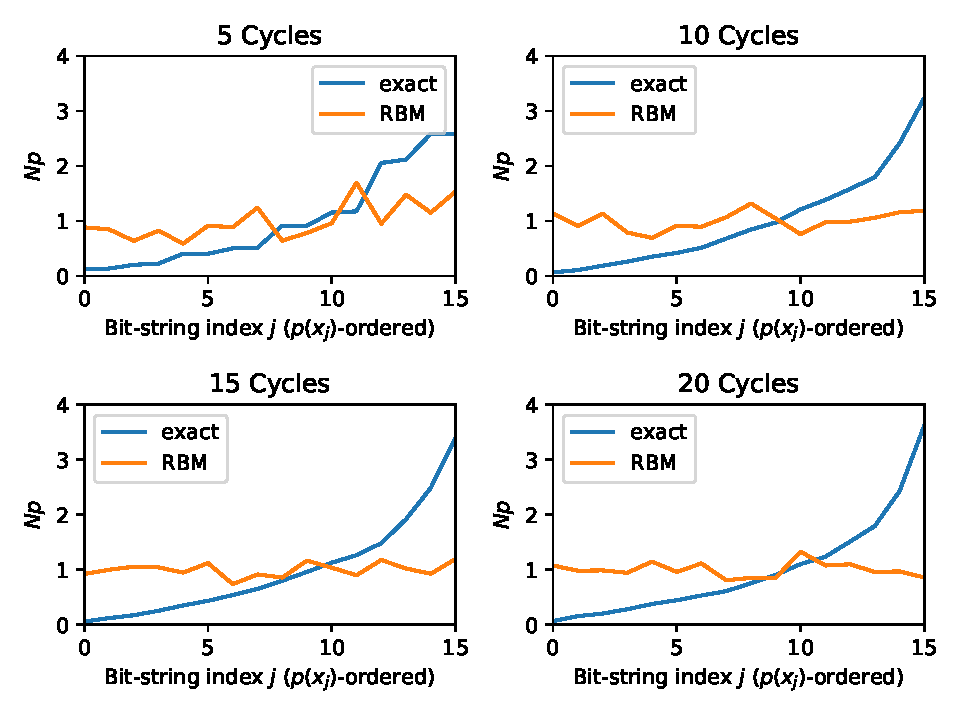
\includegraphics[width=\textwidth]{figures/results/SR-restarts-learned/avgPDF.pdf}
  \caption[Scaled average output probabilities of Stochastic Reconfiguration with Restarts Learned]{
    Scaled average output probabilities of Stochastic Reconfiguration with Restarts and the $CZ$ gates learned. The true 
    output distribution approaches a Porter-Thomas shape with increasing number of cycles.}
  \label{fig:sr_restarts_avgPDF}
\end{figure}

In figure~\ref{fig:sr_restarts_bestPDF}, only the output distribution of the best performing RBMs with respect to the 
TVD are selected and their outputs are averaged. The averaged best output distribution for the SR methods with 
random restarts and $CZ$ gates learned has a TVD of 0.06 for 5, 0.15 for 10, 0.19 for 15, and 0.24 for 20
cycles. The cross entropy difference is 0.65 for 5, 0.47 for 10, 0.39 for 15, and 0.31 for 20 cycles each. 

\begin{figure}[H]
  \centering
  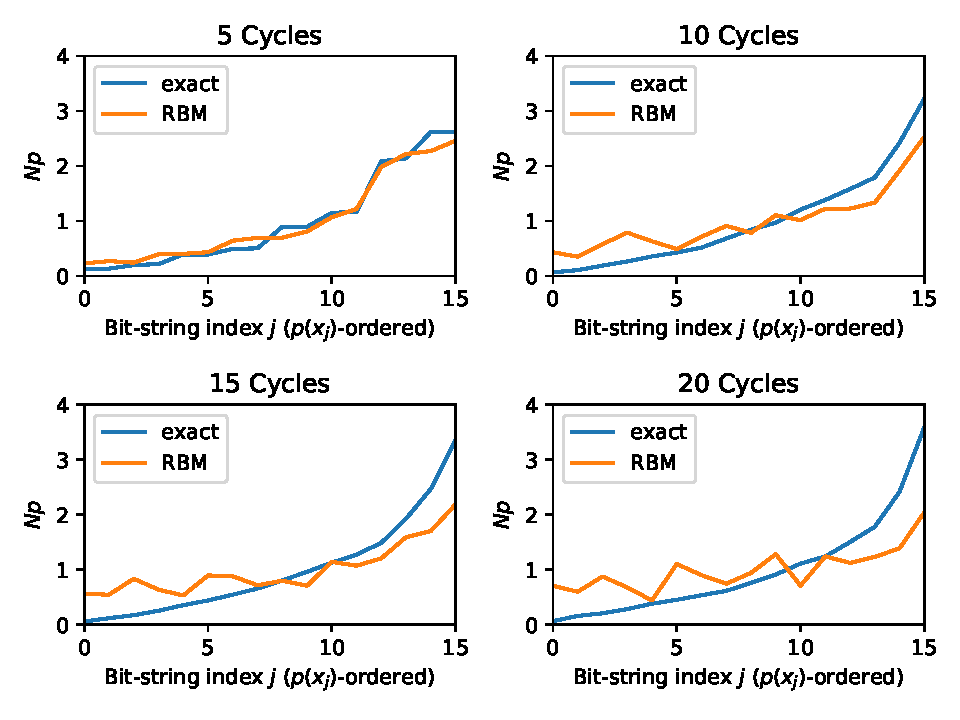
\includegraphics[width=\textwidth]{figures/results/SR-restarts-learned/avgBestPDF.pdf}
  \caption[Averaged best performing scaled output probabilities of Stochastic Reconfiguration with Restarts Learned]{
    Scaled average output probabilities of Stochastic Reconfiguration with Restarts and the $CZ$ gate learned, only RBMs with lowest
    TVD for each circuit are considered.}
  \label{fig:sr_restarts_bestPDF}
\end{figure}

Figure~\ref{fig:sr_restarts_tvd} and figure~\ref{fig:sr_restarts_fxeb} give a more detailed overview of the influence of the 
number of training samples and training iterations on the TVD and cross entropy difference. 

There is no correlation between the number of training
iterations and the performance of the RBMs. For 5 cycles, a higher number of training samples correlates
with a lower TVD, independent of the number of training iterations. The RBMs perform best on 
circuits with a depth of 5 cycles when trained with 100,000 iterations and 303 samples. In that case, 
it achieves a mean TVD of $0.50$. The mean TVD is similar when trained with 303 samples and 1,000 iterations, 
where it is $0.51$. When trained with fewer samples, the TVD is generally lowest when trained with 1,000 
iterations and highest when trained with 10,000 iterations for all number of samples tested. 

For 10 cycles, RBMs trained for 1,000 training iterations achieve the lowest TVDs in the range of 43 to 
54 samples. For 303 samples, 100,000 iterations lead to the lowest TVD (0.59). Except for the 
case of 47 samples, 10,000 iterations correlate with the highest TVD.

For 15 and 20 cycles, again, 10,000 training iterations correlate with the lowest TVD in most cases. 1,000
and 100,000 iterations perform similar, with the lowest TVDs on these circuits being achieved with 50 samples and 
100,000 iterations on 15 cycles ($0.62$), and 47 samples with 100,000 iterations on 20 cycles (TVD of $0.68$).

\begin{figure}[H]
  \centering
  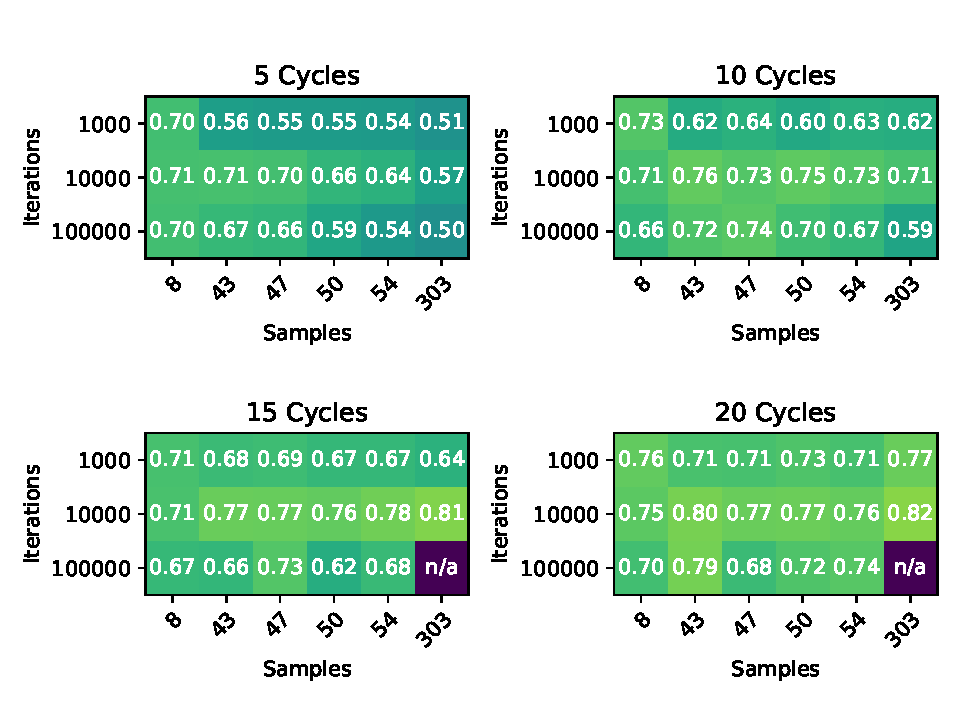
\includegraphics[width=\textwidth]{figures/results/SR-restarts-learned/tvd_heatmap.pdf}
  \caption[TVD of Stochastic Reconfiguration with Restarts Learned]{TVD of Stochastic 
  Reconfiguration with Restarts Learned for the combinations of iterations and samples tested.
  For 100,000 iterations and 303 samples, the experiments did not finish within the time limit.}
  \label{fig:sr_restarts_tvd}
\end{figure}

A lower TVD does not always correlate with a higher cross entropy difference as figure~\ref{fig:sr_restarts_fxeb}
shows. On 5 cycles, the highest fidelity is achieved with 303 samples and 10,000 iterations, on 10 cycles 
with 303 samples and 100,000 iterations. On 15 cycles, 8 samples and 1,000 iterations led to the best performance, 
and 47 samples with 100,000 iterations on 20 cycles. Overall, there is a tendency for a higher cross entropy difference 
when trained with more samples for 5 and 10 cycles. For 15 cycles, there is no clear correlation between the 
cross entropy difference and the training parameters. For circuits with 20 cycles, 47 samples achieved the highest 
fidelity for all number of training samples.

\begin{figure}[H]
  \centering
  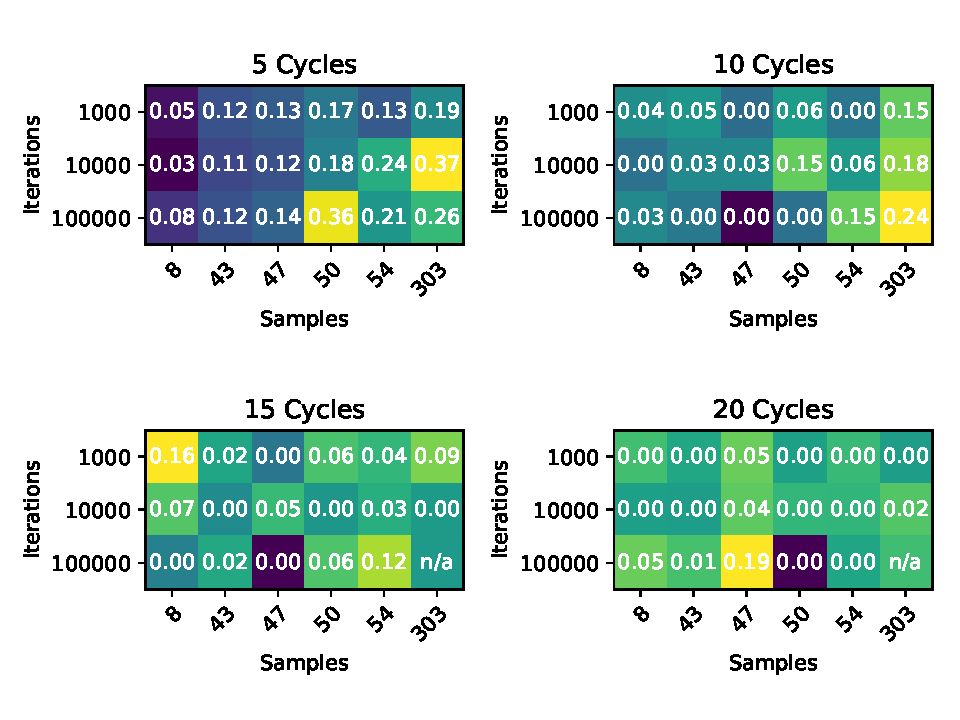
\includegraphics[width=\textwidth]{figures/results/SR-restarts-learned/fxeb_heatmap.pdf}
  \caption[Cross-entropy Fidelity of Stochastic Reconfiguration with Restarts Learned]{Cross-entropy Fidelity of Stochastic 
  Reconfiguration with Restarts and the $CZ$ gates learned for the combinations of iterations and samples tested.}
  \label{fig:sr_restarts_fxeb}
\end{figure}

Figure~\ref{fig:sr_restarts_overlap_8} to~\ref{fig:sr_restarts_overlap_303} details the mean log overlap of the RBMs during the 
training process when trained with 10,000 iterations for 8, 47, and 303 samples. The 
mean overlap of the RBM's state and the distribution implied by the training and test data sets are measured 
for each training iteration.

For 8 samples, the log overlap on the training set can be reduced to almost 0 within the first few training iterations 
on all three gates. For the $\sqrt{Y}$ gate there is a second small dip after about 2,500 training iterations. 
The log overlap on the test set stays slightly below $0.60$ for the single-qubit gates and at about $0.80$ for the 
$CZ$ gate. 

During the whole process and averaged over all three gates, the log overlap is slightly above $0$ in the training data. There is a small 
improvement within the first few training iterations and another small improvement at around 2,500 training iterations. 
The overall log overlap in the test data is about $0.6$ and does not change much during the training process. It 
slightly increases within the first few iterations and goes down a little bit again at about 2,500 training iterations.

\begin{figure}[H]
  \centering
  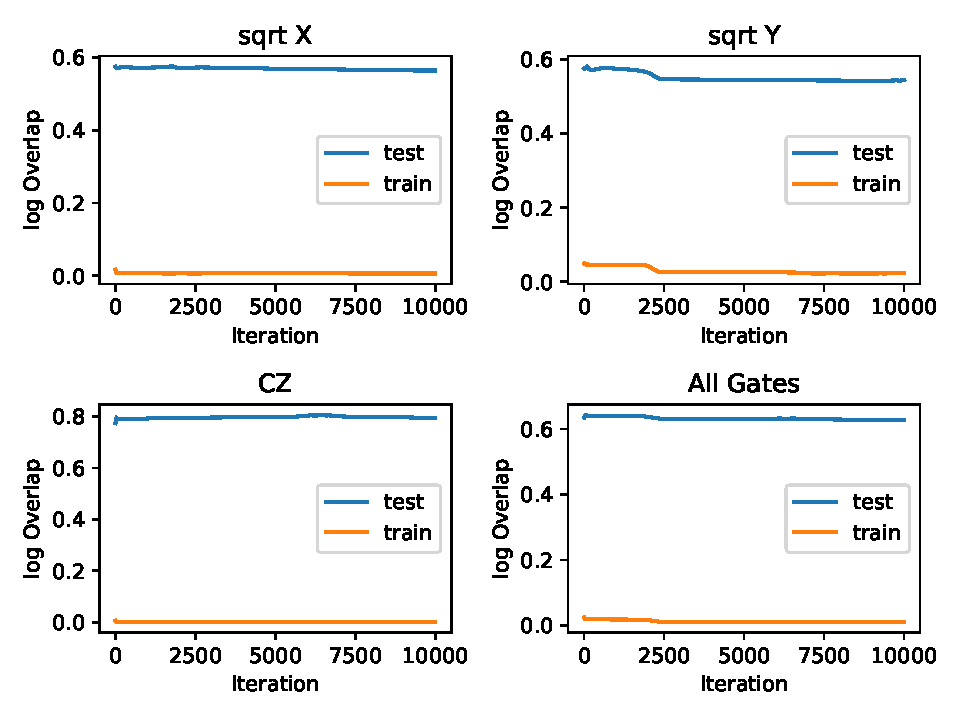
\includegraphics[width=\textwidth]{figures/results/SR-restarts-learned/avgOverlap_8.pdf}
  \caption[Training Overlap of Stochastic Reconfiguration with Restarts Learned]{Training 
  Overlap of Stochastic Reconfiguration with Restarts and the $CZ$ gates learned for 8 samples.}
  \label{fig:sr_restarts_overlap_8}
\end{figure}

For 47 samples, the change in the average training and test overlap is fluctuating during all 10,000
training iterations on all gates. For the 
$\sqrt{X}$ gate, the log overlap on the test set steadily decreases from 
about $0.35$ to about $0.30$. In the same period, the overlap on the training data decreases from about $0.24$ to about $0.21$.

For the $\sqrt{Y}$ gate, the training and test overlaps decrease by about $0.50$ within the first few iterations. 
Afterward, the training overlap slightly increases until about the 2,500th iteration before it decreases again 
until the 10,000th iteration. On the test data, the overlap follows a similar pattern. The 
training overlap is slightly below $0.275$ after 10,000 iterations. The test overlap is at about $0.325$ 
at the end of the 10,000 iterations. 

For the $CZ$ gate, there is an initial drop in the training and testing overlaps. Afterward, 
the training overlap oscillates at around $0.5$ for the first 5.00 iterations before it slowly increases to about 
0.10 after 10,000 iterations. The test overlap oscillates around about 0.16 for the first 5,000 iterations and 
slowly increases to about 0.17 within the following 5,000 iterations. 

Averaged over all gates, the training and test error both drop within the first few iterations to about 
0.20 on the test data and about 0.27 on the training data. Afterward, the overlap slowly decreases to about 0.19 and 
0.24 over the period of 10,000 iterations.

The training and test overlap follows similar pattern for 43, 50, and 54 samples. For 43 samples, the 
overlap is less fluctuating for the $\sqrt{X}$ gate. It reaches lower values on the $\sqrt{Y}$ gate with 
a final testing overlap of about 0.30. The overall overlap on all gates is also lower with about 0.25.

For 50 samples, the final testing overlap is lower for the single qubit gates with about 0.24 on the $\sqrt{X}$
and 0.28 on the $\sqrt{Y}$ gate. The final test overlap is with about 0.15 similar for the $CZ$ gate. On all gates, 
the average final test overlap is about 0.23 with 50 samples.

With 54 samples, the testing overlap on the $\sqrt{X}$ goes down to about 0.23. On the $\sqrt{Y}$ gate it goes 
down to about 0.24, and to about 0.12 on the $CZ$ gate. Over all gate, the testing overlap reaches a value of about 
0.20 after 10,000 iterations when trained with 50 samples.

The graphs for 43, 50, and 54 qubits are included in the appendix.

\begin{figure}[H]
  \centering
  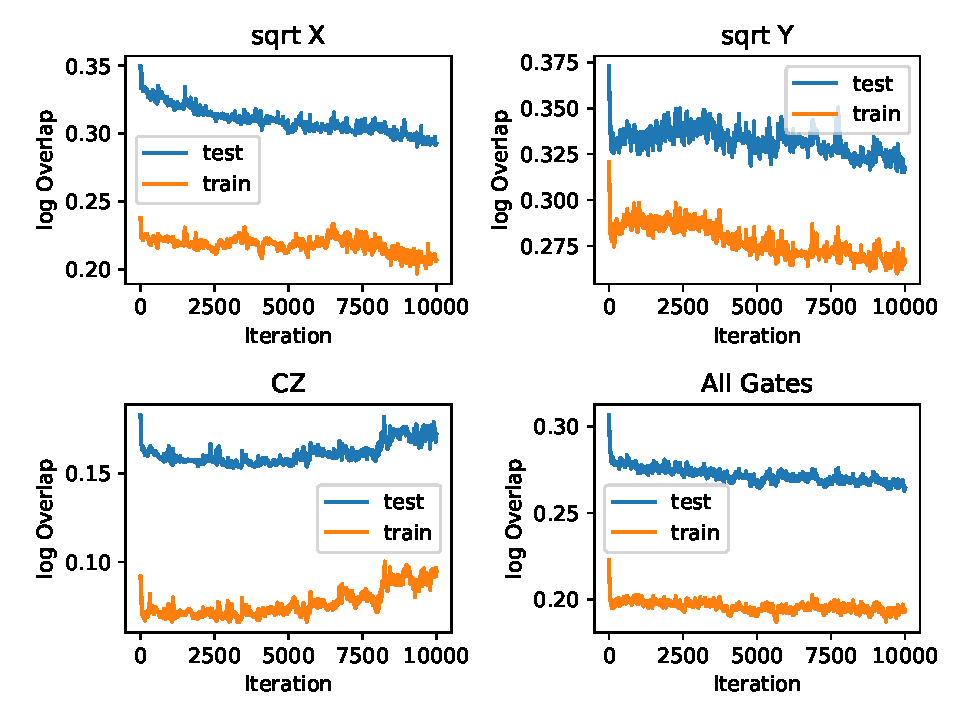
\includegraphics[width=\textwidth]{figures/results/SR-restarts-learned/avgOverlap_47.pdf}
  \caption[Training Overlap of Stochastic Reconfiguration with Restarts Learned]{Training 
  Overlap of Stochastic Reconfiguration with Restarts Learned for 47 samples.}
  \label{fig:sr_restarts_overlap_47}
\end{figure}

With 303 samples, the mean test and training overlaps oscillate even more. The overlap on the training and the 
test data is very close. 

For the $\sqrt{X}$ gate, the overlap drops from about 0.28 to 0.23 within the first very few iterations. 
Afterward, it slowly decreases further to about 0.22 throughout the 10,000 iterations.

On the $\sqrt{Y}$ gate, the overlap has the biggest decrease from about 0.28 to 0.25 within the first 
few iterations. Afterward, it keeps steady to about the 2,500th iteration before it drops to 0.24 at about 5,000 iterations.
Then, it increases again to about 0.255 at about 7,500 iterations and stays in that range for the remaining iterations.

On the $CZ$ gate, the overlap starts at about 0.09 and drops to about 0.06 within the first few iterations. 
For the remaining training process, it slowly increases again to about 0.07. 

Averaged over all gates, the training and testing overlap is about 0.22 at the beginning of the training, 
drops to 0.19 within the first very few iterations and hits a minimum of about 0.18 at about 6,000 iterations before 
it increases again. Starting at about 9,000 iterations, it decreases again to about 0.18.

\begin{figure}[H]
  \centering
  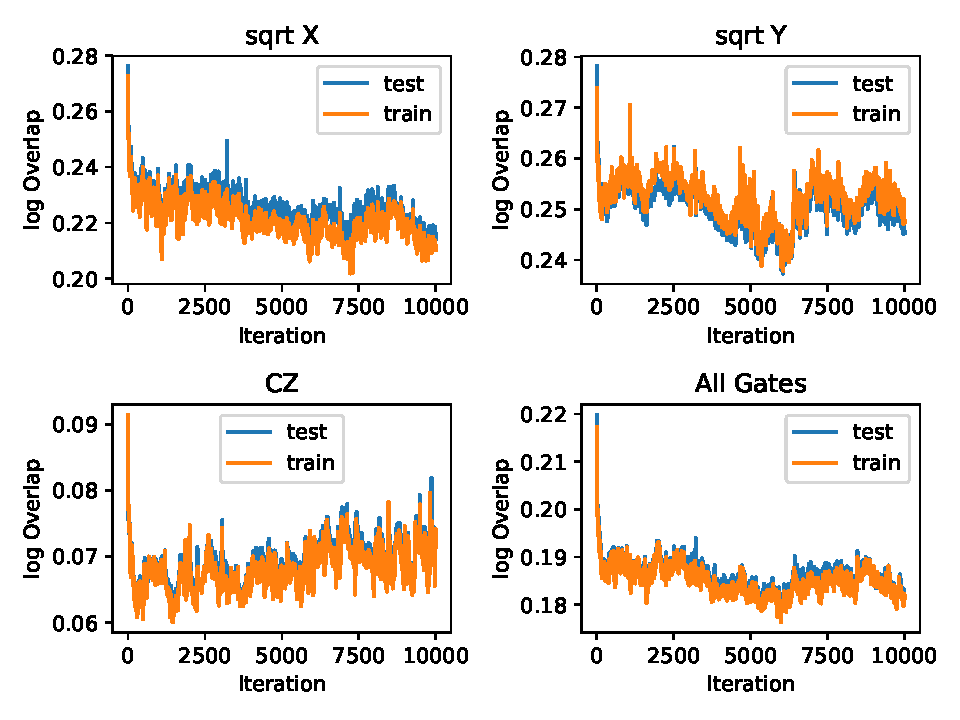
\includegraphics[width=\textwidth]{figures/results/SR-restarts-learned/avgOverlap_303.pdf}
  \caption[Training Overlap of Stochastic Reconfiguration with Restarts Learned]{Training 
  Overlap of Stochastic Reconfiguration with Restarts and the $CZ$ gates learned for 303 samples.}
  \label{fig:sr_restarts_overlap_303}
\end{figure}

\newpage

\subsection{Stochastic Reconfiguration without Random Restarts and CZ Gates Learned}

The last section showed the results for RBMs that were trained with the Stochastic Reconfiguration
method and random restarts. The following section shows the results of RBMs trained without restarts.

Figure~\ref{fig:sr_no_restarts_avgPDF} shows the averaged output distribution of all RBMs and
the averaged true output distributions of all circuits. As before, the 
true output distributions approach a Porter-Thomas shape with an increasing number of cycles.
The TVD of the average output of all RBMs trained with SR without restarts
is 0.34 for 5, 0.38 for 10, 0.34 for 15, and 0.38 for 20 cycles. The corresponding cross entropy is 
0.12 for 5, 0.00 for 10, 0.04 for 15, and 0.00 for 20 cycles.

\begin{figure}[H]
  \centering
  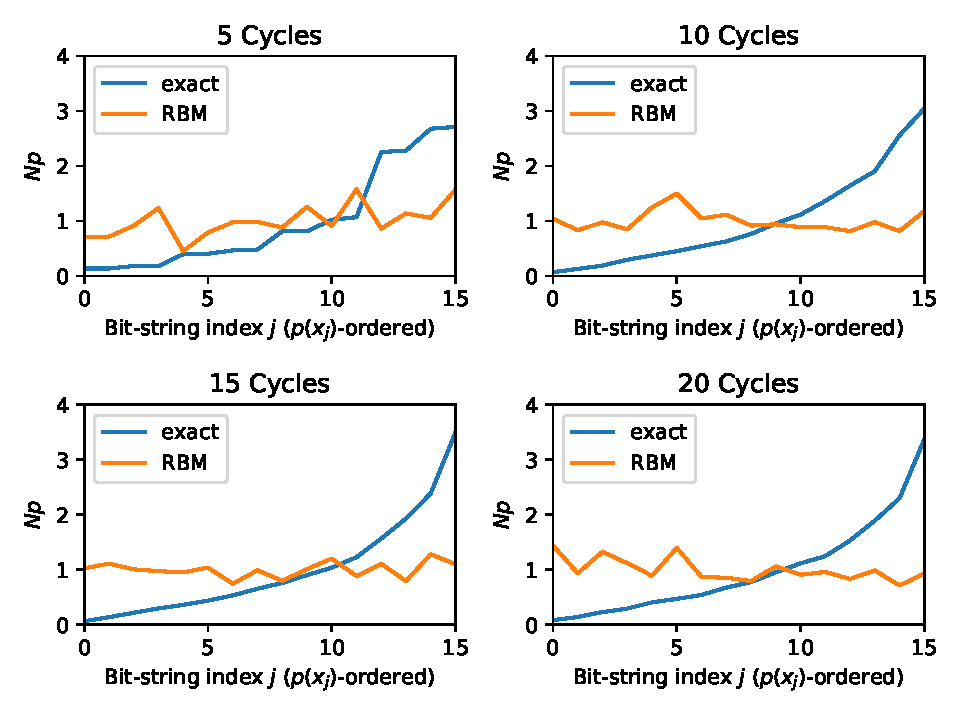
\includegraphics[width=\textwidth]{figures/results/SR-no-restarts-learned/avgPDF.pdf}
  \caption[Scaled average output probabilities of Stochastic Reconfiguration without Restarts Learned]{
    Scaled average output probabilities of Stochastic Reconfiguration without Restarts Learned. The true 
    output distribution approaches a Porter-Thomas shape with increasing number of cycles.}
  \label{fig:sr_no_restarts_avgPDF}
\end{figure}

In figure~\ref{fig:sr_no_restarts_bestPDF}, only the output distribution of the best performing RBMs with respect to the 
TVD are selected and their outputs averaged. The averaged best output distribution for the SR methods without 
random restarts and $CZ$ gates learned has a TVD of 0.07 for 5, 0.18 for 10, 0.21 for 15, and 0.21 for 20 
cycles. The cross entropy difference is 0.71 for 5, 0.37 for 10, 0.40 for 15, and 0.35 for 20 cycles each. 

\begin{figure}[H]
  \centering
  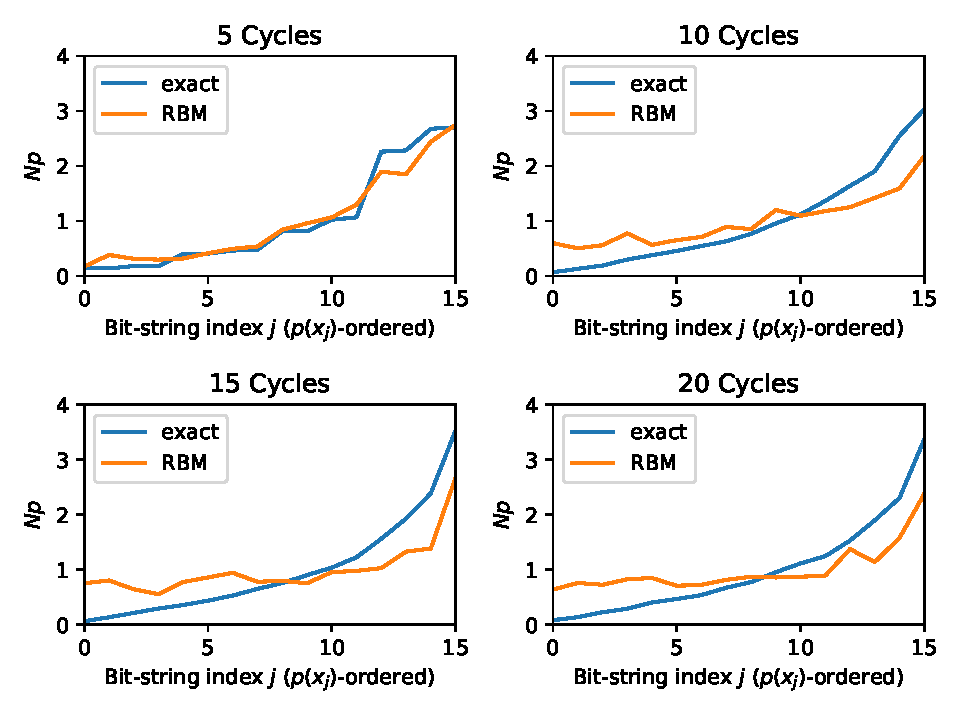
\includegraphics[width=\textwidth]{figures/results/SR-no-restarts-learned/avgBestPDF.pdf}
  \caption[Averaged best performing scaled output probabilities of Stochastic Reconfiguration without Restarts Learned]{
    Scaled average output probabilities of Stochastic Reconfiguration without Restarts Learned, only RBMs with lowest
    TVD for each circuit are considered. The true 
    output distribution approaches a Porter-Thomas shape with increasing number of cycles.}
  \label{fig:sr_no_restarts_bestPDF}
\end{figure}

Figure~\ref{fig:sr_no_restarts_tvd} and figure~\ref{fig:sr_no_restarts_fxeb} give a more detailed overview of the influence of the 
number of training samples and training iterations on the TVD and cross entropy difference achieved by 
the RBMs. Also here, there seems to be no correlation between the number of training
iterations and the performance of the RBMs. 

For 5 cycles, a higher number of training samples 
correlates with an overall lower TVD for 10,000 and 100,000 iterations, but not so for 1,000 iterations. The RBM performs best on 
circuits with a depth of 5 cycles when trained with 100,000 iterations and 303 samples. In this case, 
it achieves a mean TVD of $0.43$. Overall, the performance is independent of the number of 
training iterations when trained with less than 303 samples. In these cases, the performance is very 
similar for 1,000, 10,000, and 100,000 iterations. The only exception is for 54 samples, where 100,000 iterations lead to a 
mean TVD of $0.55$, while the mean TVD is at $0.64$ when trained with 1,000. the mean TVD is $0.62$ when trained for 
10,000 iterations. 

For 10 cycles, 1,000 training iterations achieves the lowest TVDs for 43 or more samples. 
100,000 iterations lead to a lower TVD than 10,000 iterations in all cases. 

For 15 and 20 cycles, again 10,000 training iterations correlate with the highest TVD in most cases.
The performance is similar for all number of training samples. The lowest TVDs are achieved when trained for 1,000
iterations. Also in these cases, the performance is similar for all tested number of training samples; with 
the exception that it is significantly higher for 8 samples.

\begin{figure}[H]
  \centering
  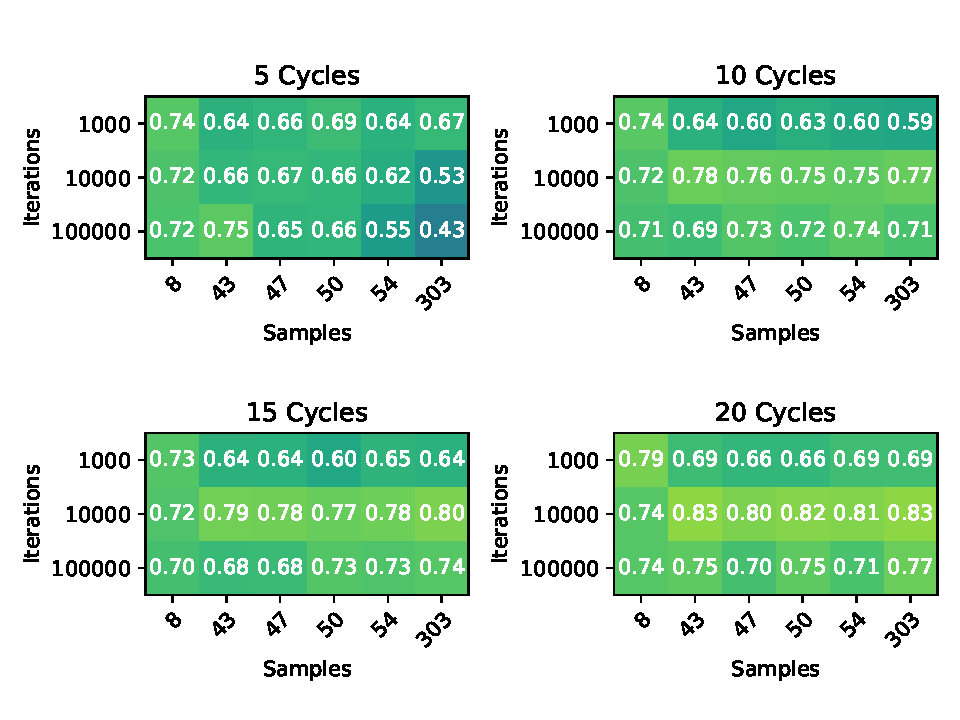
\includegraphics[width=\textwidth]{figures/results/SR-no-restarts-learned/tvd_heatmap.pdf}
  \caption[TVD of Stochastic Reconfiguration without Restarts Learned]{TVD of Stochastic 
  Reconfiguration without Restarts Learned for the combinations of iterations and samples tested.
  For 100,000 iterations and 303 samples, the experiments did not finish within the time limit.}
  \label{fig:sr_no_restarts_tvd}
\end{figure}

As in the case with restarts, a lower TVD does not always correlate with a higher cross entropy difference as 
figure~\ref{fig:sr_no_restarts_fxeb}
implies. For 5 cycles, the highest fidelity is achieved with 303 samples and 10,000 iterations, on 10 cycles 
with 43 samples and 1,000 iterations, with 47 samples and 100,000 iterations on 15 cycles, and with 303 samples and 
0,000 iterations on 20 cycles. There is no clear tendency that shows a correlation between 
the number of training iterations, samples, and cross entropy difference.

\begin{figure}[H]
  \centering
  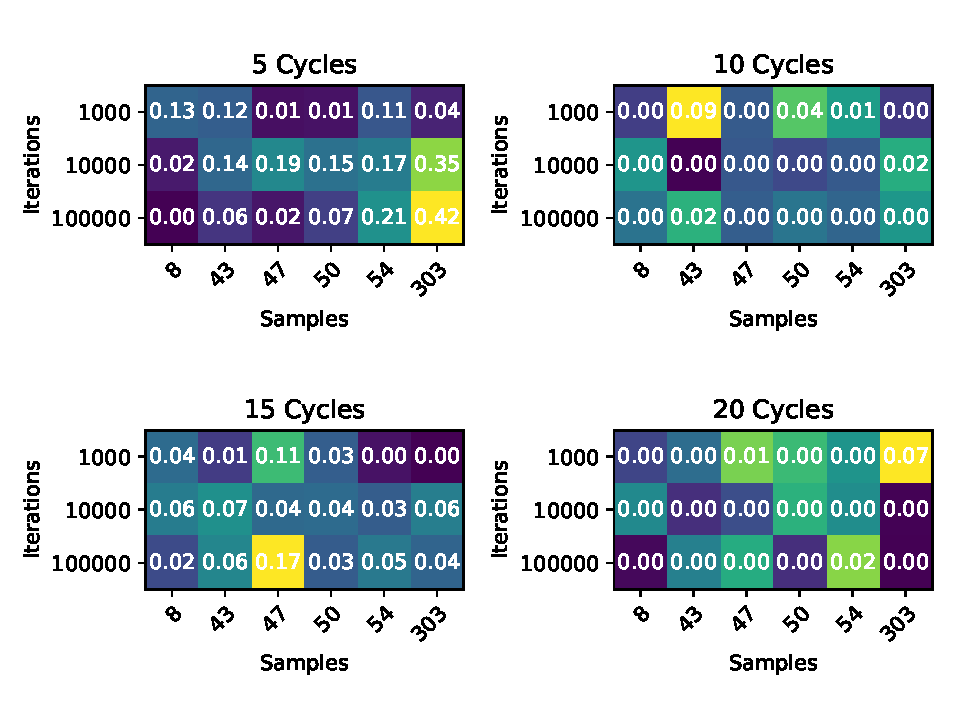
\includegraphics[width=\textwidth]{figures/results/SR-no-restarts-learned/fxeb_heatmap.pdf}
  \caption[Cross-entropy Fidelity of Stochastic Reconfiguration without Restarts Learned]{Cross-entropy Fidelity of Stochastic 
  Reconfiguration without Restarts Learned for the combinations of iterations and samples tested.
  For 100,000 iterations and 303 samples, the experiments did not finish within the time limit.}
  \label{fig:sr_no_restarts_fxeb}
\end{figure}

Figure~\ref{fig:sr_no_restarts_overlap_8} to~\ref{fig:sr_no_restarts_overlap_303} detail the mean log overlap of the RBMs during the 
training process when trained with 10,000 iterations for 8, 47, and 303 samples. The 
mean overlap of the RBM's state and the distribution implied by the training and test data sets are measured 
for each training iteration.

For 8 samples, the log overlap on the training set can be reduced to about 0 for all three gates after about 2,500 iterations.
For the $\sqrt{Y}$ gate, the overlap plateaus at about 0.1 after about 1,000 iterations, before it starts 
to decrease again from 2,000 iterations on. 

The log overlap on the test goes down to about $0.50$ for the $\sqrt{X}$ gate within the first 500 iterations and stays at 
that level for the remaining training process. For the $\sqrt{Y}$ gate, the testing overlap decreases to about 
$0.55$ within the first about 500 iterations. Afterward, it increases again to about 0.60 where it stays for the 
remaining iterations. For the $CZ$ gate, it goes down to about 1.0 within the first 500 iterations and stays at 
that level afterward.

Averaged over all gates, the overlap goes down close to 0 within the first 2,500 training iterations. 
After 500 iterations, the test 
overlap reaches about 0.65 at which it stays for the remaining training iterations. It only 
slightly increases again over the course of the next about 2,000 iterations.


\begin{figure}[H]
  \centering
  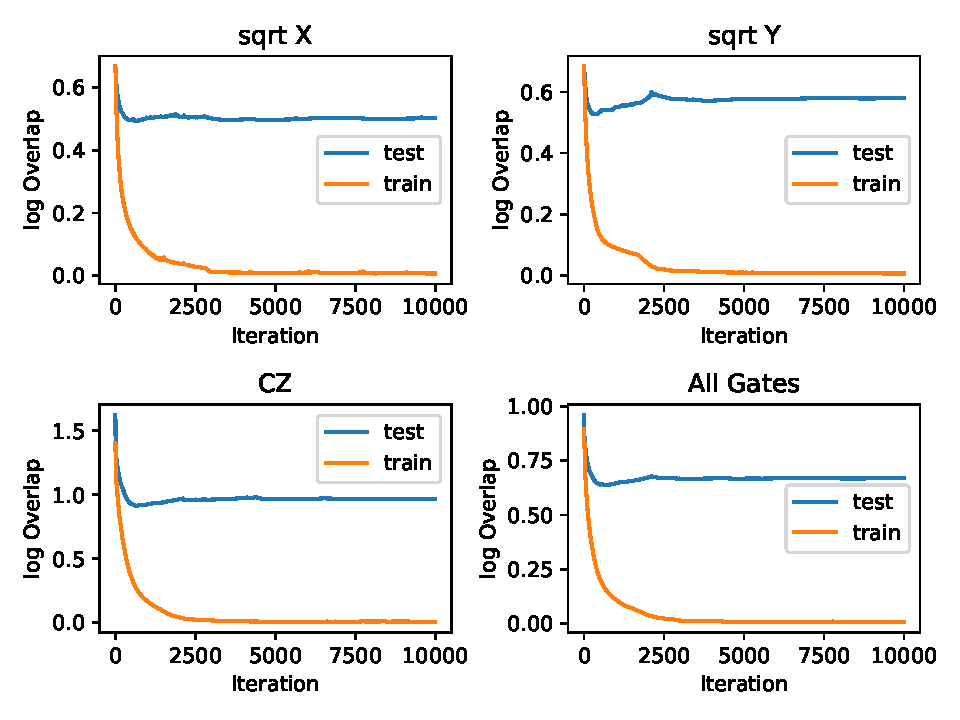
\includegraphics[width=\textwidth]{figures/results/SR-no-restarts-learned/avgOverlap_8.pdf}
  \caption[Training Overlap of Stochastic Reconfiguration without Restarts Learned]{Training 
  Overlap of Stochastic Reconfiguration without Restarts Learned for 8 samples.}
  \label{fig:sr_no_restarts_overlap_8}
\end{figure}

For 47 samples, the change in the average training and test overlap is slightly more fluctuating than for 8 qubits. For the 
$\sqrt{X}$ gate, the log overlap on the training set steadily decreases on the test data set from 
about $0.70$ to about $0.19$ within the first 2,500 training iterations. The overlap on the test data 
decreases to about 0.25 within the same time. Afterward, the training overlap increases again to about 
0.20 within the next 1,500 iterations. At the same time, the overlap on the test data increases to about 
0.3 and stays at that level.

On the $\sqrt{Y}$ gate, the training overlap decreases to about 0.20 within the first 2,500 training iterations 
and stays at that level from thereon. The test overlap decreases to about 0.29 within the first 2,500 iterations 
and also stays there for the remaining part of the training process.

On the $CZ$ gate, the training overlap decreases to about 0.1 in the first 3,000 training iterations. It does 
not change much afterward. The overlap on the test data goes down to about 0.2 within the first 3,500 iterations 
and stays at that level.

Averaged over all gates, the overlap on the test data goes down to about 0.18 within the first 2,500 training iterations. 
The test overlap goes down to about 0.25 in the same time. Both metrics stay at those values afterward.

The training and test overlap follows similar pattern for 43, 50, and 54 samples with the 
test overlap being closer to the training overlap with increasing number of samples. The overall
testing overlap averaged over all gates approaches 0.2 for 54 samples.

The graphs for 43, 50, and 54 qubits are included in the appendix.

\begin{figure}[H]
  \centering
  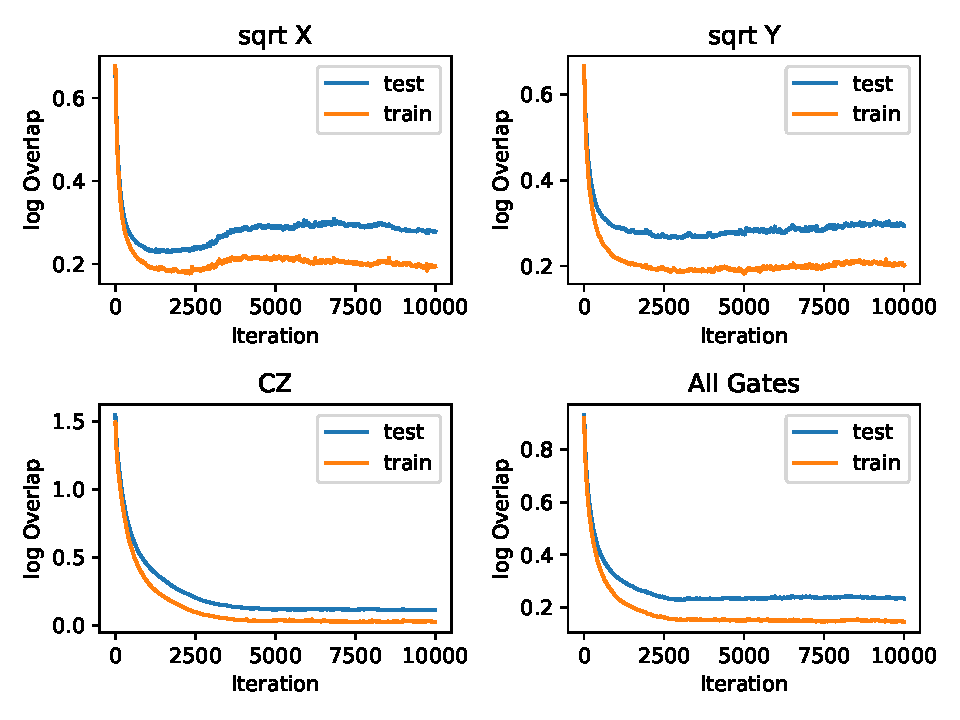
\includegraphics[width=\textwidth]{figures/results/SR-no-restarts-learned/avgOverlap_47.pdf}
  \caption[Training Overlap of Stochastic Reconfiguration without Restarts Learned]{Training 
  Overlap of Stochastic Reconfiguration without Restarts Learned for 47 samples.}
  \label{fig:sr_no_restarts_overlap_47}
\end{figure}

With 303 samples, the curves of the log overlap on the training data look very similar to the 
ones with 47 samples. A noticeable difference can be observed for the test overlap, which is 
about the same as the training overlap in all cases.

\begin{figure}[H]
  \centering
  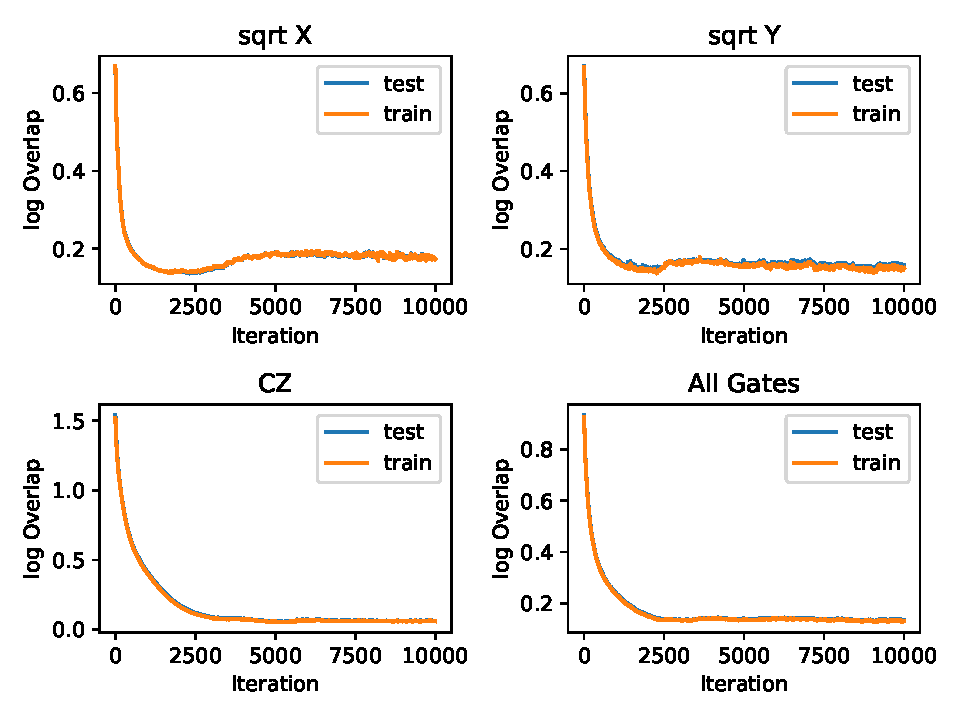
\includegraphics[width=\textwidth]{figures/results/SR-no-restarts-learned/avgOverlap_303.pdf}
  \caption[Training Overlap of Stochastic Reconfiguration without Restarts Learned]{Training 
  Overlap of Stochastic Reconfiguration without Restarts Learned for 303 samples.}
  \label{fig:sr_no_restarts_overlap_303}
\end{figure}

\newpage

\subsection{Stochastic Reconfiguration with Random Restarts and CZ Gates Applied Exactly}

In previous works, the $CZ$ gate had been applied to the RBM state exactly \cite{jnsson2018neuralnetwork}. This study compares 
the performance of RBMs when the $CZ$ gate is applied exactly and learned. The comparison might shed
light on how the training process of a gate is influenced by the number of qubits the gate 
is acting on. It further can give a hint on whether the addition of hidden units by applying the $CZ$
gate exactly influences the training process of the other gates.
The following section shows the results of RBMs trained with restarts and the $CZ$ gates applied 
with the rules from section X.

Figure~\ref{fig:sr_exact_avgPDF} shows the averaged output distribution of all RBMs and
the averaged true output distributions of all circuits. As in the cases before, the 
true output distributions approach a Porter-Thomas shape with an increasing number of cycles.
The TVD of the average output of all RBMs 
is 0.35 for 5, 0.33 for 10, 0.34 for 15, and 0.38 for 20 cycles. The corresponding cross entropy is 
0.20 for 5, 0.02 for 10, 0.06 for 15, and 0.00 for 20 cycles.

\begin{figure}[H]
  \centering
  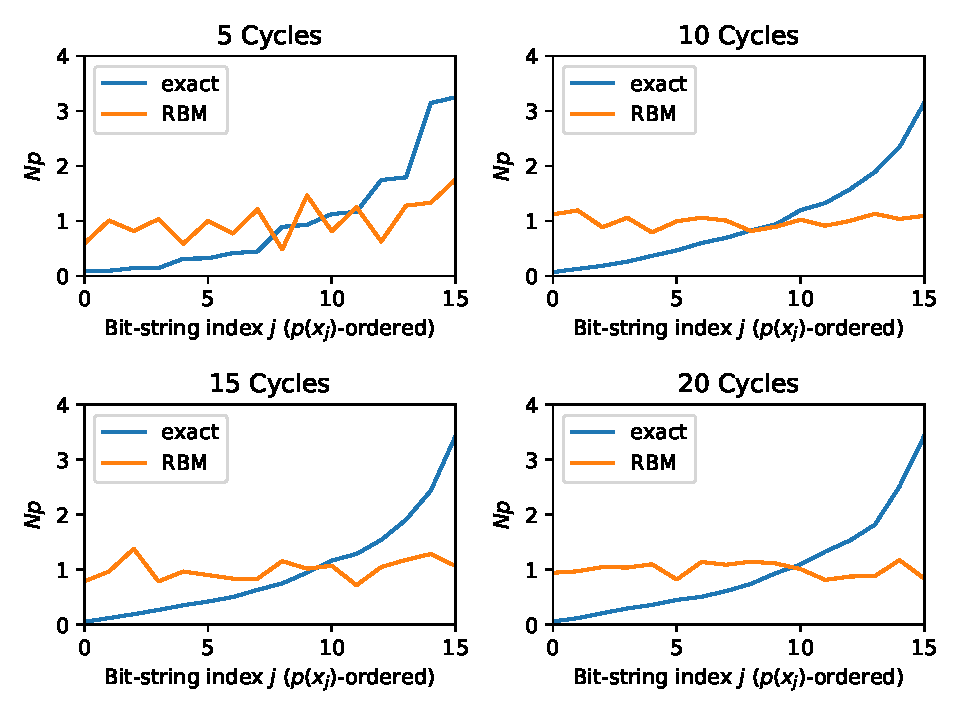
\includegraphics[width=\textwidth]{figures/results/SR-restarts-not-learned/avgPDF.pdf}
  \caption[Scaled average output probabilities of Stochastic Reconfiguration with Restarts Exact]{
    Scaled average output probabilities of Stochastic Reconfiguration with Restarts Exact. The true 
    output distribution approaches a Porter-Thomas shape with increasing number of cycles.}
  \label{fig:sr_exact_avgPDF}
\end{figure}

In figure~\ref{fig:sr_exact_bestPDF}, only the output distribution of the best performing RBMs with respect to the 
TVD are selected. Their outputs are averaged. The averaged best output distribution 
has a TVD of 0.03 for 5, 0.13 for 10, 0.22 for 15, and 0.21 for 20 
cycles. The cross entropy difference is 1.00 for 5, 0.46 for 10, 0.33 for 15, and 0.40 for 20 cycles each. 


\begin{figure}[H]
  \centering
  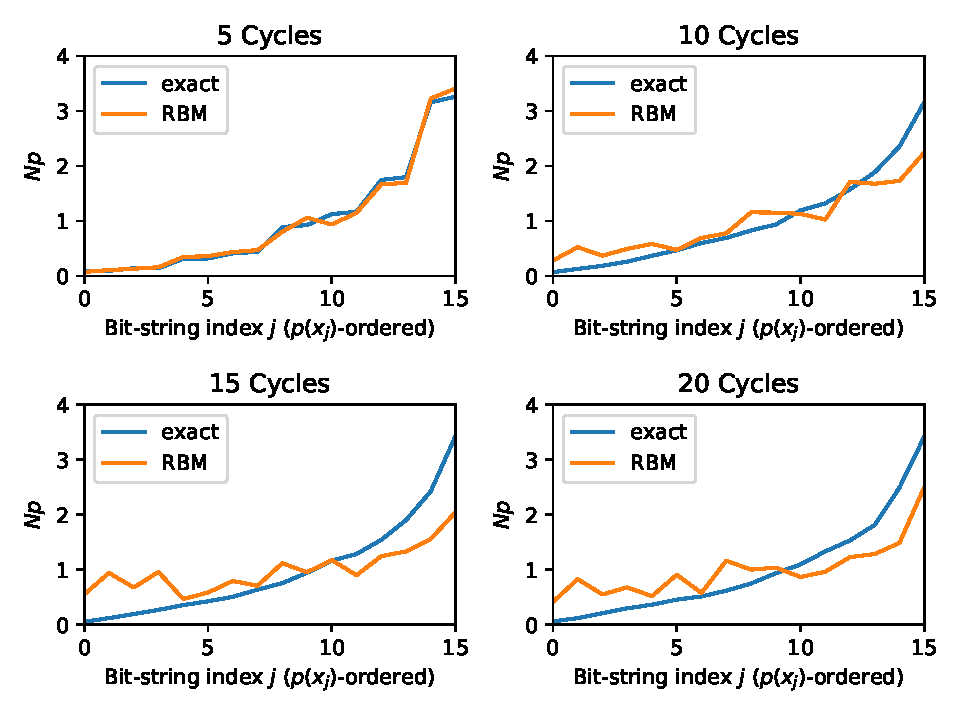
\includegraphics[width=\textwidth]{figures/results/SR-restarts-not-learned/avgBestPDF.pdf}
  \caption[Averaged best performing scaled output probabilities of Stochastic Reconfiguration with Restarts Exact]{
    Scaled average output probabilities of Stochastic Reconfiguration with Restarts Exact, only RBMs with lowest
    TVD for each circuit are considered. The true 
    output distribution approaches a Porter-Thomas shape with increasing number of cycles.}
  \label{fig:sr_exact_bestPDF}
\end{figure}

Figure~\ref{fig:sr_exact_tvd} and figure~\ref{fig:sr_exact_fxeb} detail the influence of the 
number of training samples and training iterations on the TVD and cross entropy difference achieved by 
the RBMs. 

For 5 cycles, a higher number of training samples 
correlates with an overall lower TVD. The RBM performs best on 
circuits with a depth of 5 cycles when trained with 100,000 iterations and 303 samples. In that case, 
it achieves a mean TVD of $0.49$. Overall, the performance is similar for 1,000 and 100,000 iterations.

For 10 cycles, the lowest TVD is also achieved by RBMs trained with 303 samples and 100,000 iterations.
A higher number of samples correlates with an overall lower TVD for 100,000 iterations. For 1,000 iterations, 
the TVD is about 0.60 for 43 samples and higher; and 0.74 for 8 samples. For 10,000 iterations, the TVD varies 
around about 0.75 independent of the number of samples. 

For 15 and 20 cycles, 10,000 training iterations correlate with the highest TVD in most cases.
The performance is similar for all numbers of training samples. The lowest TVDs are achieved with 100,000
iterations and 47 or 54 samples. With 10,000 iterations, a higher number of training samples correlates 
with a higher TVD. For 1,000 and 100,000 iterations, there is no clear difference in the number of training 
samples.

\begin{figure}[H]
  \centering
  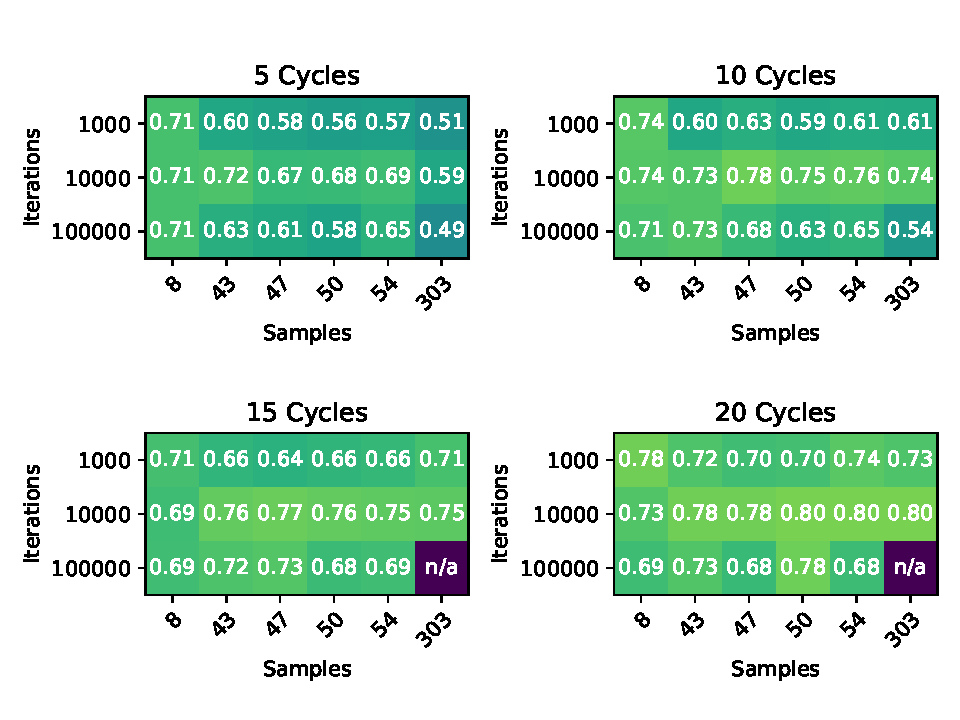
\includegraphics[width=\textwidth]{figures/results/SR-restarts-not-learned/tvd_heatmap.pdf}
  \caption[TVD of Stochastic Reconfiguration with Restarts Exact]{TVD of Stochastic 
  Reconfiguration with Restarts Exact for the combinations of iterations and samples tested.
  For 100,000 iterations and 303 samples, the experiments did not finish within the time limit.}
  \label{fig:sr_exact_tvd}
\end{figure}

Figure~\ref{fig:sr_no_restarts_fxeb} shows the average cross entropy difference achieved. On 5 and 10
cycles, the highest fidelity is achieved with 303 samples and 100,000 iterations. 
For 15 cycles, the highest fidelity is achieved with 50 samples on 100,000 iterations and 
303 samples and 10,000 iterations.
For 20 cycles, the highest fidelity is achieved on RBMs trained with 47 samples for 100,000 iterations.
There is no clear tendency that shows a correlation between 
the number of training iterations or samples and the cross entropy difference.

\begin{figure}[H]
  \centering
  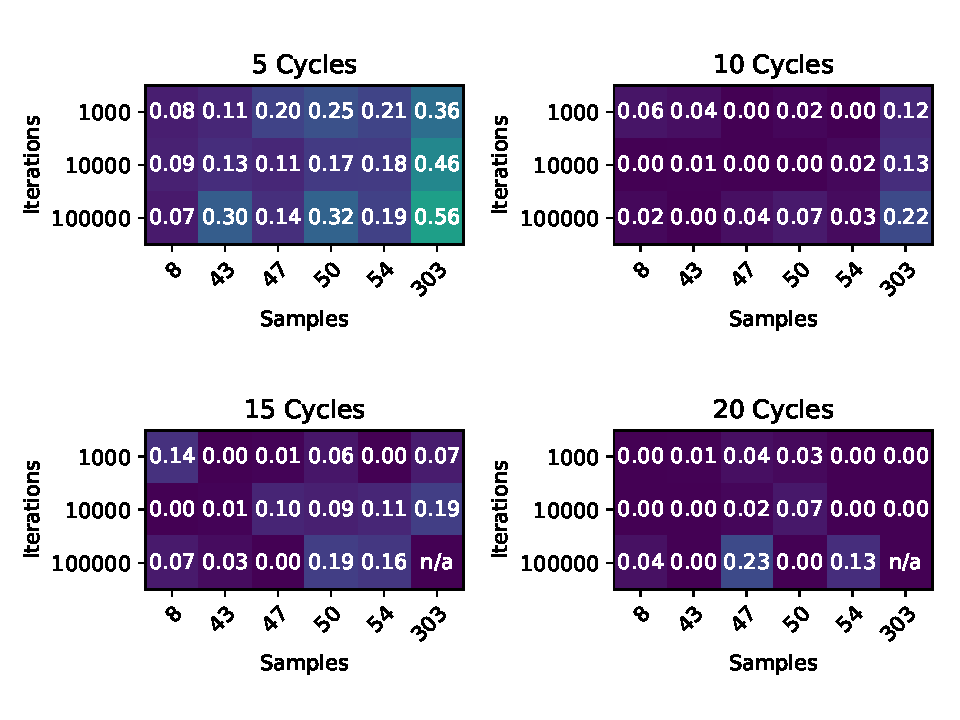
\includegraphics[width=\textwidth]{figures/results/SR-restarts-not-learned/fxeb_heatmap.pdf}
  \caption[Cross-entropy Fidelity of Stochastic Reconfiguration with Restarts Exact]{Cross-entropy Fidelity of Stochastic 
  Reconfiguration with Restarts Exact for the combinations of iterations and samples tested.
  For 100,000 iterations and 303 samples, the experiments did not finish within the time limit.}
  \label{fig:sr_exact_fxeb}
\end{figure}

Figure~\ref{fig:sr_exact_overlap_8} to~\ref{fig:sr_exact_overlap_303} detail the mean log overlap of the RBMs during the 
training process when trained with 10,000 iterations for 8, 47, and 303 samples. The 
mean overlap of the RBM's state and the distribution implied by the training and test data sets are measured 
for each training iteration.

For 8 samples, both the training and the testing overlap don't vary much during the training. The training errors on the $\sqrt{X}$ and 
$\sqrt{Y}$ gate are both close to 0 during the whole training process. The test error is about 0.60.

\begin{figure}[H]
  \centering
  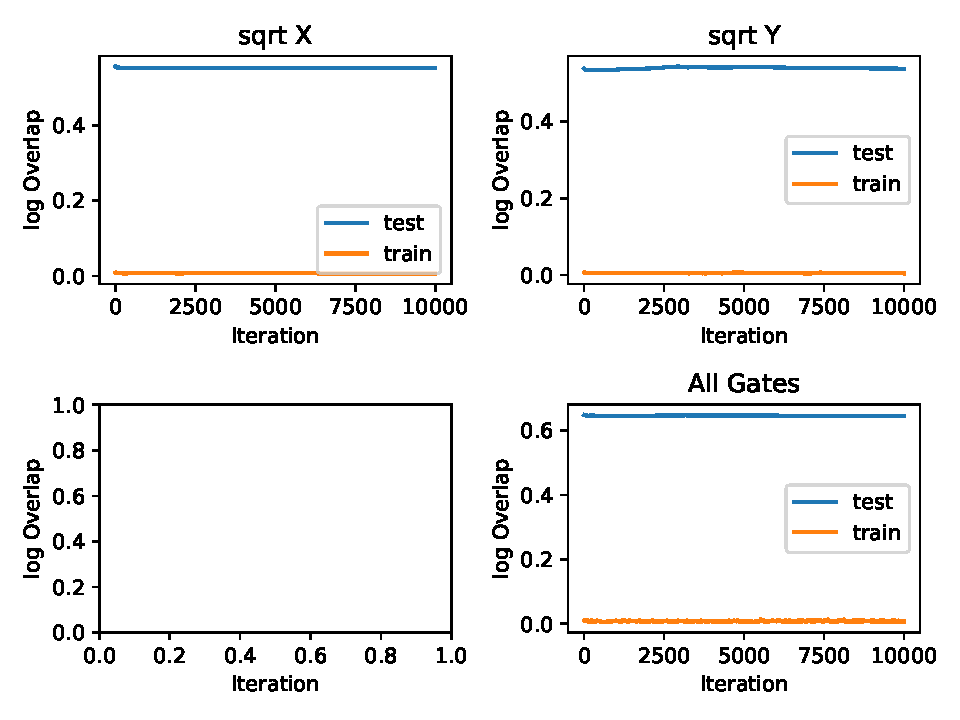
\includegraphics[width=\textwidth]{figures/results/SR-restarts-not-learned/avgOverlap_8.pdf}
  \caption[Training Overlap of Stochastic Reconfiguration with Restarts Exact]{Training 
  Overlap of Stochastic Reconfiguration with Restarts Exact for 8 samples.}
  \label{fig:sr_exact_overlap_8}
\end{figure}

For 47 samples, the change in the average training and test overlap is oscillating. For the 
$\sqrt{X}$ gate, the log overlap on the training set oscillates around about 0.16 during most 
of the training process. It 
reaches its lowest value of about 0.13 after 3,000 iterations. The overlap on the test data 
oscillates around about 0.21 during the whole process. The training error drops from 
0.175 to 0.16 within the first few iterations. The training overlap drops from 0.25 to 0.21 at that time.

On the $\sqrt{Y}$ gate, the training overlap decreases to about 0.17 within the first few training iterations 
and oscillates around that value from thereon. The test overlap decreases to about 0.28 within the first few
iterations and slowly increases to about 0.3 throughout the training process.

The training and test overlap follows similar pattern for 43, 50, and 54 samples.
With 43 samples, the overlaps oscillate less for the $\sqrt{X}$ gate. The testing overlap is about 
0.33 for 43 samples on the $\sqrt{X}$ while the training overlap oscillates around about 0.19.
On the $\sqrt{Y}$ gate, the training overlap is at about 0.16 as for 47 samples. The testing overlap is 
lower and reaches a value of about 0.23 after 10,000 iterations. The averaged testing overlap is higher than 
for 47 samples with a value of about 0.27 and the training overlap is similar with a value of about 0.15.

With 50 and 53 samples, the testing overlap is higher in both cases for the $\sqrt{X}$ gate than for 
47 samples. It is at about 0.29 for 50 samples and about 0.33 for 53 samples. The training overlap is about 
0.21 for 50 samples and about 0.25 for 53 samples on that gate.

On the $\sqrt{Y}$ gate, the testing overlap is with a value of about 0.25 lower in both cases. The 
training overlap on that gate is about 0.18 in both cases. Averaged over both gates, the training 
overlap gets reduced to about 0.18 in both cases while the testing overlap goes down to about 0.25 
throughout the 10,000 iterations.

The graphs for 43, 50, and 54 qubits are included in the appendix.

\begin{figure}[H]
  \centering
  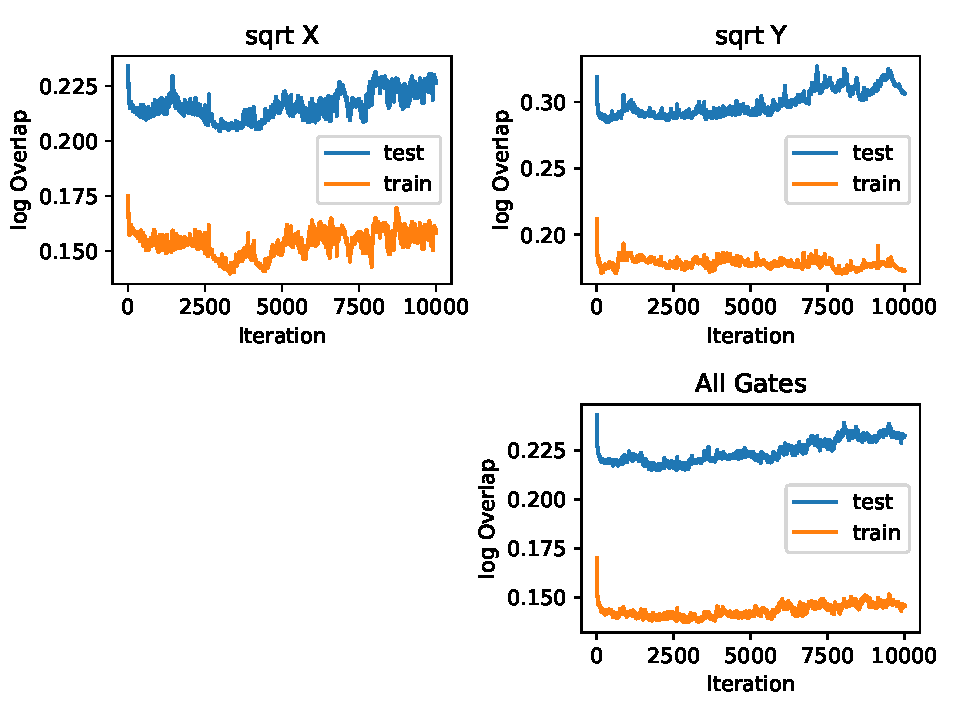
\includegraphics[width=\textwidth]{figures/results/SR-restarts-not-learned/avgOverlap_47.pdf}
  \caption[Training Overlap of Stochastic Reconfiguration with Restarts Exact]{Training 
  Overlap of Stochastic Reconfiguration with Restarts Exact for 47 samples.}
  \label{fig:sr_exact_overlap_47}
\end{figure}

With 303 samples, the oscillation in the test and training overlap is even more than for 47 samples. 
For the $\sqrt{X}$ gate, both values drop to about 0.21 within the first 1,000 training iterations. 
Afterward, the overlaps increase to about 0.25 at 6,000 iterations. It decrease to about 0.24 in the 
remaining part of the training process again.

The process looks similar for the $\sqrt{Y}$ gate. The overlap goes down to about 0.22 within the 
first 1,000 iterations. Afterward, it goes up to about 0.24 again and stays at that level for the 
following training iterations.

\begin{figure}[H]
  \centering
  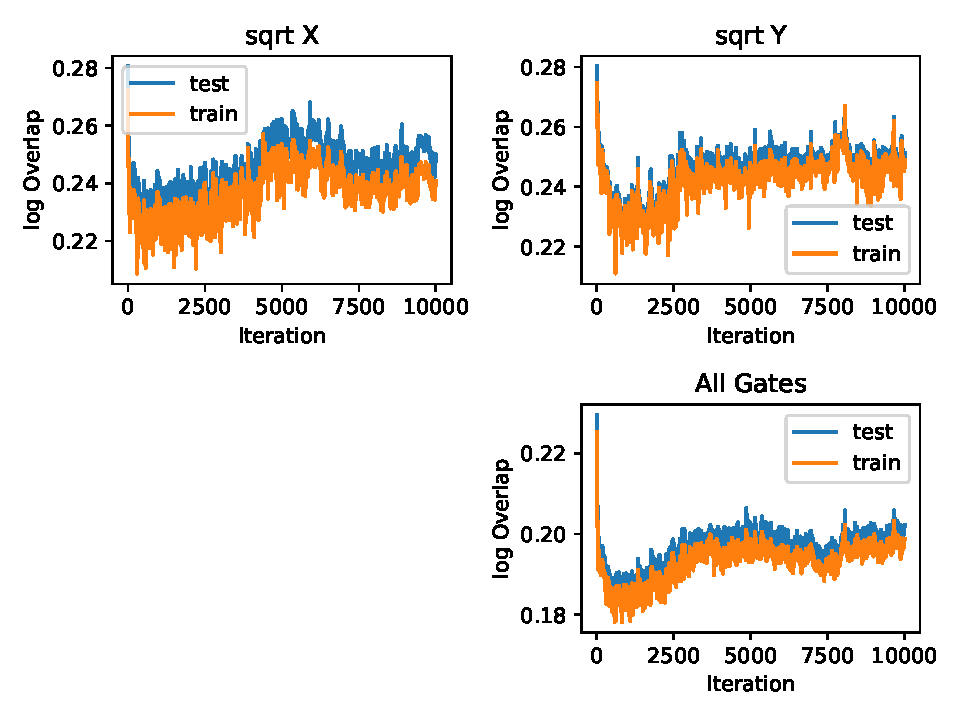
\includegraphics[width=\textwidth]{figures/results/SR-restarts-not-learned/avgOverlap_303.pdf}
  \caption[Training Overlap of Stochastic Reconfiguration with Restarts Exact]{Training 
  Overlap of Stochastic Reconfiguration with Restarts Exact for 303 samples.}
  \label{fig:sr_exact_overlap_303}
\end{figure}

\newpage

\subsection{AdaMax with Random Restarts and CZ Gates Learned}

AdaMax had also been used for training RBMs for the 
classical simulation of quantum circuits before \cite{jnsson2018neuralnetwork}. The following section presents the results
of RBMs trained with AdaMax and five random restarts. The $CZ$ gates are also applied with the 
learning approach in these cases.

Figure~\ref{fig:am_avgPDF} shows the averaged output distribution of all RBMs trained with AdaMax and 
the averaged true output distributions of all circuits. As in the other cases, the 
true output distributions approach a Porter-Thomas shape with an increasing number of cycles.
The TVD of the average output of all RBMs trained with AdaMax
is 0.25 for 5, 0.30 for 10, 0.35 for 15, and 0.33 for 20 cycles. The corresponding cross entropy is 
0.20 for 5, 0.08 for 10, 0.06 for 15, and 0.04 for 20 cycles.

\begin{figure}[H]
  \centering
  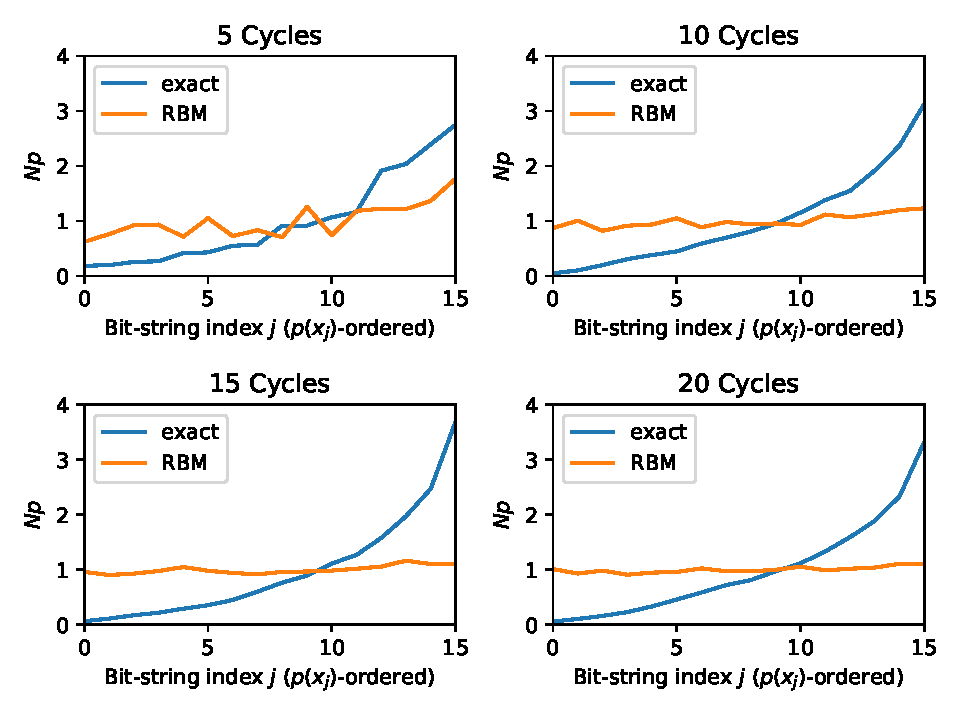
\includegraphics[width=\textwidth]{figures/results/AM-restarts-learned/avgPDF.pdf}
  \caption[Scaled average output probabilities of AdaMax with Restarts Learned]{
    Scaled average output probabilities of AdaMax with Restarts Learned. The true 
    output distribution approaches a Porter-Thomas shape with increasing number of cycles.}
  \label{fig:am_avgPDF}
\end{figure}

In figure~\ref{fig:am_avgBestPDF}, only the output distribution of the best performing RBMs with respect to the 
TVD are selected. Their outputs are averaged once again. The averaged best output distribution 
has a TVD of 0.00 for 5, 0.00 for 10, 0.00 for 15, and 0.00 for 20 
cycles. The cross entropy difference is 0.65 for 5, 0.72 for 10, 0.94 for 15 and 0.77 for 20 cycles each. 

\begin{figure}[H]
  \centering
  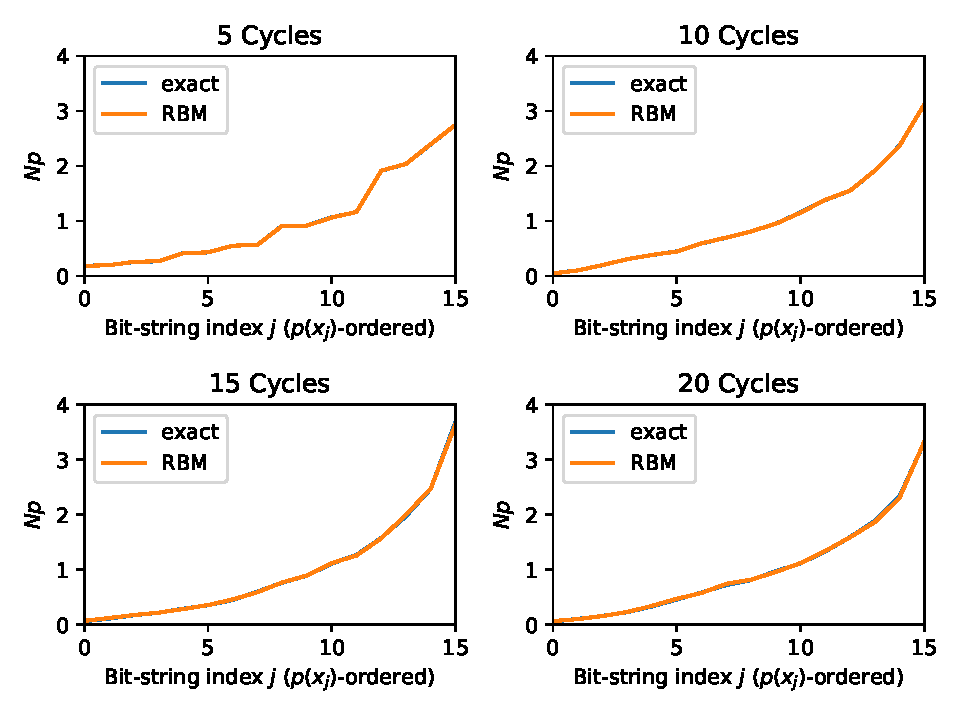
\includegraphics[width=\textwidth]{figures/results/AM-restarts-learned/avgBestPDF.pdf}
  \caption[Averaged best performing scaled output probabilities of AdaMax with Restarts Learned]{
    Scaled average output probabilities of AdaMax with Restarts Learned, only RBMs with lowest
    TVD for each circuit are considered. The true 
    output distribution approaches a Porter-Thomas shape with increasing number of cycles.}
  \label{fig:am_avgBestPDF}
\end{figure}

Figure~\ref{fig:am_tvd} and figure~\ref{fig:am_fxeb} give a more detailed overview of the influence of the 
number of training samples and training iterations on the TVD and cross entropy difference.

Except for the case of 8 samples, for AdaMax a higher number of training samples as well as a higher 
number of training iterations corresponds to a lower TVD. For 5 and 10 cycles, the TVD is lowest
when trained with 303 samples and 100,000 iterations. In these cases, it approaches 0.

For 15 and 20 cycles, the training process could not finish
within the given time frame with this combination of training parameters. On these circuits, the lowest TVDs have been achieved with 303 samples 
and 10,000 iterations.

Overall, the difference between 10,000 iterations and 100,0000 iterations is smaller than between 
1,000 iterations and 10,000 iterations. For 43 to 54 samples, the performance is similar in all cases.
Nevertheless, the TVD is lower with 54 samples than with 43 samples in all but one cases.

\begin{figure}[H]
  \centering
  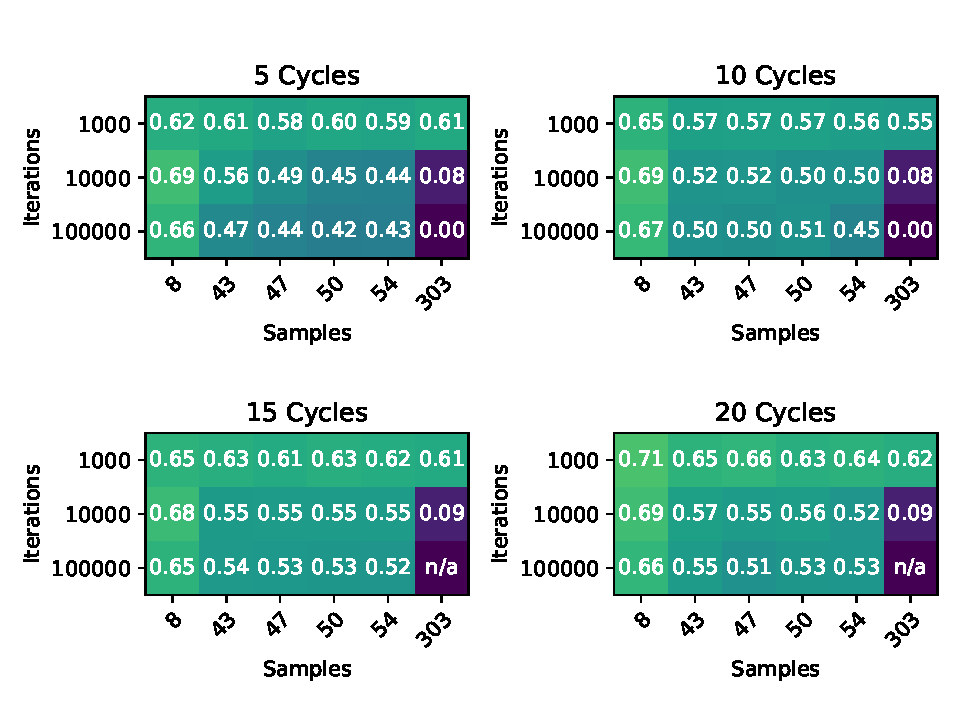
\includegraphics[width=\textwidth]{figures/results/AM-restarts-learned/tvd_heatmap.pdf}
  \caption[TVD of AdaMax with Restarts Learned]{TVD of Stochastic 
  Reconfiguration with Restarts Learned for the combinations of iterations and samples tested.
  For 100,000 iterations and 303 samples, the experiments did not finish within the time limit.}
  \label{fig:am_tvd}
\end{figure}

Figure~\ref{fig:am_fxeb} shows the average cross entropy difference achieved. In contrast to the case 
of TVD, a higher number of training samples and training iterations does not correlate with higher 
fidelities. Only in the case of 5 cycles, this correlation can be observed for 10,000 and 100,000 iterations.

The highest fidelities for 5 and 10 cycles are achieved for 303 samples and 100,000 iterations. For 
15 and 20 cycles, they are achieved with 303 samples and 10,000 iterations. 

In the case of 15 cycles, the overall highest fidelity of 0.90 had been measured. The highest fidelity is 0.65 for 5, 0.75 for 10, and 0.73 for 20 cycles.
This once again demonstrates that a lower TVD does not translate to a higher fidelity directly.

\begin{figure}[H]
  \centering
  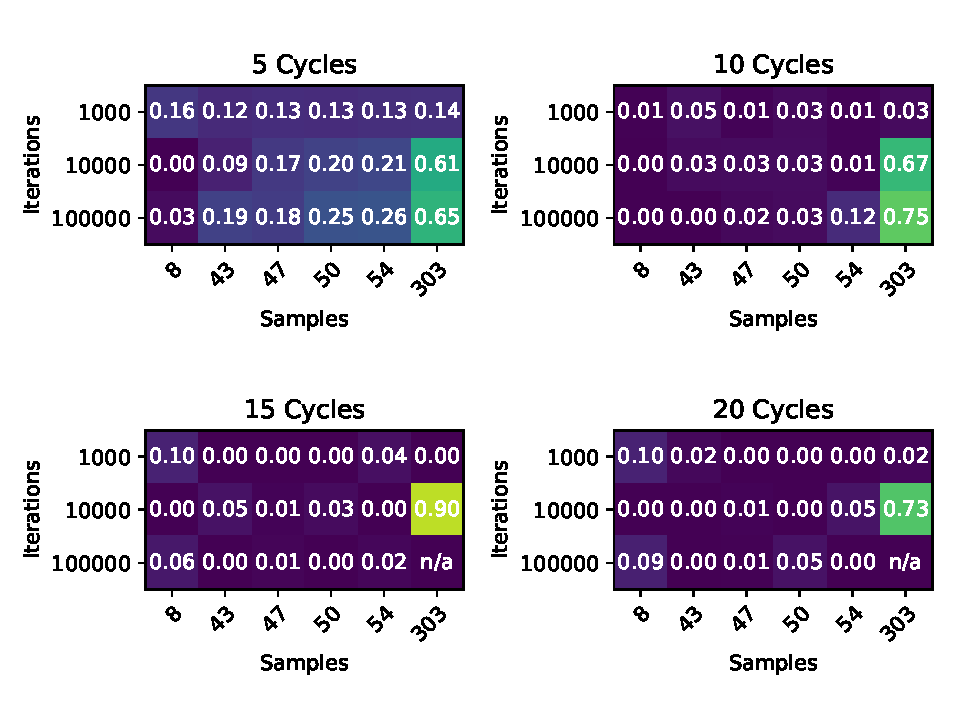
\includegraphics[width=\textwidth]{figures/results/AM-restarts-learned/fxeb_heatmap.pdf}
  \caption[Cross-entropy Fidelity of AdaMax with Restarts Learned]{Cross-entropy Fidelity of Stochastic 
  Reconfiguration with Restarts Learned for the combinations of iterations and samples tested.
  For 100,000 iterations and 303 samples, the experiments did not finish within the time limit.}
  \label{fig:am_fxeb}
\end{figure}

Figure~\ref{fig:am_overlap_8} to~\ref{fig:am_overlap_303} detail the mean log overlap of the RBMs during the 
training process when trained with 10,000 iterations for 8, 47, and 303 samples. The 
mean overlap of the RBM's state and the distribution implied by the training and test data sets are measured 
for each training iteration.
For 8 samples, the training and test overlaps don't vary much during the training process. The training errors on all three gates
close to 0 during the whole training process. The test error is at about 0.40 on the single-qubit gates. It is about 
0.9 on the $CZ$ gate.

\begin{figure}[H]
  \centering
  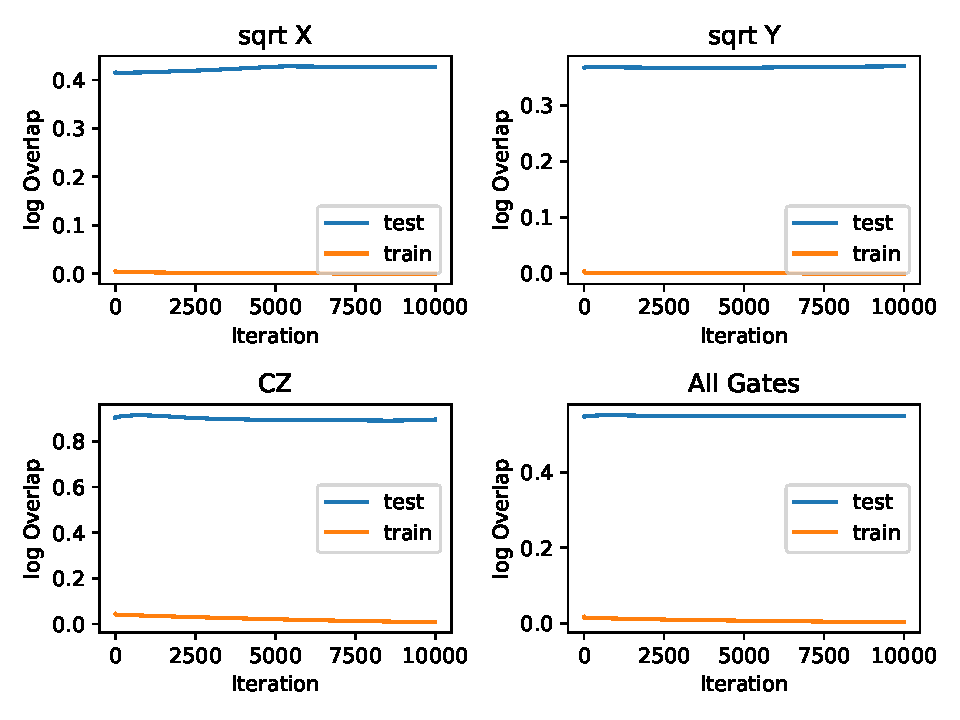
\includegraphics[width=\textwidth]{figures/results/AM-restarts-learned/avgOverlap_8.pdf}
  \caption[Training Overlap of AdaMax with Restarts Learned]{Training 
  Overlap of AdaMax with Restarts Learned for 8 samples.}
  \label{fig:am_overlap_8}
\end{figure}

For 47 samples, the log overlap on the training data drops almost to 0 within the first few iterations 
of training. There is only a small improvement to be observed in the $\sqrt{Y}$ gate afterward. 
The overlap on the test data drops to about 0.1 in the case of $\sqrt{X}$ gates within the first few iterations.
Afterward, there is a slight tendency upwards but the overlap stays in about that range. In the case 
of $\sqrt{Y}$ gates, the test overlap drops to about 0.11 within the first few iterations. Afterward, 
it slightly increases again before it reaches 0.11 after about 2,500 iterations again.

The log overlap looks different for the $CZ$ gate: After an initial drop of about 0.02 to 0.12, the 
training overlap slowly decreases until it reaches a value close to 0 . The 
training overlap takes a similar course. During the training process, it goes down to about 0.18, after 
starting at about 0.33.

The training and test overlap follow a similar course for 43, 50, and 54 samples. For 43 samples, the 
testing overlap reaches values slightly above 0.15 for the $\sqrt{X}$ and $\sqrt{Y}$ gate. On the $CZ$ gates, 
the overlap is only very slightly higher.

For 50 and 54 samples, the testing error goes down to about 0.075 for the $\sqrt{X}$ and $\sqrt{Y}$ gates. 
On the $CZ$ gates, the testing overlap goes down to about 0.15 over the course of the training. The graphs 
for 43, 50, and 54 qubits are included in the appendix.

\begin{figure}[H]
  \centering
  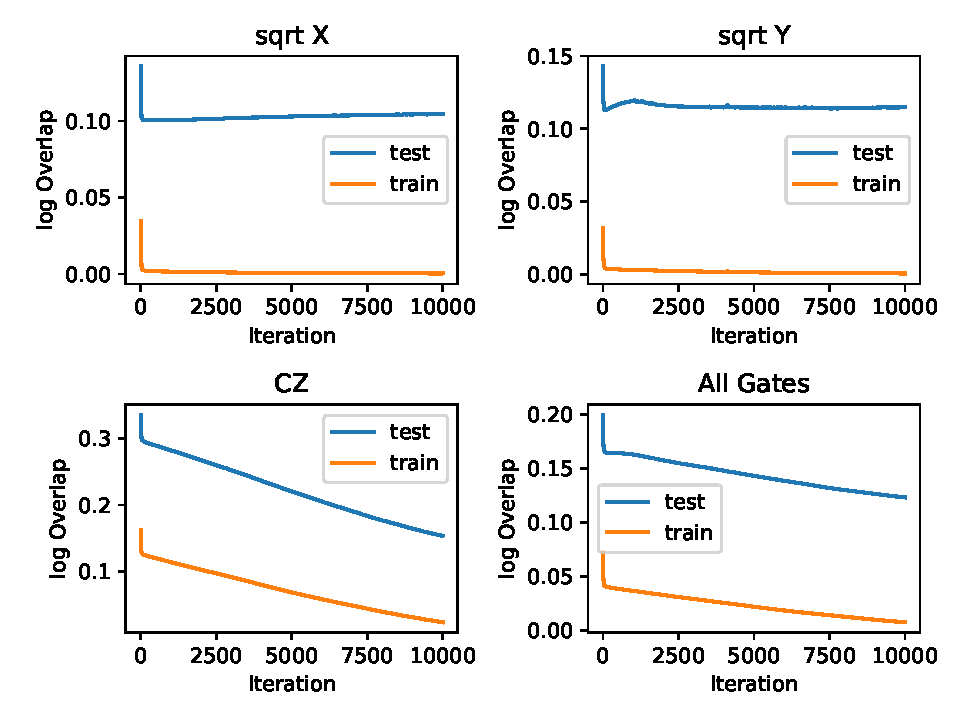
\includegraphics[width=\textwidth]{figures/results/AM-restarts-learned/avgOverlap_47.pdf}
  \caption[Training Overlap of AdaMax with Restarts Learned]{Training 
  Overlap of AdaMax with Restarts Learned for 47 samples.}
  \label{fig:am_overlap_47}
\end{figure}

For 303 training samples, the course of the training overlap is very similar to 47 samples.
A difference can be observed in the test overlap, which is very close to the training overlap 
throughout the whole training process.

\begin{figure}[H]
  \centering
  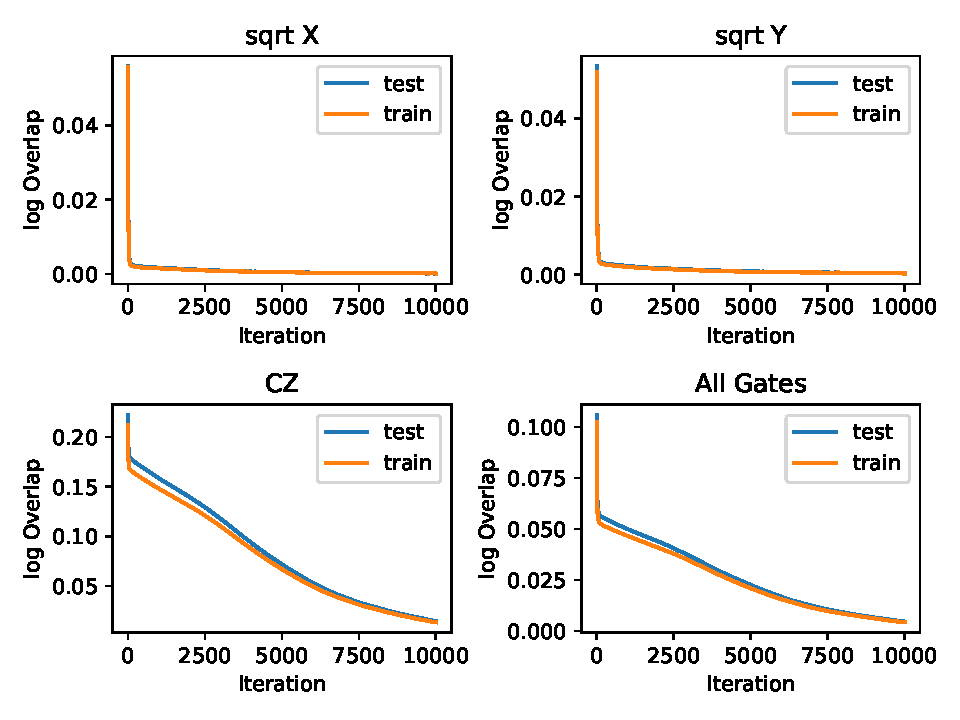
\includegraphics[width=\textwidth]{figures/results/AM-restarts-learned/avgOverlap_303.pdf}
  \caption[Training Overlap of AdaMax with Restarts Learned]{Training 
  Overlap of AdaMax with Restarts Learned for 303 samples.}
  \label{fig:am_overlap_303}
\end{figure}

\chapter{Conclusion and Discussion}
\label{sec:discussion}

\paragraph{Highlights.}
The results of the experiments show that \gls{rbm}s are able to accurately simulate random circuit 
instances with 4 qubits and a depth of up to 20 cycles. The comparison of 
Stochastic Reconfiguration (\gls{sr}) and AdaMax as optimization algorithms suggests that 
AdaMax is better suited for the given gate set and circuit structure with the chosen training 
parameters. The best performing \gls{rbm}s were able to approximate the average true output 
distribution with a \gls{tvd} of 0.00 on all circuit depths. Less than 100 training iterations were sufficient to 
apply non-diagonal single-qubit gates to the state represented by the \gls{rbm}s. 
The more training samples were available, the better the \gls{rbm}s resembled the target output distributions.

\paragraph{Performance of Stochastic Reconfiguration.}
The high \gls{tvd}s of \gls{rbm}s trained with the \gls{sr} methods might be grounded in the algorithm finding 
local minima. These might be optimal only for a subset of the state space. The oscillation for \gls{sr} could be explained by the algorithm finding an 
optimum for one training batch, which does not generalize well to the other training samples.
This would also explain why there is no oscillations for \gls{sr} with restarts on 8 samples. In that
cases, all training samples are inside the same batch. Increasing the batch size or reducing the 
number of hidden units could improve the performance of the \gls{sr} algorithm.

\paragraph{Effects of Random Restarts.}
Using \gls{sr} with random restarts had only small if any 
impact on the resulting accuracy of the \gls{rbm}s. However, the testing and training overlaps 
look different during the training process. Without the restarts, there is not much 
oscillation in these metrics. This supports the assumption that with restarts, the 
\gls{rbm} is overfitting the current training batch, which does not generalize well to training 
samples in other batches. 

This does not imply that this would also 
hold for AdaMax. Indeed, pre-studies suggested that random restarts might have a positive 
impact on the \gls{rbm}'s accuracy when trained with AdaMax.

\paragraph{Effects of Learning the $CZ$ Gate.}
There was no significant difference in the \gls{tvd}s between \gls{rbm}s to which the $CZ$ gates have 
been applied directly and those that learned the $CZ$ gates. At least for the given circuit 
sizes, this implies that adding more hidden units to the \gls{rbm} during the simulation of 
quantum circuits had no significant effect on the training of the single-qubit non-diagonal 
gates. 

These results suggest that for the given gate set and circuit structure, the $CZ$ gates can 
be applied directly to the \gls{rbm}'s state. This significantly reduces the number of gates which 
have to be applied through a learning phase on the given kind of random circuits.

\paragraph{Performance of AdaMax.}
The training and testing overlaps for AdaMax show that the single-qubit gates can 
be learned within less than 100 training iterations. Applying 
the $CZ$ gates directly will omit the need for more training iterations for the given \gls{rbm} size.

Further, it seems that the more training samples are available, the better the \gls{rbm} will 
perform when trained with AdaMax. More experiments will be necessary 
to understand how the number of samples scales with the number of qubits. Establishing
a relation between the number of training samples and the resulting gate fidelity would 
be a major step in understanding the capabilities of \gls{rbm}s for the classical simulation of 
quantum circuits.

\paragraph{Influence of the Number of Training Samples.}
In the conducted experiments, 303 samples were enough to sample each configuration of the 
$2^n$ dimensional state space multiple times. Only for 8  samples, the full state space
could not be observed during the training. The performance of the \gls{rbm}s trained with 8 samples
had been very low. Only if \gls{rbm}s can achieve acceptable performance with a number of samples 
that does not scale exponentially with the number of qubits, this approach would be useful for 
real-world applications. 

In this regard, this study lacks on interpretable insights. Rather than making use of the 
Coupon-collectors problem, it would have been possible to train the \gls{rbm}s with less samples. 
The training and test sets could have been made up of a defined number of different 
samples. This might have given clearer insights into the relation between the ratio of the 
state space observed and the resulting \gls{rbm} performance. For future research, the samples should
be drawn that way.

\paragraph{\gls{rbm}s for the Classical Simulation of \gls{nisq} algorithms.}
Noisy simulations with 
fidelities in the range of that from the Sycamore processor could help to understand the 
capabilities and limits of \gls{nisq} devices using \gls{rbm}s on classical computing hardware. 
For 10 qubits, for instance, the cross entropy difference
of the Sycamore processor was estimated to be around 0.4. On the 4 qubit circuits with 
15 cycles, the fidelity of the best performing \gls{rbm} is at about 0.9. 
If \gls{rbm}s are able to simulate quantum circuits with a similar accuracy as the Sycamore 
processor on a larger number of qubits with acceptable computational requirements, this 
would make \gls{rbm}s a suitable simulation framework to test \gls{nisq} algorithms.

\paragraph{Cross Entropy Difference as a Performance Metric.}
The cross entropy difference was specifically designed to measure the 
ability of an algorithm or device to sample from the output distributions of 
random circuits. In the conducted experiments, it was also possible to 
calculate the \gls{tvd} between the \gls{rbm}'s output and the true output distributions of 
the random circuit instances. The results show that a low \gls{tvd} did not guarantee a 
high cross entropy distance. The reasons for this could be twofold: First, the 
cross entropy distance assumes a depolarizing noise model of the quantum computation. 
Such a model might not be applicable to \gls{rbm}s. Second, the considered circuits have been 
close to Porter-Thomas, but did not generate perfect Porter-Thomas output distributions.
These two reasons might explain that the cross entropy distance and \gls{tvd} did not 
always correlate in the conducted experiments. Nevertheless, the cross entropy distance 
was highest for \gls{rbm}s trained with AdaMax, which also reached the lowest \gls{tvd}s.

\paragraph{Future Research.}
Understanding the ability of \gls{rbm}s to simulate random circuits with a wider range of qubits 
was already intended for this work. However, the performed experiments 
on 4 qubit random circuits took already 8 weeks. Testing \gls{rbm}s with the same 
level of detail on a range of up to 20 qubits was estimated to take up to 
a year. This would have exceeded the time limits of a Master's thesis. Maintenance work on the Noctua Cluster 
after the first batch of experiments made it impossible to conduct more experiments.

Nevertheless, the software developed in the progress of this work is available open source. 
This makes it easy to adapt the code to conduct experiments 
with other ranges of parameters and quantum circuits. For the given kind of random circuit 
sampling experiments, everything is set up to perform more experiments on a broader range of 
qubits. Such experiments could further investigate the empirical relation of \gls{tvd} and cross entropy 
distance. Additionally, they could help to establish a relation between the number of samples and 
the accuracy of the \gls{rbm}s' simulations.

The framework can also be easily used to simulate other \gls{nisq} algorithms. This could help to 
understand such algorithms when no physical device is available and how the algorithm
behaves with different levels of noise in the computation.

This thesis is the first to apply \gls{rbm}s to the simulation of random circuit instances. 
The developed software is publicly available on GitHub \cite{NQS2020} and can be used to simulate arbitrary quantum 
circuits provided in the QASM format. The results from 
this thesis give a reference for suitable training parameters which have not been included in related works.




%%
\bibliography{biblio}

\appendix
\chapter{Additional Experimental Outcomes}
Additional visualisation of the experimental outcomes can be found on the GitHub repository of this thesis at \url{https://github.com/stubbi/masterthesis/tree/master/appendix}.

\end{document}
